%-----------------------------------------------------
% Chapter 2: Características
%-----------------------------------------------------
\chapter{Marco teórico}
\label{chap: cap2}
\section{Desarrollo Colaborativo de Productos (CPD)}

La complejidad creciente de los productos, así como la personalización de los mismos a las particularidades de cada cliente, hace necesario la participación de especialistas para acortar los ciclos de desarrollo de producto y de puesta en el mercado. Tradicionalmente se consideraba la figura de contratistas, a los que se entregaban los planos para que construyeran las distintas partes que integran un proyecto de cualquier sistema. Los contactos se producían de forma presencial y obligaban a frecuentes viajes para mantener el proyecto bajo control.\cite{Ruiz} \vskip
El concepto teórico de CPD como lo conocemos hoy en día tuvo su primer aparición en 1994, en un artículo de Peter Cassidy \footnote{\url{https://books.google.com.ar/books?id=bw0AAAAAMBAJ&lpg=PP1&pg=PA58#v=onepage&q&f=false}} en la revista CIO titulado "Multimedia Comes of Age". Sin embargo, la colaboración en el desarrollo de productos tiene antecedentes anteriores en el libro "The sources of innovation" de Eric Von Hippel \cite{VonHippel1988} en 1988. 
En 1995 apareció en más publicaciones como Complexities of Collaborative Product Development de Margaret Bruce, Fiona Leverick y Dale Littler \cite{Complex1995}. En esa época el enfoque se hacía sobre la relación entre compradores y proveedores, la complejidad misma del desarrollo colaborativo de productos y sus factores de éxito. Posteriormente, la temática fue apareciendo con más frecuencia en artículos periodísticos y presentaciones de papers en todo el mundo. \textcolor{red}{Obviamente} esto no excluye la posibilidad de existencia de conceptos anteriores similares o equivalentes. 


\subsection{Definiciones sobre el CPD}
En 1995, Bruce, Leverick y Littler \cite{Complex1995} describieron la visión de CPD como un medio efectivo para reducir el tiempo de desarrollo y el riesgo organizacional. Además declararon que el desarrollo colaborativo de productos es una proceso evolutivo y cómo la forma, el alcance de su iniciación y la continuación pueden cambiar en el tiempo.

El CPD está definido por la Asociación de gestión de desarrollo de productos en inglés \textit{Product Development Management Association} (PDMA) \footnote{http://www.pdma.org/} desde 1996 como: \textquote{... cuando dos o más empresas deciden colaborar en el desarrollo de productos como socios mutuos, y esto difiere del concepto de externalización por el nivel de asociatividad, ya que las empresas colaboradoras están vinculadas en el proceso de entregar la solución final al cliente o al usuario}. \vskip

Si bien con esta definición se puede comprender al CPD como colaboración entre agentes externos, hay otras como la de R. Del Rosario en el 2003 que lo describe como \textquote{la aplicación de prácticas de colaboración en equipo a los esfuerzos de desarrollo de productos dentro de una organización y además abarca la concurrencia, la atención al ciclo de vida, los proveedores y la tecnología de información en un entorno centrado en el cliente}\cite{Mesbah2007}.

Con respecto a la toma de desiciones, Marija Jankovic describe las implicaciones del contexto industrial colaborativo moderno durante el proceso de desarrollo del producto: \textquote{En este proceso, cada actor tiene objetivos definidos para su dominio de acción. Por lo tanto, la toma de decisiones en colaboración es un proceso donde los actores tienen objetivos diferentes y a menudo contradictorios. Los actores en el proceso colaborativo de toma de decisiones tienen también diferentes grados de conocimientos sobre el problema, así como diferentes informaciones y puntos de vista}\cite{Marija2006}.

En este trabajo el concepto de CPD no se usa específicamente para la colaboración externa o interna de una empresa, sino que incluye elementos de colaboración y toma de decisiones entre personas independientemente de la organización a la que pertenece, por ejemplo: la colaboración para diseñar un producto entre un diseñador industrial y una persona sin formación específica como puede ser un emprendedor.\vskip

En este contexto, el diseño tiene una importancia fundamental, ya que incorpora la información que define todos los pasos, hasta la elaboración final del producto. Puede decirse que la máxima eficacia se logra mediante la adecuación de esta etapa y es lo que realmente influye en el resultado final del producto.\vskip 

\textcolor{red}{
Para una efectiva colaboración no basta con una comunicación iterativa en la que se intercambian pocos datos del producto y siempre de arriba hacia abajo (“top-down”), sino que es necesario disponer de un repositorio común de datos\footnote{Un repositorio, depósito o archivo es un sitio centralizado donde se almacena y mantiene información digital, habitualmente bases de datos o archivos informáticos.} que vayan más allá de la geometría representada en planos, incluyendo documentos de especificaciones, instrucciones de
montaje, etc. y todos ellos en cualquier formato digital: texto, CAD/CAM/CAE, PDM, audio, vídeo y combinaciones de ellos.
Saber trabajar en colaboración se convierte en un valor agregado, sobre todo si ésta es suministradora de componentes o sistemas para ser integrados en el producto final y para lograr esto es indispensable aprovechar el contexto actual de las nuevas tecnologías web y sus posibilidades. \cite{Ruiz} }

\subsection{Diseño}
\textquote{ISO 9000:2000, la Norma que contiene el vocabulario de la Familia ISO 9000, define DISEÑO (Y DESARROLLO) como:
Conjunto de procesos que transforma los requisitos en características especificadas, o en la especificación de un producto, proceso, o sistema.Perdiendo un poco de rigor, Diseñar es crear o definir cómo debe ser algo que satisface nuestros requisitos. Se trata de idear algo que no existe, o que no sabemos que existe. Sabemos qué función debe cumplir “ese algo”, pero no cómo debe ser, necesitamos diseñarlo.}\cite{Pereiro2005}



\subsection{Co-diseño}

La irrupción del diseño colaborativo como paradigma está cambiando el panorama de la práctica del diseño porque está permitiendo la aparición de nuevos dominios de creatividad colectiva. 

El co-diseño o diseño colaborativo se refiere a cómo se aplica la creatividad colectiva a través de toda la duración de un proceso de diseño. El concepto ha surgido tanto como un efecto de la globalización como también gracias a que se considera una potencial herramienta con la cual enfocar el desarrollo de productos, en una industria que requiere
nuevas tecnologías y procesos para abordar el diseño de artefactos cada vez más complejos y satisfacer de esta manera las altas expectativas de los clientes. 
El co-diseño es definido por el hecho de que la creatividad de los diseñadores se une a la de personas que tienen otros perfiles y trabajan juntas en el proceso de elaboración del diseño.
En esta definición se plantean los dos elementos fundamentales que soportan el paradigma de diseño colaborativo:

\textbf{a) Nuevos perfiles}\vskip
En esta nueva forma de ver el diseño, al grupo habitual de trabajo se suman la iniciativa y la creatividad de otros perfiles que hasta ahora aportaban ideas generalmente como agentes externos: el investigador, el cliente y la persona que finalmente se beneficiará con el
resultado del co-diseño: el usuario.
En el diseño colaborativo estos perfiles tienden a mezclarse: El usuario pasa a jugar un rol de “experto en su experiencia” y puede aportar elementos de valor en la generación de conceptos e ideas en una etapa inicial de desarrollo. La labor del investigador, a partir de la experiencia del usuario, será proporcionar herramientas acertadas para recoger todos los datos que dicho perfil puede aportar y, a la vez, puede desempeñar un papel fundamental en dar forma a las ideas. De ahí la idea de que el investigador y el diseñador puede ser la misma persona.

\textbf{b) Objetivo en común}\vskip
La idea del objetivo compartido se plantea como una de las principales diferencias con respecto a los métodos tradicionales del diseño de productos o artefactos. Los métodos de diseño generalmente se planteaban para ser llevados a cabo por expertos que
realizaban tareas individuales. Con el trabajo individual no era necesario compartir la visión del objetivo general del proceso de diseño. En cambio, el diseño colaborativo plantea que este punto es fundamental: Para que el equipo funcione correctamente necesita tener la visión del objetivo en común.

Lógicamente, después de apuntar las características principales del diseño colaborativo, se infiere que el rol del diseñador en el proceso debe cambiar necesariamente al incluir este nuevos ''socios'' creativos en un entorno que tradicionalmente le pertenecía. \cite{Huerta2013}

\begin{figure}
\centering
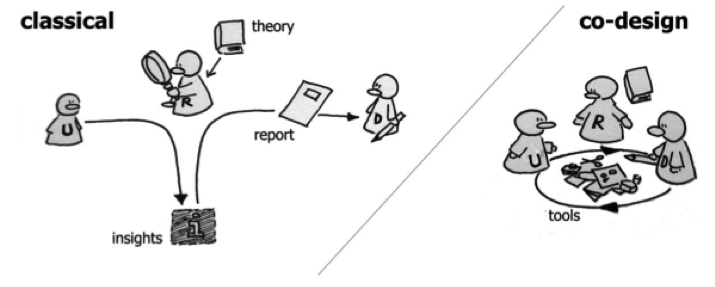
\includegraphics[width=12cm]{Img/CPD/1-CO.png}
\caption[(optional short caption)]{\label{us_figure} Diseño Clásico vs Co-diseño}
\end{figure}

\textcolor{red}{Desarrollar la parte de CAD parametrico y la relacion con CPD}

\begin{figure}
\centering
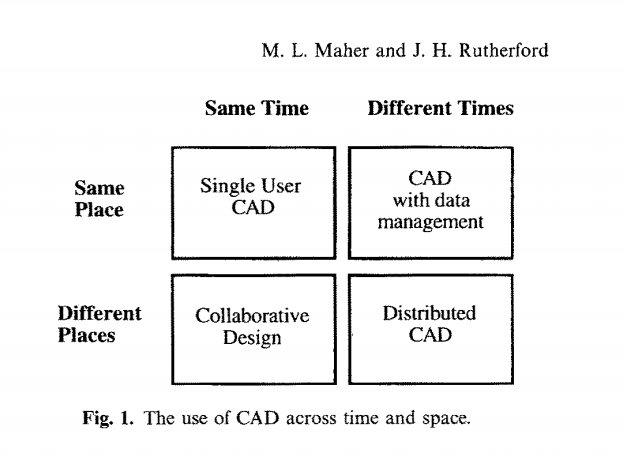
\includegraphics[width=12cm]{Img/CPD/2-CAD.png}
\caption[(optional short caption)]{\label{us_figure} El uso del CAD a través del tiempo y espacio}
\end{figure}


\section{Diseño paramétrico}

El término \textit{paramétrico} se originó en las matemáticas, pero hay un debate sobre cuándo comenzaron los diseñadores a usar la palabra, David Gerber en su tesis doctoral ``Parametric Practice'' acredita a Maurice Ruiter por usar el término en un trabajo de 1988 titulado ``Parametric Design''. En 1987 la compañía Parametric Technology Corporation (PTC), fundada por el matemático Samuel Geisberg lanzó el primer software de modelado paramétrico con éxito comercial: Pro/ENGINEER \footnote{Pro/ENGINEER ahora conocido como Creo Elements/Pro, es un producto de diseño, fabricación e ingeniería asistida por computadora de PTC Corporation (Massachusetts. USA)}. Por su parte, Robert Stiles (2006) sostiene que la verdadera procedencia del término se produjo décadas antes en los escritos de los años 40 por el arquitecto italiano Luigi Moretti.\vskip
Moretti escribió extensamente sobre la arquitectura paramétrica, que define el estudio de los sistemas de arquitectura con el objetivo de \textit{definir las relaciones entre las dimensiones que dependen de los diversos parámetros}. En esa época usó el diseño de un estadio como un ejemplo, explicando cómo la forma del estadio puede derivar de diecinueve parámetros relacionados con aspectos como ángulos de visión y el costo económico del hormigón. Sin embargo, la parametrización tiene una larga historia en las matemáticas y los ejemplos más antiguos que se encontraron para describir modelos tridimensionales se producen mucho tiempo antes. 
Un ejemplo es el artículo de James Dana llamado \textit{On the Drawing of Figures of Crystals} en 1837. En el documento, explica los pasos generales para dibujar una gama de cristales y las disposiciones para sus variaciones utilizando un lenguaje propio mezclado con parámetros, variables y proporciones.\vskip

\begin{figure}
\centering
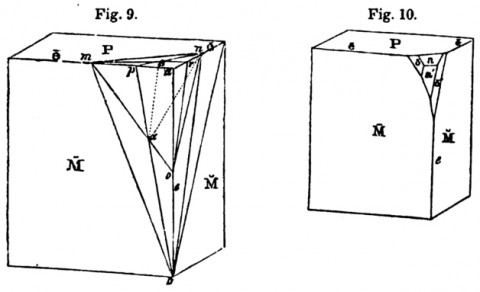
\includegraphics[width=12cm]{Img/CPD/5-DANA.jpg}
\caption[(optional short caption)]{\label{us_figure} DANA}
\end{figure}


Existen muchos otros casos de ciencia del principio del siglo XIX involucrados con las matemáticas de representaciones paramétricas. Un ejemplo de esa época incluye a Sir John Leslie \footnote{John Leslie fué un físico y matemático escocés. Destacó principalmente en el estudio del calor. En 1804 inventó el cubo de Leslie, y en 1810 desarrolló el primer método de congelación artificial.}, en uno de sus libro sobre análisis geométrico, demostrando la auto-similitud de las curvas catenarias usando ``círculos paramétricos''. Otro ejemplo es Samuel Earnshaw. \footnote{Samuel Earnshaw fué un matemático y físico inglés, destacado por sus contribuciones a la física teórica, especialmente el Teorema de Earnshaw.} que escribió sobre ``superficies paramétricas hiperbólicas'' deformadas por líneas de fuerza en un documento que dio lugar al teorema de Earnshaw. Estos ejemplos de expresar la geometría con ecuaciones paramétricas son dos de muchos del período, un período mucho antes de que el arquitecto español Antoni Gaudí\footnote{Antoni Gaudí fué un arquitecto español, máximo representante del modernismo catalán con un sentido innato de la geometría y el volumen \url{http://www.antonigaudi.org/} } comenzara a diseñar arquitectura con curvas catenarias paramétricas y paraboloides hiperbólicos paramétricos a fines del siglo XIX.

Es imposible saber si Gaudí fue influenciado directamente por los científicos y matemáticos que anteriormente utilizaban ecuaciones paramétricas para definir geometrías. 
Mark Burry, el actual arquitecto ejecutivo de "la Sagrada Familia" \footnote{El Templo Expiatorio de la Sagrada Familia, es una basílica católica de Barcelona, diseñada por el arquitecto Antoni Gaudí. Iniciada en 1882, todavía está en construcción.} explica que a pesar de que el currículum universitario de Gaudí incluía, entre otras cosas, matemáticas avanzadas, física general, ciencias naturales y geometría descriptiva ``prácticamente no hay nada escrito por él mismo sobre sus motivaciones, las teorías y las prácticas de su obra''. La comprensión de Gaudí sobre las matemáticas es la base de su arquitectura, especialmente en sus trabajos posteriores, que consiste en superficies diseñadas con helicoides, paraboloides e hiperboloides paramétricamente asociados con superficies regladas, booleanos, relaciones geométricas y arcos catenarios. \cite{Davis2013}

Mark Burry plantea que uno de los primeros ejemplos es la maqueta que utilizó el arquitecto para representar el modelo de la cripta de la Colonia Guell, a principios del siglo XX. Este modelo estaba compuesto por cadenas que sostenían pesos, y actuaban por la fuerza de la gravedad.
La maqueta fue realizada al revés, y Gaudí le sacó una fotografía para poder visualizarla al derecho. Una cadena que cuelga tiene por lo menos cuatro parámetros: su longitud, su peso y los dos puntos a los que está sujetada. La cadena colgando a la merced de la fuerza de la gravedad adopta una forma curva. Esta curva es la función explicita de los parámetros de la cadena, con la propiedad agregada de que cuando es invertida la curva actúa por pura compresión. Al no haber una computadora, la cadena colgante es un modelo paramétrico gracias a la presencia de parámetros que controlan una forma derivada de una función explicita (en este caso, calculada por la gravedad). \cite{Kaled2016}



El \textbf{Diseño Paramétrico} se entiende en términos generales como un proceso de descripción de una problemática utilizando variables. Actualmente para describir estas variables, los diseñadores
insertan valores numéricos o algoritmos en un software especializado, y al cambiar las
variables se generan una serie de alternativas de soluciones, y según el criterio del diseñador, la solución final es creada. Davis (2013) y Hudson (2010) coinciden en que \textit{el diseño paramétrico en su definición contemporánea es únicamente posible creando un \textbf{modelo paramétrico}}. Esto lo definen como un conjunto de ecuaciones que expresan una geometría explícitamente por medio de funciones definidas por parámetros. Esta representación se basa en las relaciones entre estas variables. Todo sistema de esta índole está compuesto por unos parámetros iniciales y las relaciones entre ellos, de manera que si se ajusta uno de los parámetros, el resultado se verá afectado de manera acorde, al igual que si se altera alguna de las relaciones. Esto brinda una característica de fuerte y sencilla maleabilidad, que permite verificar resultados fácilmente. El diseñador que emplea estas herramientas en vez de diseñar un objeto resultante, se enfoca en crear lógicas que pongan en relación estos parámetros y resulten en un sistema vivo y ampliamente modificable de acuerdo al criterio del diseñador, asistido por la
computadora. El uso de este método por medio de la manipulación de los sistemas fomenta la exploración y la experimentación de las formas del producto, que se generan automáticamente por la modificación de los parámetros o las relaciones. Woodbury (2010) afirma que el diseño es cambio y que el modelado paramétrico representa el cambio. Esto lo menciona como una característica esencial del diseño paramétrico, como aquello que lo distingue de los métodos de diseño tradicionales. Es marcar e identificar las partes y como se relacionan y cambian de manera coordinada. (Woodbury, 2010). La demostración explicita de las partes es lo que contribuye a la intervención y modificación
interactiva en tiempo real, debido a la operatividad visible del cambio en el sistema. La
lógica sistemática del diseño paramétrico permite evaluar las relaciones de manera visible, en lugar de hacerlo de manera intuitiva por medio de un proceso mental interno.
Esto le permite al diseñador explorar y descubrir nuevas posibilidades en lugar de hurgar en sus conocimientos previos para llegar con una solución que ya conocía (Cross, 2006).
El autor también afirma que es necesaria una representación visual ya que diseñar es difícil de conducir puramente por procesos mentales internos (Cross, 2011, p. 12).\vskip
 


\begin{figure}
\centering
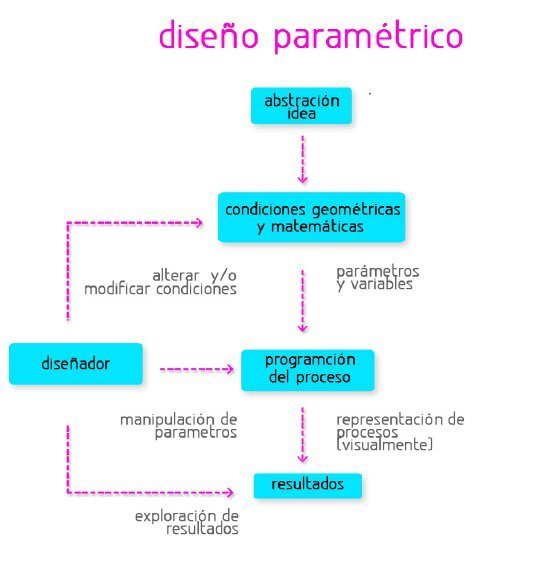
\includegraphics[width=12cm]{Img/CPD/4-PARAM.jpg}
\caption[(optional short caption)]{\label{us_figure} Proceso de diseño paramétrico }
\end{figure}


\subsection{CAD Paramétrico}

La innovación del modelo de Gaudí explicado en el punto 2.1.4 radica en que este calcula automáticamente los resultados, ya que al mover un parámetro se afecta todo el modelo, que a pesar de ser análogo, marcó el inicio de la actualización en tiempo real de geometrías con bases matemáticas, lo cuál le da el énfasis utilitario de explorar las
posibilidades que el modelo ofrece (ver Figura 1, pg. 95, anexo de imágenes seleccionadas).
Esto marcó la \textit{necesidad de facilitar la interacción entre el diseñador y el modelo}, que implicaba muchas representaciones manuales y modificaciones completas con cada cambio. No fue hasta la aparición de las computadoras y el primer programa CAD, 29 Sketchpad de Ivan Sutherland en 1963 que se facilitó la interacción en tiempo real del diseñador y la computadora. Yüksel lo describe como un sistema que tenía un puerto de entrada con un modelo de límites que promovía la interacción, porque al manipular una parte del modelo afectaría los cambios geométricos en otro. En el contexto de aparición de este programa, el proceso de diseño era enteramente manual y análogo, donde un cambio mínimo significaría comenzar de nuevo. Al representar las geometrías en dos dimensiones en la computadora se facilitaba el proceso de diseño. A partir de esto se fueron desarrollando un amplio número de software cuyas capacidades y posibilidades se extendían con aquellas del procesamiento de datos de las
computadoras.
El recorrido histórico del desarrollo de software excede los objetivos de este trabajo final, pero la bifurcación entre el diseño computacional y la computarización del diseño es esencial para la compresión de los capítulos a seguir. Ambos términos suelen ser tomados como iguales, definidos como el uso de tecnologías CAD para realizar un
proyecto de diseño. La diferencia radica en su empleo. \vskip
La computarización del diseño apunta a el uso de la computadora como herramienta de dibujo o representación formal de un proyecto concebido en la mente del diseñador, mientras que el diseño computacional aborda el diseño con bases en el pensamiento algorítmico, lo que engloba al diseño paramétrico y generativo. Esta diferenciación puede apreciarse claramente en el modelo de Gaudí y Sketchpad, el programa de Sutherland. La maqueta de Gaudí encarna un sistema de complejo de parámetros y relaciones, mientras que Sketchpad representa geometrías modificables. \cite{Kaled2016}


Un ejemplo de software paramétrico masivamente utilizado es FreeCAD\footnote{\url{https://www.freecadweb.org/}}, una aplicación FLOSS de CAD en tres dimensiones e ingeniería asistida por computadora para la asistencia en ingeniería mecánica y el diseño de elementos mecánicos. Está basado en Open CASCADE y programado en los lenguajes C++ y Python. Utiliza técnicas de modelado paramétrico y está provisto de una arquitectura de software modular, permitiendo añadir funcionalidades mediante el lenguaje python sin tener que cambiar el núcleo del sistema.

\textcolor{red}{
En este trabajo se utiliza el concepto de diseño computacional con la utilización de modelos 3D paramétricos como medio para lograr la colaboración. Es indispensable que los diseños se generen en función de sus parámetros y además expongan sus características de manera comprensible por todas las partes involucradas. Por ejemplo: un diseñador industrial puede comprender naturalmente parámetros como arista, vértices o normales pero un artista puede comprender sobre dimensiones, colores o materiales. Por ende es recomendable que los modelos 3D en este caso se expongan en función de los parámetros conocidos por el artista.
Para ello surge la necesidad de mecanismos de manipulación directa de los modelos 3D por parte de los interesados para posibilitar la generación de nuevas soluciones, y así gracias al diseño iterativo lograr la colaboración.}



\subsection{CAD Paramétrico especificado en algoritmos} 
El diseño paramétrico también es posible a través de las interfaces de secuencias de comandos del inglés \textit{scripting}\footnote{Un script es un programa informático usualmente simple, que por lo general se almacena en un archivo de texto plano. }. Las interfaces de scripting permiten a los diseñadores escribir código para automatizar partes del software. Los desarrolladores de software como AutoCAD\footnote{AutoCAD es un software de CAD utilizado para dibujo 2D y modelado 3D, Desarrollado y comercializado por la empresa Autodesk.}, incluso en 1982, se dieron cuenta de que la inclusión de estas interfaces les permitía ``Evitar muchas cosas personalizadas de codificación y aplicación que de lo contrario se les pediría". Diez años más tarde, en 1992, cuando Mark Burry\footnote{Mark Cameron Burry es un arquitecto neozelandés y profesor de Arquitectura del Royal Melbourne Institute of Technology en Melbourne.} quería modelar las hipérbolas paramétricamente para la Sagrada Familia, en lugar de pedirle a la empresa Autodesk que incluyera una función de hipérbola en AutoCAD, utilizó la interfaz de scripting para desarrollar una propia. El script de Burry tenía tres parámetros de entrada: un punto de origen, un punto mínimo y un punto de asíntota. Estos parámetros se alimentan a través de una serie de ecuaciones explícitas escritas en código AutoLISP\footnote{AutoLISP es un lenguaje de programación derivado del lenguaje Lisp. Es utilizado para generar rutinas en AutoCAD y sus derivados.} para emitir una hipérbola. 

El script, con sus parámetros de entrada, funciones explícitas y salidas es una realización arquetípica de la definición matemática de paramétrico. Ipek Dino \cite{Dino2012} ha argumentado que los scripts son inherentemente paramétricos, señalando que \textit{``los sistemas paramétricos se basan principalmente en principios algorítmicos ya que un algoritmo toma un valor o un conjunto de valores como entrada, ejecuta una serie de pasos computacionales que transforman la entrada y finalmente produce un valor o un conjunto de valores como salida".}
\vskip Por lo tanto, las interfaces de scripting accesibles en la mayoría de los paquetes de software están naturalmente predispuestas a crear modelos paramétricos.

Estas interfaces se puede encontrar en programas como OpenSCAD\footnote{http://www.openscad.org/}. OpenSCAD es una aplicación FLOSS para crear objetos sólidos de CAD utilizando geometría constructiva de sólidos (CSG). No es un editor interactivo sino un compilador 3D basado en un lenguaje de descripción textual. Un documento de OpenSCAD especifica primitivas geométricas y define como son modificadas y manipuladas para reproducir un modelo 3D.



En la última década se ha visto la aparición de un nuevo tipo de interfaz de secuencias de comandos, la interfaz visual. La programación visual implica representar programas no como texto, sino como diagramas. Un ejemplo es Grasshopper \footnote{Grasshoper es un editor visual de algoritmos integrado en el software Rhino 3-D. \url{http://www.grasshopper3d.com/}} que se basa en gráficos (un nombre matemático para un tipo de diagrama de flujo) que mapean el flujo de relaciones desde parámetros, a través de funciones definidas por el usuario, concluyendo normalmente con la generación de geometría. Los cambios en los parámetros o las relaciones del modelo hacen que los cambios se propaguen a través de las funciones explícitas para volver a dibujar automáticamente la geometría. Como tal, son otra forma de crear un modelo paramétrico.



VENTAJAS TECNICAS DE USAR CODIGO EN LOS MODELOS

http://www.patrikschumacher.com/Texts/Design%20Parameters%20to%20Parametric%20Design.html

http://fernandoalonsoarchitect.blogspot.com.ar/2017/01/historia-del-diseno-parametrico.html

Las herramientas de diseño asistido por computadora CAD tradicionales fueron pensadas para un usuario, por ende tienen limitaciones para soportar el entorno de desarrollo colaborativo de productos CPD y de forma rápida como requiere el mercado. Actualmente el desarrollo de productos es el resultado de procesos colaborativos basados en la red, porque la mayoría de los proyectos requieren la cooperación entre actores distribuidos geográficamente. En un proceso de desarrollo distribuido, se necesita una comunicación efectiva y de alta velocidad. La mayoría de los errores de diseño se deben a la falta de comunicación entre los equipos de diseño distribuidos.
Los sistemas de información distribuída que se han aplicado para CPD se pueden clasificar en 3: web services, remote services y remote repositories.Los sistemas basados en web services tienen ventajas sobre los otros dos porque son relativamente sencillos de diseñar e implementar, reducen los problemas de la instalación de software y facilita la posibilidad de la colaboración. \cite{Nyamsuren2015}



Articulo: Collaborative 3D Workspace and Interaction Techniques
for Synchronous Distributed Product Design Reviews. 
Emergence in collaborative computer-aided design

\section{Modelado Geométrico}


http://di002.edv.uniovi.es/~rr/Tema7.pdf

Los modelos son útiles, dado que a menudo permiten hacer estudios
sobre objetos que de otra forma sería difícil realizar, ya sea porque aún no
existen (aviones, barcos, etc.), o por que no son observables directamente
(moléculas). Sin embargo, los modelos físicos y matemáticos están limitados
al ámbito de su utilidad, de forma que para analizar un nuevo problema
normalmente se requiere un nuevo modelo. Se ha intentado paliar este inconveniente
dando a los modelos un carácter de generalidad. Tradicionalmente ha sido el dibujo técnico quien mayor éxito ha tenido como técnica de
propósito general para describir modelos, ya que los planos se pueden utilizar para extraer información de diversas clases, incluyendo los datos para la formación de modelos físicos y matemáticos.
Sin embargo, con la llegada de los sistemas informáticos el dibujo técnico ha sido desplazado por los \textit{modelos informáticos}, que debido a su dinamismo y universalidad superan con creces a cualquier otro tipo de modelado.\vskip


Los modelos informáticos se sirven de la enorme potencia de procesado de los ordenadores para realizar tareas similares a las que podrían hacerse con los modelos mencionados anteriormente, pero intentando aprovechar sus ventajas y evitar sus inconvenientes. Mediante técnicas y algoritmos desarrollados formalmente, es decir, con una base matemática sólida, se consiguen sistemas de modelado de propósito general que soportan una gran variedad de modelos diferentes, de igual modo que el dibujo técnico.\vskip

La cantidad total de datos que se deben almacenar en un modelo informático, depende del ámbito de las preguntas que algorítmicamente queramos responder a partir del modelo.
Muchos de los problemas a resolver mediante modelos tienen naturaleza geométrica.
Por ejemplo, el problema de hallar la imagen coloreada de un
objeto incluye cuestiones geométricas tales como:\vskip
a) ¿Qué partes del objeto son visibles para el observador?\vskip
b) ¿Qué color ha de ser asignado a cada punto de la imagen? \vskip

Si podemos representar en el ordenador la forma geométrica de un objeto,
podremos responder a estas preguntas y a muchas otras. De hecho, la
información geométrica sobre un objeto es la parte \textcolor{red}{más útil} del total de información
sobre el objeto. Además, las técnicas para almacenar y procesar la
información geométrica son relativamente independientes de un modelo
particular. Así, procesos esencialmente iguales de modelado se utilizan en la
construcción de modelos de barcos, casas, o zapatos.
Acorde con lo dicho anteriormente, en un modelo tiene sentido separar
la información geométrica de los objetos, de la no geométrica. Bajo este
planteamiento, al total de información del modelo informático se conoce como
modelo del objeto, mientras que la información exclusivamente geométrica
constituye el modelo geométrico.\vskip

Por lo tanto, el concepto de Modelado Geométrico se refiere al conjunto de métodos utilizados para definir la forma y otras características de los objetos. La construcción de los objetos es normalmente, en si misma, una operación asistida por ordenador. Éstos juegan un papel primordial, ya que sin su potencia de cálculo los procedimientos del Modelado Geométrico solamente podrían aplicarse en modelos de escasa importancia práctica.
Los métodos del Modelado Geométrico vienen a ser un compendio de las técnicas utilizadas en varias disciplinas, como la Geometría Analítica y Descriptiva, la Topología, la Teoría de Conjuntos, el Análisis Numérico, las Estructuras de Datos, el Cálculo Vectorial y los Métodos Matriciales.\vskip
Se pueden enumerar tres aplicaciones básicas del Modelado Geométrico: 

\begin{itemize}
  \item Representación de los objetos existentes.
  \item Diseño de los objetos inexistentes y
  \item Visualización (rendering) de los objetos.
\end{itemize}
\vskip

El CAD y el CAM, han sido las principales fuerzas de desarrollo del campo del Modelado Geométrico, aunque otras áreas como la Robótica, Reconocimiento de Formas, Inteligencia Artificial, y el Cálculo Estructural (modelos de elementos finitos) han contribuido también ha su desarrollo.

\subsection{Transformaciones geométricas }

El conjunto de operaciones elementales que realiza internamente un computador para conseguir pasar de la representación de un modelo geométrico tridimensional a su imagen en pantalla 2D, pero que para la impresión del observador parezca estar contemplando un sistema de visualización en el mundo real con tres dimensiones 3D, utiliza las transformadas geométricas. 
Existen varias transformaciones geométricas, en este trabajo se revisan el escalamiento, la translación y la rotación.

\subsubsection{Representación}

En el área de la graficación por computadora, es común encontrar la representación de las ecuaciones de trasformación por medio de matrices, y se pueden encontrar dos tipos de notaciones para representarlas, una es representando las coordenadas de un punto \textit{p} como \textit{vectores renglón}, en este caso una matriz de transformación \textit{M} en 2D, multiplica al punto por la derecha para obtener el nuevo punto \textit{p'}.

$$ p = \begin{bmatrix}
       x_{1} & x_{2}         
     \end{bmatrix}, \ p^{\prime} = \begin{bmatrix}
       x_{1} & x_{2}         
     \end{bmatrix}= p.M $$
     
La segunda notación es representando las coordenadas de un punto \textit{p} como \textit{vectores columna}, en este caso una matriz de transformación \textit{M}, multiplica al punto por la izquierda para obtener el nuevo punto \textit{p'}.

$$ p = \begin{bmatrix}
       x_{1} \\ x_{2}         
     \end{bmatrix}, \ p^{\prime} = \begin{bmatrix}
       x_{1} \\ x_{2}           
     \end{bmatrix}= p.M $$
     
En este trabajo, se representan los puntos por medio de \textit{vectores renglón}, por lo tanto las matrices de transformación estarán modeladas para multiplicarlas por la derecha, sin embargo se puede obtener una matriz de transformación en la otra notación calculando su transpuesta.
No todas las transformaciones son aplicadas a un punto como una multiplicación de
factores, por tal razón se utilizan las \textit{coordenadas homogéneas} para la representación matricial, y de esta forma todas las transformaciones son tratadas como multiplicaciones.
En coordenadas homogéneas, a cada punto 2D se le agrega una tercera coordenada, de esta forma, en lugar de representar los puntos como $p = (x_{1},\ x_{2}) $  son representados como la terna $p = (x_{1},\ x_{2},\ \omega)$ , al mismo tiempo se dice que un par de coordenadas homogéneas $ (x_{1},\ x_{2}) $ y $(x_{1},\ x_{2},\ \omega)$ representan el mismo punto si una es múltiplo de la otra. Por ejemplo, la terna (4, -2, 6) y (8, -4, 12) representan el mismo punto 2D pero en diferentes coordenadas triples, esto significa que cada punto tiene un sinfín de representaciones en coordenadas homogéneas.\vskip
Al menos una de las coordenadas homogéneas tiene que ser distinta de cero, por lo tanto la terna (0, 0, 0) no es válida. Si la coordenada $\omega \neq 0$, la terna $(x_{1},\ x_{2},\ \omega)$ se puede dividir entre $\omega$ y se obtiene $(x_{1}/\omega,\ x_{2}/\omega,\ 1)$ , cuando se realiza esta división, a los valores $x_{1}/ \omega$ y  $x_{2}/ \omega$  se les llama \textit{coordenadas cartesianas} del punto homogéneo. Una
elección conveniente es hacer el valor de
$\omega = 1$, así cada posición 2D es representada con las coordenadas homogéneas $(x_{1}/\omega,\ x_{2}/\omega,\ 1)$. \vskip
En general para cualquier dimensión las coordenadas homogéneas de un punto \textit{p} en \textit{n}D se escribe como $p = (x_{1},\ x_{2},...,x_{2},\omega)$, el cuál es un vector de longitud \textit{n}+1.


\subsubsection{Extensión de las Transformaciones a Otras Dimensiones}
Las trasformaciones geométricas 3D son extensiones de las transformaciones geométricas 2D, pero con la incorporación del eje Z. Muchas de las operaciones matemáticas utilizadas en las transformaciones de escalamiento y translación se extienden fácilmente, pero la rotación no es tan intuitiva y requiere de un poco más de análisis, para comprender su generalización a otras dimensiones y facilitar su comprensión se explica mas adelante la rotación 2D.

\subsubsection{Escalamiento 3D}
El escalamiento permite cambiar el tamaño de un objeto expandiéndolo o
contrayéndolo en sus dimensiones.
El escalamiento 3D implica el cambio de tamaño de un poliedro, donde cada punto $p = (x_{1},\ x_{2},\ x_{3})$ es transformado por la multiplicación de tres factores de escalamiento: $s_{1}, s_{2}$ y $s_{3}$ a lo largo de los ejes $X_{1},\ X_{2},\ X_{3}$ respectivamente, de esta forma, las coordenadas del nuevo punto $p^{\prime} = (x_{1}^{ \prime},\ x_{2}^{ \prime},\ x_{3}^{ \prime})$ se obtienen como:

$$x_{1}{\prime} = x_{1}.s_{1}$$
$$x_{2}{\prime} = x_{2}.s_{2}$$
$$x_{3}{\prime} = x_{3}.s_{3}$$

Sea $s = (s_{1},\ s_{2},\s_{3})$ el vector de factores de escalamiento, y $S(s)$ la matriz de
escalamiento, en coordenadas homogéneas el escalamiento de un punto $p$ en 3D se puede expresar como el producto matricial
$p^{\prime} = p.S(s)$ , es decir:

$$
\begin{array}{rccl}
\left[
\begin{array}{rccl}
x_{1}{\prime} & x_{2}{\prime} & x_{3}{\prime} & 1\\
\end{array}
\right]
\end{array}
=
\begin{array}{rccl}
\left[
\begin{array}{rccl}
x_{1} & x_{2} & x_{3} & 1\\
\end{array}
\right]
\end{array} 
.
\left[
\begin{array}{rccl}
s_{1} & 0 & 0 & 0\\
0 & s_{2} & 0 & 0\\
0 & 0 & s_{3} & 0\\
0 & 0 & 0 & 1\\
\end{array}
\right]
$$

\begin{center}
\textbf{\footnotesize{Expresión matricial para el escalamiento 3D.}}
\end{center}

\begin{figure}[h]
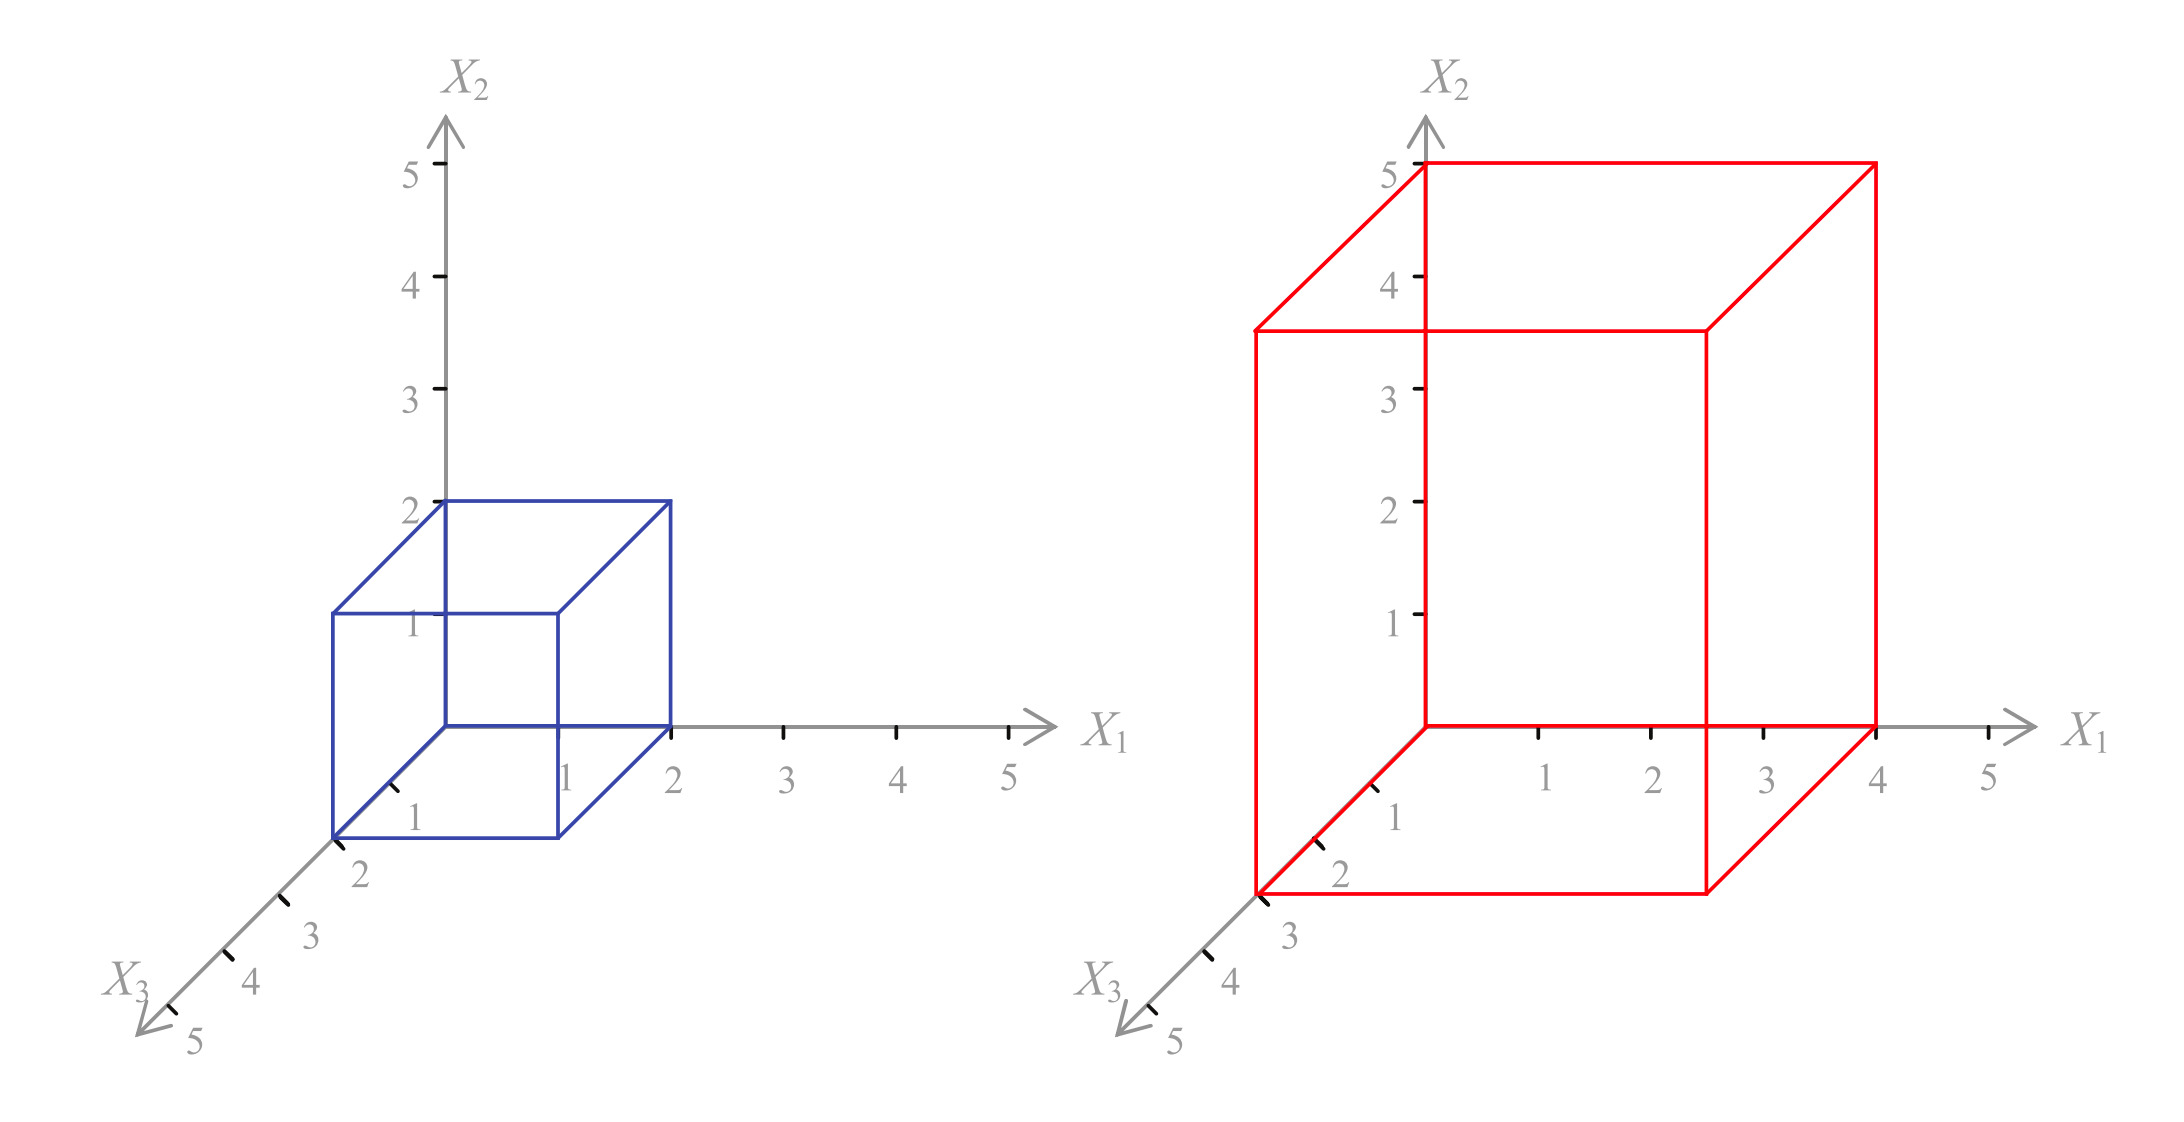
\includegraphics[width=12cm]{Img/GEO/geo-escala.jpg}
\centering
\end{figure}

La Figura muestra el efecto de escalamiento de una figura con $s1$ = 2, $s2$ = 2.5 y $s3$ = 1.5.

\subsubsection{Traslación 3D}
La translación permite desplazar un objeto a lo largo de sus dimensiones, como resultado se obtiene un cambio de posición. La translación 3D implica el desplazamiento de un poliedro, donde cada punto $p = (x_{1},\ x_{2},\ x_{3})$ es trasladado $d1$ unidades en el eje $X_1$ , $d_2$ unidades en el eje $X_2$ y $d_3$ unidades en el eje $X_3$, de esta forma, las coordenadas del nuevo punto
$p^{\prime} = (x_{1}^{\prime},\ x_{2}^{\prime},\x_{3}^{\prime})$ se obtienen como:

$$x_{1}^{\prime} = x_{1} + d1$$
$$x_{2}^{\prime} = x_{2} + d1$$
$$x_{3}^{\prime} = x_{3} + d1$$

Sea $d = (d_{1},\ d_{2},\ d_{3})$ el vector de distancias, y $T(d)$ la matriz de translación, en
coordenadas homogéneas la translación de un punto $p$ en 3D se puede expresar como el producto matricial $p^{\prime} = p + T(d)$ , es decir:

$$
\begin{array}{rccl}
\left[
\begin{array}{rccl}
x_{1}{\prime} & x_{2}{\prime} & x_{3}{\prime} & 1\\
\end{array}
\right]
\end{array}
=
\begin{array}{rccl}
\left[
\begin{array}{rccl}
x_{1} & x_{2} & x_{3} & 1\\
\end{array}
\right]
\end{array} 
.
\left[
\begin{array}{rccl}
1 & 0 & 0 & 0\\
0 & 1 & 0 & 0\\
0 & 0 & 1 & 0\\
d_{1} & d_{2} & d_{3} & 1\\
\end{array}
\right]
$$

\begin{center}
\textbf{\footnotesize{Expresión matricial para la traslación 3D.}}
\end{center}

La Figura 3.4 muestra el efecto de translación de una figura con $d1$ = 2, $d2$ = 0 y $d3$ = 2.

\begin{figure}[h]
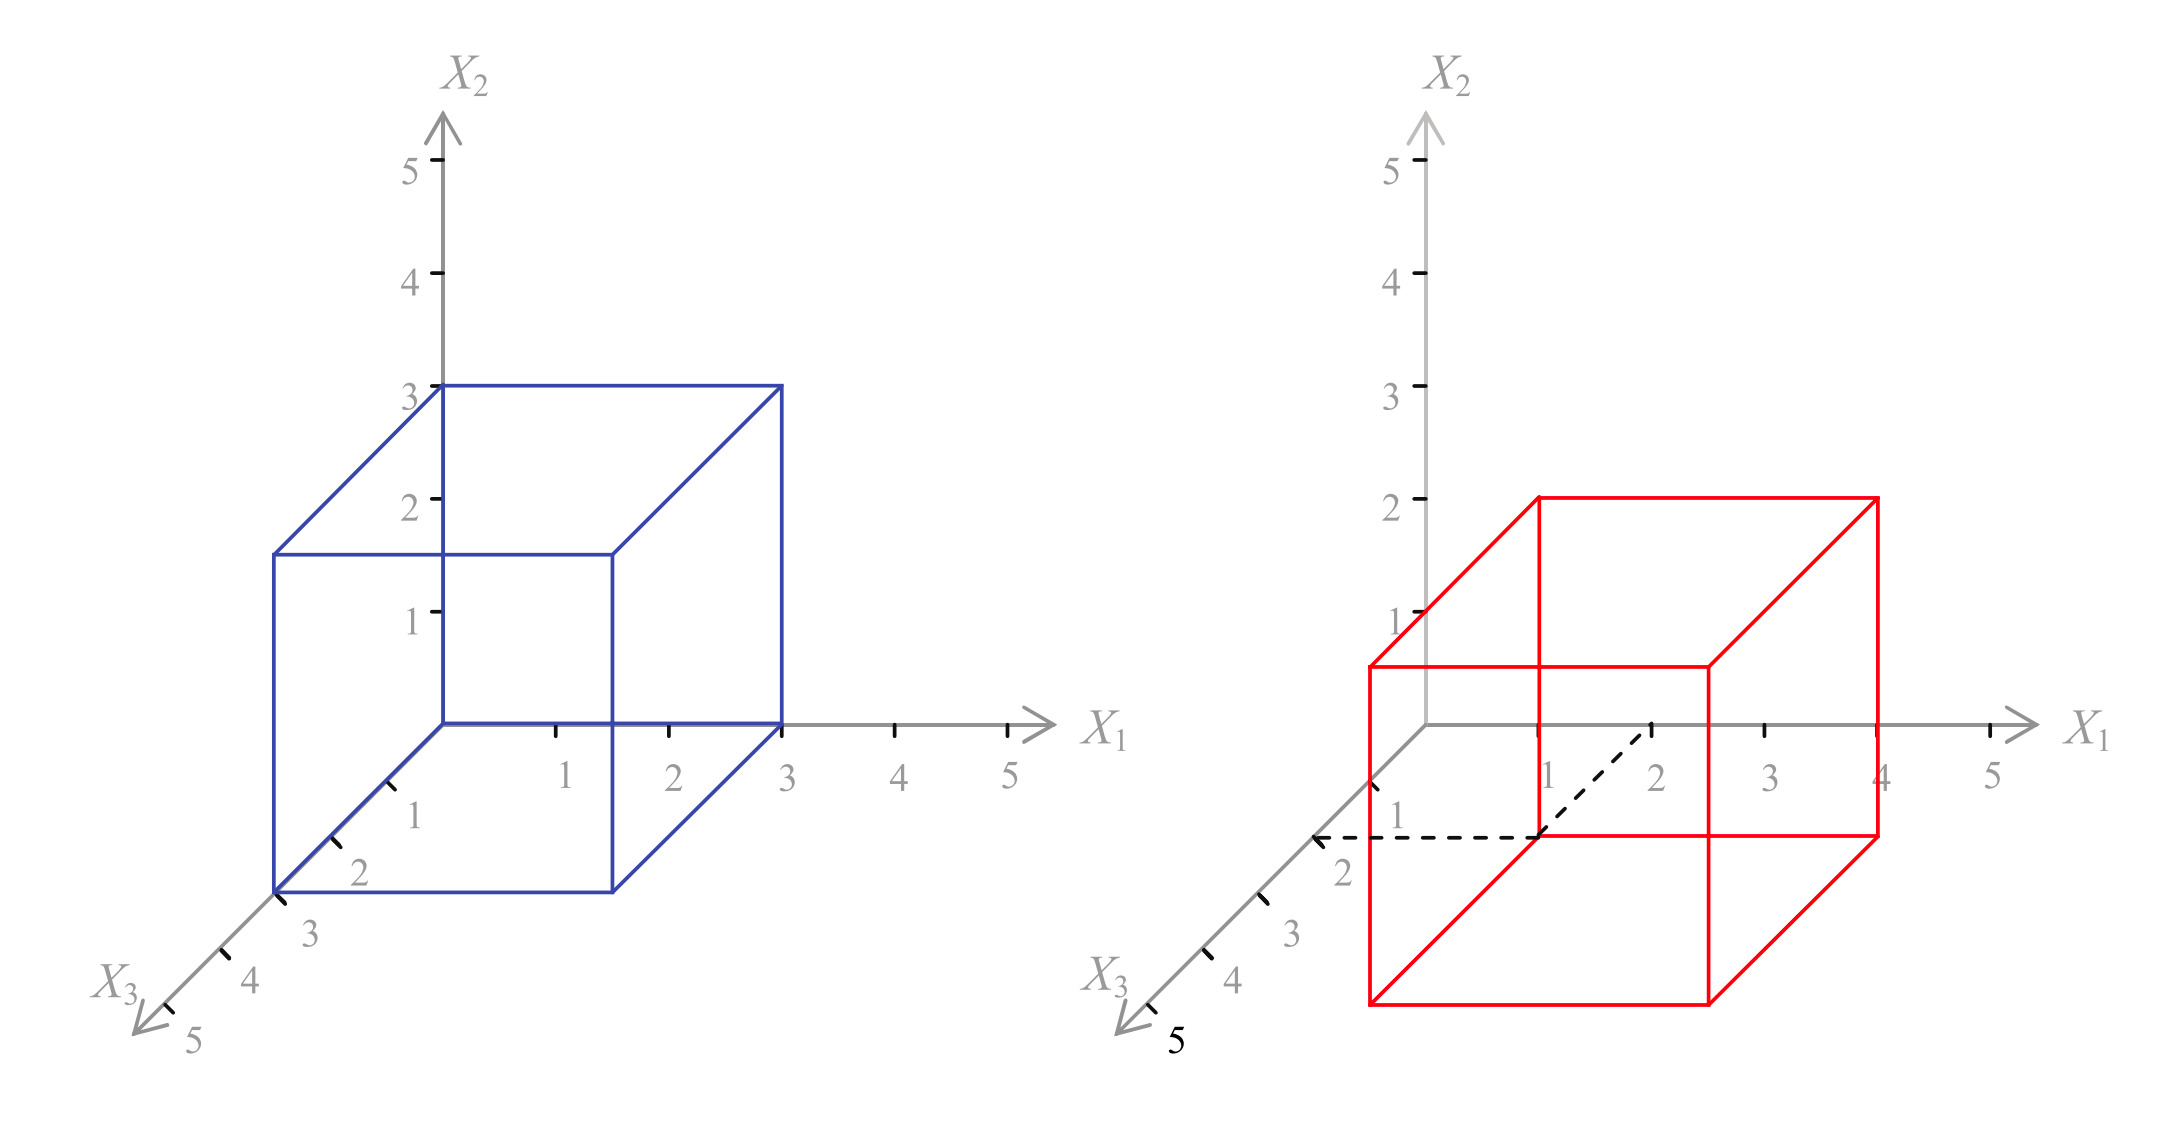
\includegraphics[width=12cm]{Img/GEO/geo-traslacion.jpg}
\centering
\end{figure}

\subsubsection{Rotación 2D}
La rotación permite girar un objeto sobre un eje de rotación, dado un valor de ángulo de rotación $\theta$ y su dirección. La rotación de un objeto en 2D se lleva a cabo alrededor de un punto, que es el eje
puntual (cero-dimensional) de rotación.\vskip
Para generar una rotación, se especifica el ángulo de rotación , y el punto de rotación $\theta$ (pivote) sobre el cuál el objeto será rotado. Los ángulos de rotación positivos definen una rotación en sentido contrario a las agujas del reloj o sentido antihorario sobre el punto pivote (del eje $X_1$ al eje $X_2$), entonces los ángulos de rotación negativos producen una rotación en el sentido de las agujas del reloj o sentido horario (del eje $X_2$ al eje $X_1$). La rotación 2D es el giro sobre el eje de rotación que es perpendicular al plano $X_1 X_2$ (mejor conocido como plano XY) y que pasa a través del punto pivote.\vskip
Si el punto pivote se encuentra sobre el origen, se tiene que: $r$ es la distancia del punto $p = (x_{1}, \ x_{2})$ al origen, $\phi$ define la posición angular del punto p desde la horizontal, y θ el ángulo de rotación de $p$ para producir el nuevo punto $p^{\prime} = ({x_{1}}^{\prime},\ {x_{2}}^{\prime})$

\begin{center}
\begin{figure}[h]
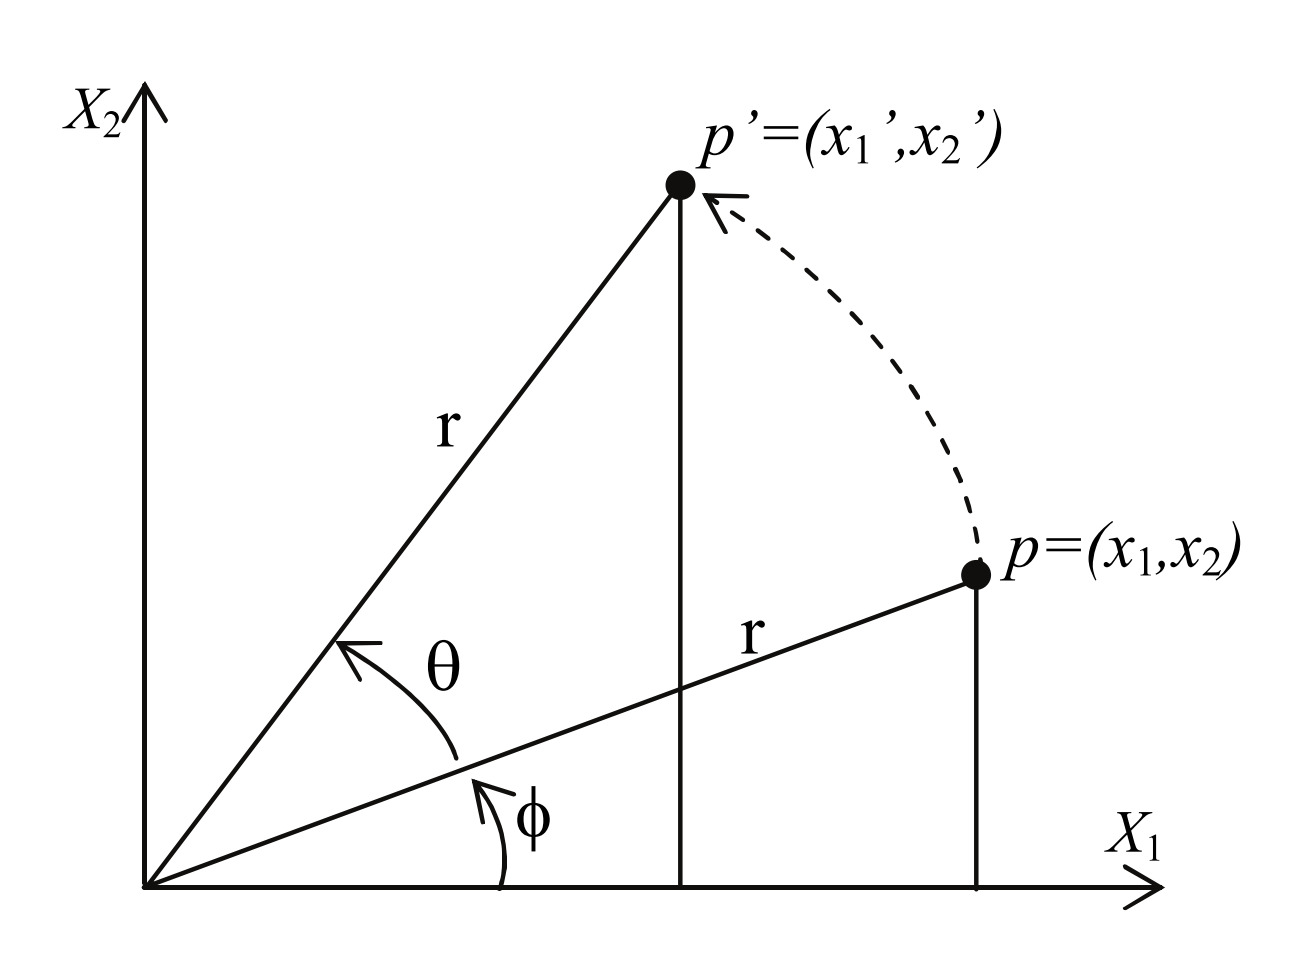
\includegraphics[width=8cm]{Img/GEO/geo-rotacion2d.jpg}
\centering
\caption{\textbf{\footnotesize{Rotación de un punto en 2D alrededor del origen.}}}
\end{figure}
\end{center}

Utilizando coordenadas polares, el punto $p = (x_{1}, \ x_{2})$ se puede escribir como $p = (r, \ \phi)$ y el punto $p^{\prime} = ({x_{1}}^{\prime},\ {x_{2}}^{\prime})$ como $p^{\prime} = (r, \ \phi + \theta)$. Pasando después estos puntos de coordenadas polares a rectangulares se tiene que:

$$
\begin{array}{rccl}
x_{1} = r \cos(\phi)  & x_{2} = r \sin(\phi)\\
{x_{1}}^{\prime} = r \cos(\phi + \theta)  & {x_{2}}^{\prime} = r \sin(\phi + \theta)
\end{array}
$$

Aplicando algunas propiedades trigonométricas:
$$
{x_{1}}^{\prime} = r \cos(\theta + \phi) = r \cos \phi \cos \theta - r \sin \phi \sin \theta
$$
$$
{x_{2}}^{\prime} = r \sin(\theta + \phi) = r \cos \phi \cos \theta - r \sin \phi \sin \theta
$$

Substituyendo los valores de $x_{1} = r \cos(\phi)$ y $x_{2} = r \sin(\phi)$ se obtienen las ecuaciones para rotar un punto $p = (x_{1}, \ x_{2})$ alrededor del origen dado un ángulo $\theta$

$$
\begin{cases}
{x_{1}}^{\prime} = x_{1} \cos(\theta) -x_{2} \sin(\theta) \\ 
{x_{2}}^{\prime} = x_{1} \sin(\theta) -x_{2} \cos(\theta)
\end{cases}
$$

\begin{center}
\textbf{\footnotesize{Fórmulas para la rotación 2D alrededor del origen.}}
\end{center}

Sea $R(\theta)$ la matriz de rotación sobre el origen, en coordenadas homogéneas la
rotación de un punto p alrededor del origen en 2D se puede expresar como el producto matricial $p^{\prime} = p.R(\theta)$, es decir:

$$
\begin{array}{rccl}
\left[
\begin{array}{rccl}
x_{1}{\prime} & x_{2}{\prime} & 1\\
\end{array}
\right]
\end{array}
=
\begin{array}{rccl}
\left[
\begin{array}{rccl}
x_{1} & x_{2} &  1\\
\end{array}
\right]
\end{array} 
.
\left[
\begin{array}{rccl}
\cos\theta & \sin\theta & 0\\
-\sin\theta & \cos\theta & 0\\
0 & 0 & 1\\
\end{array}
\right]
$$

\begin{center}
\textbf{\footnotesize{Expresión matricial para la rotación 2D.}}
\end{center}

\begin{figure}[h]
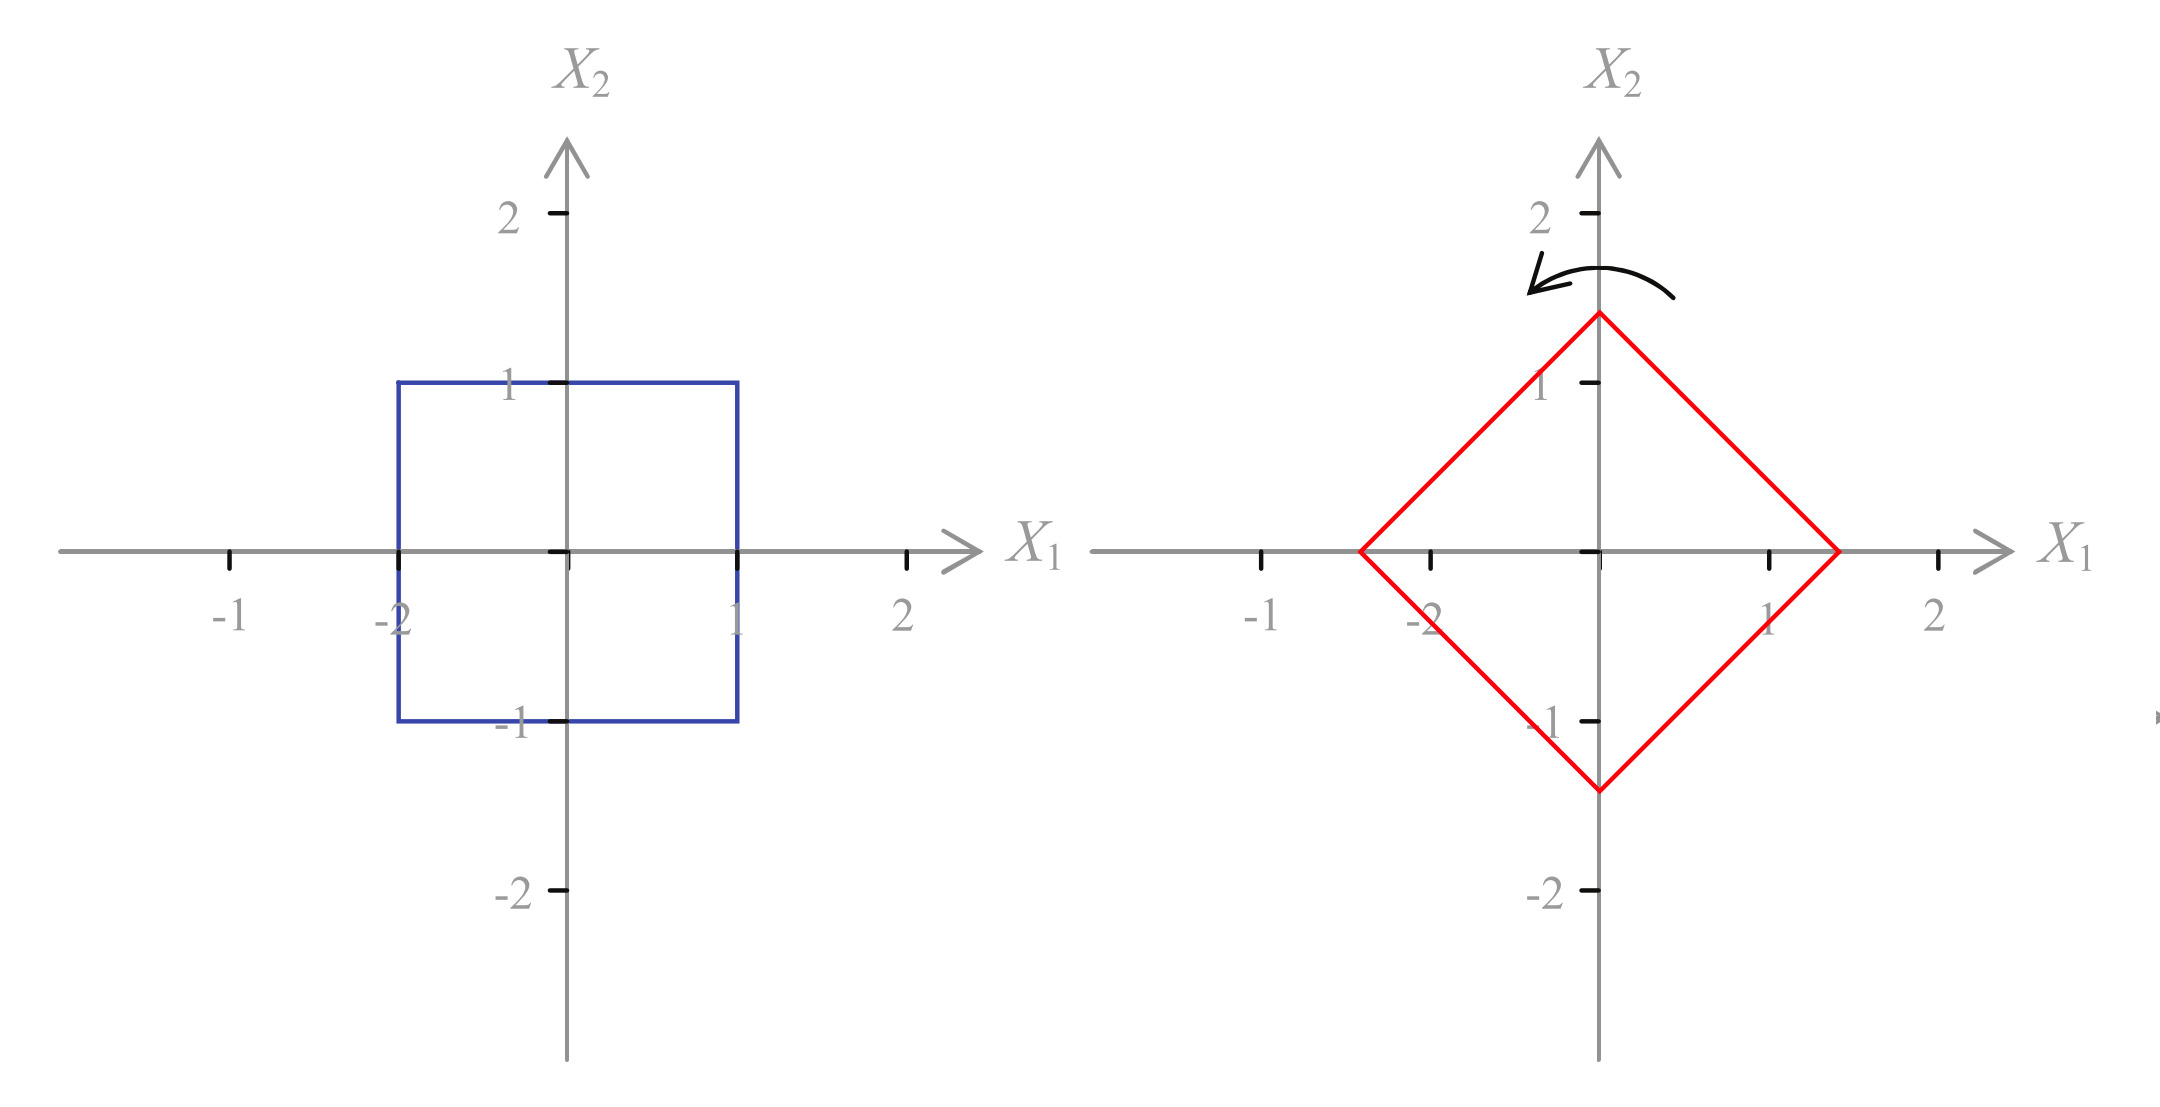
\includegraphics[width=12cm]{Img/GEO/geo-rotacion2d45.jpg}
\centering
\caption{\textbf{Ejemplo de rotacion 2D con $\theta = 45^{\circ}$}}
\end{figure}



\subsubsection{Rotaciones principales 3D}

A diferencia de la rotación en el espacio 2D\cite{Matias2007}, donde para hacer rotar un objeto se necesita un punto (cero-dimensional), en 3D para hacer rotar un objeto se necesitan dos puntos no coincidentes que determinan un segmento de recta, cuya línea de soporte define un eje lineal (uni-dimensional) de rotación.\vskip
Las \textit{rotaciones principales} 3D, son aquellas cuando el eje de rotación se encuentra sobre alguno de los tres ejes principales: $X_{1}$, $X_{2}$ o $X_{1}$, las rotaciones sobre cualquier otro eje arbitrario son llamadas \textit{rotaciones generales} 3D. Se recuerda que inicialmente, se analizan las rotaciones principales.
Por convención, los ángulos de rotación positivos producen rotaciones en contra de
las agujas del reloj (antihorario) sobre el eje de rotación, esto es si se observa el giro desde la parte positiva del eje hacia el origen. Otra forma de determinar la dirección de un giro positivo es mediante la \textbf{regla de la mano derecha} (Figura 3.7), que dice que: \textit{“Si se coloca el dedo pulgar de la mano derecha sobre el eje de rotación apuntando hacia la parte positiva de dicho eje, el giro natural del resto de los dedos indica la dirección positiva del giro”.}

\begin{figure}[h]
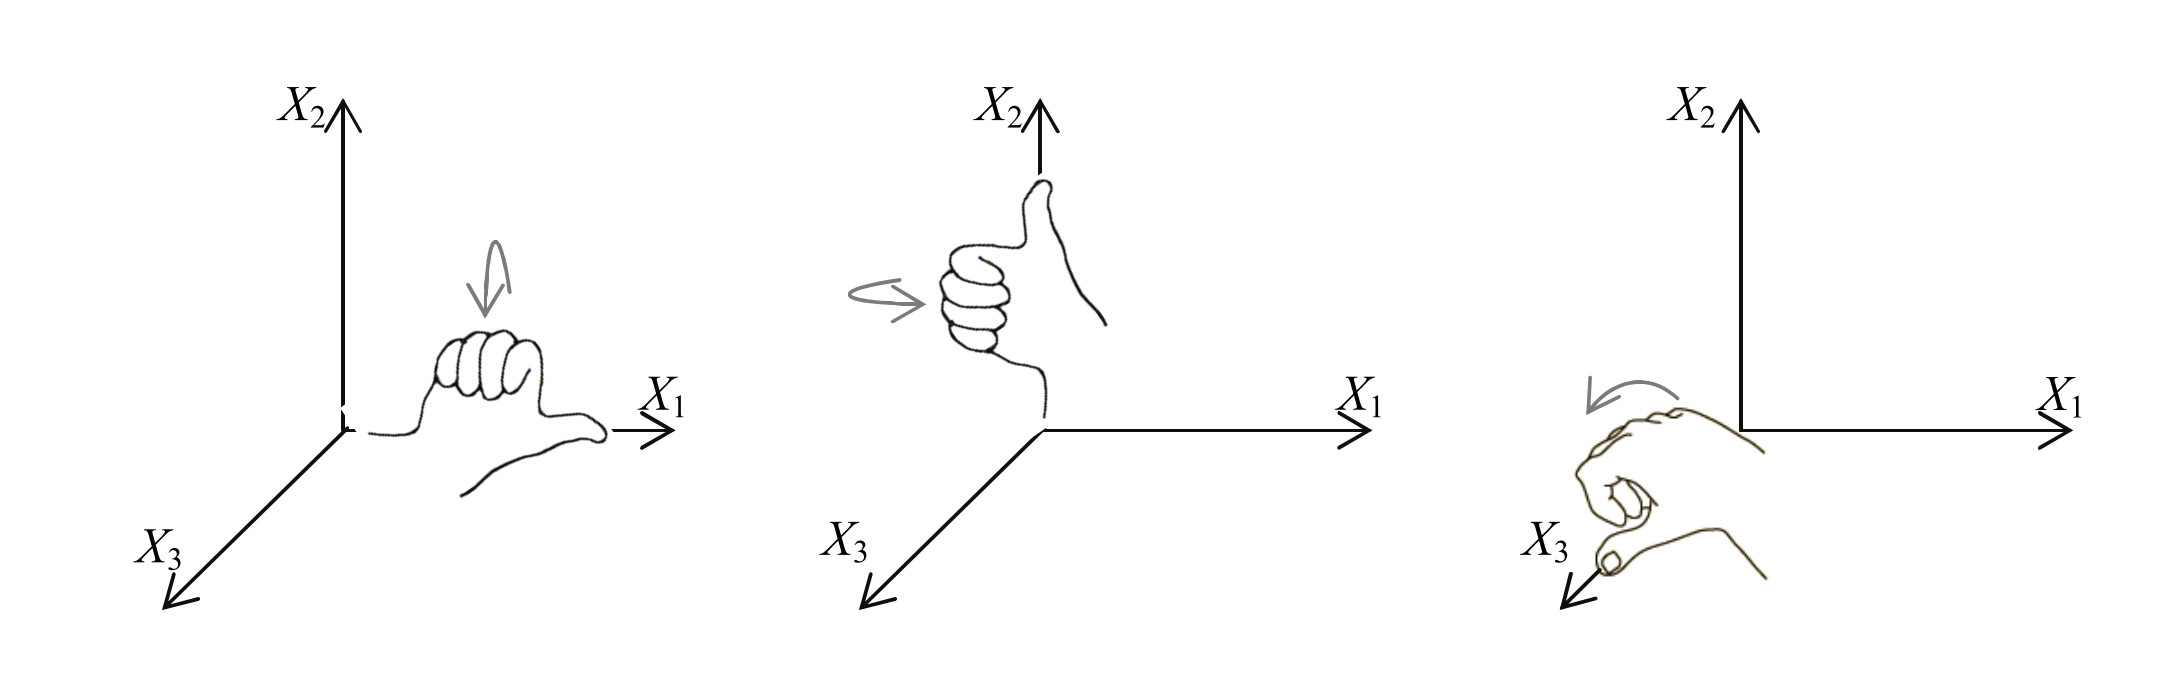
\includegraphics[width=14cm]{Img/GEO/geo-mano.jpg}
\centering
\end{figure}
\begin{center}
\textbf{\footnotesize{Regla de la mano derecha para obtener la dirección de un giro positivo en 3D.}}
\end{center}


Para entender el concepto de rotación en 3D como una extensión de la rotación 2D, hay que recordar que la rotación 2D es el giro sobre el eje de rotación, que es perpendicular al plano $X_{1}X_{2}$, el cual en 3D corresponde al eje $X_{3}$, entonces se obtiene la primera de las rotaciones principales.
De esta forma, por cada punto
$p = (x_{1},\ x_{2}^,\ x_{3})$ dado un ángulo $\theta$, puede ser rotado sobre el eje X3 en sentido contrario a las agujas del reloj, obteniendo las coordenadas del nuevo punto $p^{\prime} = (x_{1}^{\prime},\ x_{2}^{\prime},\ x_{3}^{\prime})$ de la misma forma en como se analizó en el espacio 2D quedando la coordenada x3 sin cambio, entonces, se extienden las formulas para la rotación 2D a 3D como: 

$$
\begin{cases}
{x_{1}}^{\prime} = x_{1} \cos(\theta) -x_{2} \sin(\theta) \\ 
{x_{2}}^{\prime} = x_{1} \sin(\theta) +x_{2} \cos(\theta) \\
{x_{3}}^{\prime} = x_{3}
\end{cases}
$$

\begin{center}
\textbf{Ecuación 3.11 \footnotesize{Fórmulas para la rotación 3D alrededor del eje $X_{3}$.}}
\end{center}

Sea $R_{3}(\theta)$ la matriz de rotación alrededor del eje $X_{3}$, en coordenadas homogéneas la rotación de un punto $p$ alrededor de dicho eje, se puede expresar como el producto matricial
$p^{\prime} = p.R_{3}(\theta)$, es decir:



$$
\begin{array}{rccl}
\left[
\begin{array}{rccl}
{x_{1}}^{\prime} & {x_{2}}^{\prime} & {x_{3}}^{\prime} & 1\\
\end{array}
\right]
\end{array}
=
\begin{array}{rccl}
\left[
\begin{array}{rccl}
x_{1} & x_{2} & x_{3} & 1\\
\end{array}
\right]
\end{array} 
.
\left[
\begin{array}{rccl}
\cos\theta & \sin\theta & 0 & 0\\
-\sin\theta & \cos\theta & 0 & 0\\
0 & 0 & 1 & 0\\
0 & 0 & 0 & 1\\
\end{array}
\right]
$$

\begin{center}
\textbf{\footnotesize{Expresión matricial para la rotación 3D alrededor del eje $X_{3}$}}
\end{center}

\begin{figure}[h]
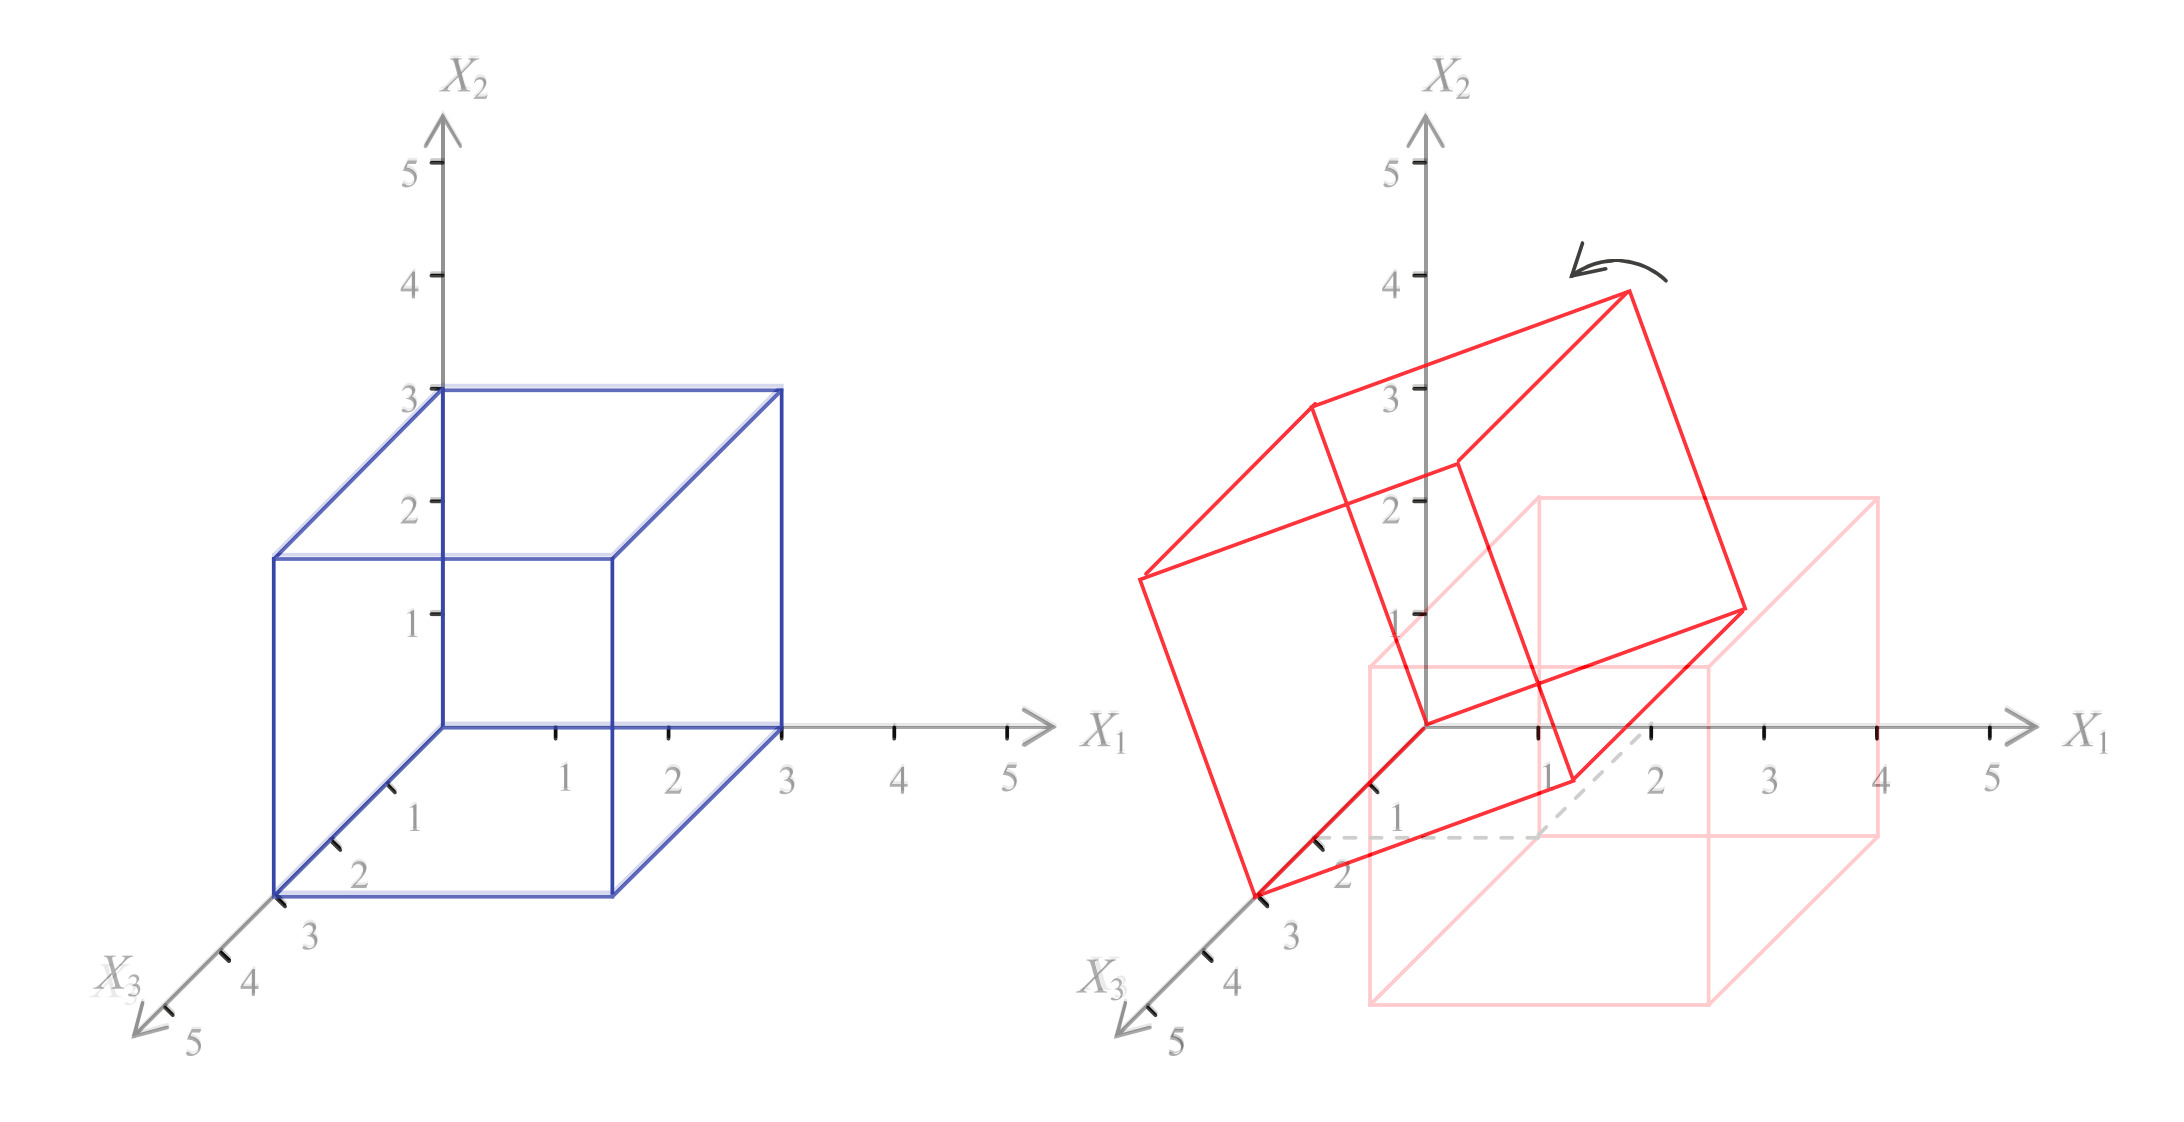
\includegraphics[width=12cm]{Img/GEO/geo-rotacion3d.jpg}
\centering
\end{figure}
\begin{center}
\textbf{\footnotesize{Ejemplo de rotación sobre el eje $X_{3}$ de una figura con $\theta = 20^{\circ}$}}
\end{center}

Las ecuaciones para las rotaciones sobre el eje $X_{1}$, y eje $X_{2}$, pueden ser obtenidas mediante las permutaciones cíclicas de los parámetros $X_{1}$, $X_{2}$, $X_{3}$: \vskip
\begin{center}
$X_{1}$\xrightarrow{}$X_{2}$\xrightarrow{}$X_{3}$
\end{center}

\begin{figure}[h]
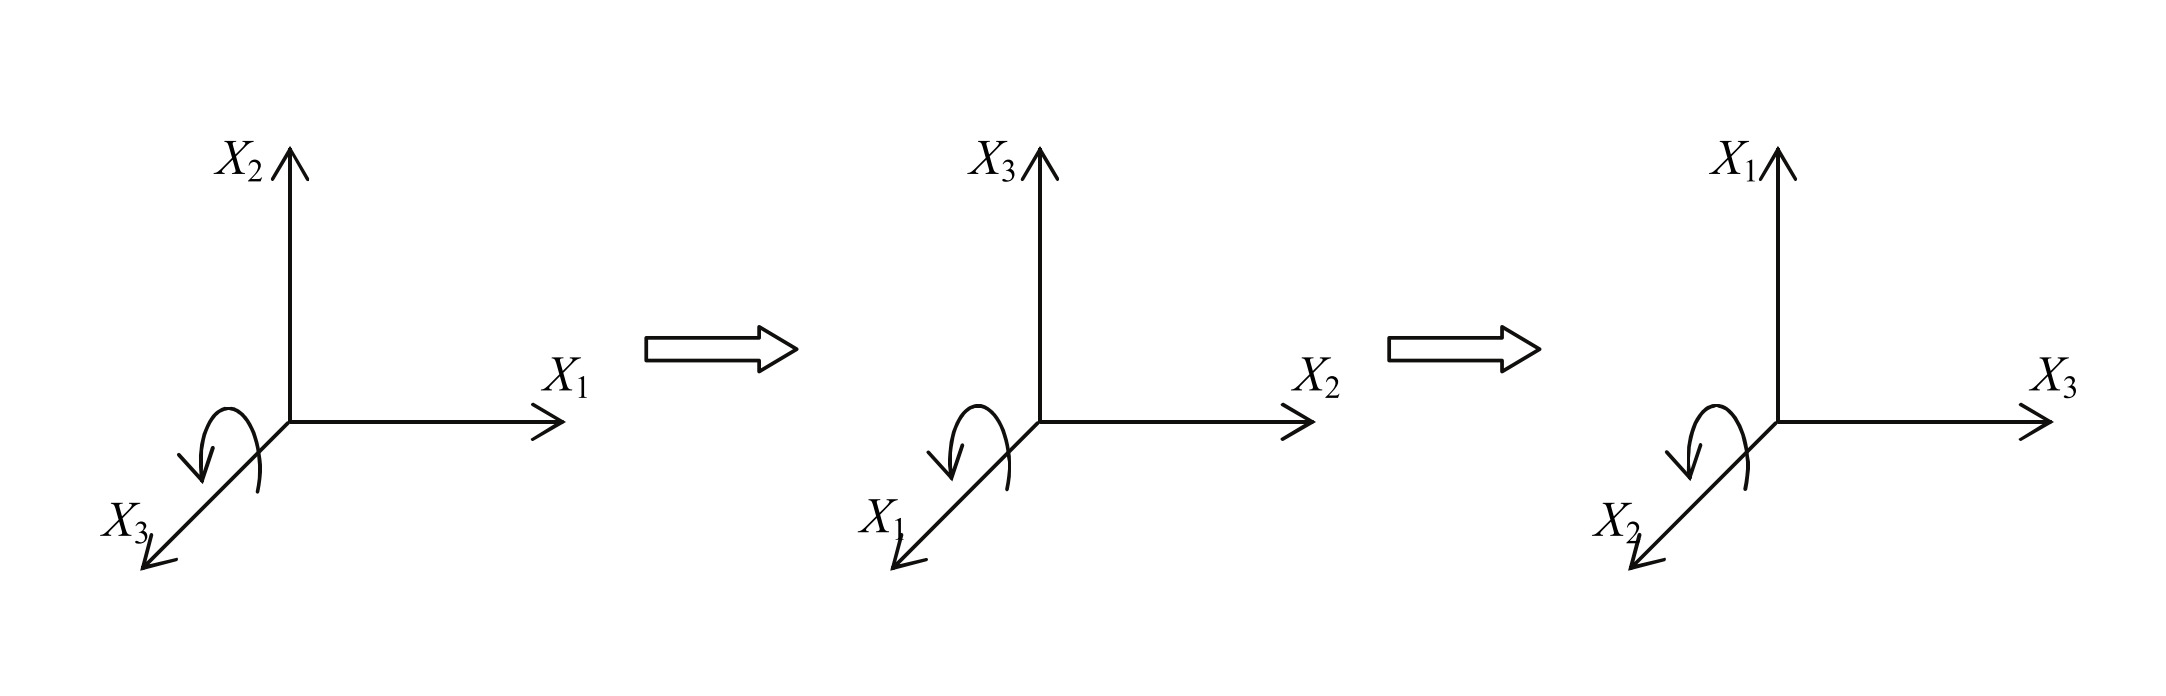
\includegraphics[width=12cm]{Img/GEO/geo-trans.jpg}
\centering
    \caption{\footnotesize{Permutaciones cíclicas de los ejes coordenados}}
\end{figure}

Entonces, aplicando estas substituciones cíclicas en la Ecuación 3.11, se obtienen las ecuaciones para la rotación alrededor del eje $X_{1}$ dado un ángulo
$\theta$


\begin{eqfloat}
\begin{equation*}
  \begin{split}
   \begin{cases}
{x_{2}}^{\prime} = x_{2} \cos(\theta) -x_{3} \sin(\theta) \\ 
{x_{3}}^{\prime} = x_{2} \sin(\theta) +x_{3} \cos(\theta) \\
{x_{1}}^{\prime} = x_{1}
\end{cases}
  \end{split}
\quad\longrightarrow\quad
  \begin{split}
   \begin{cases}
{x_{1}}^{\prime} = x_{1} \\ 
{x_{2}}^{\prime} = x_{2} \cos(\theta) -x_{3} \sin(\theta) \\
{x_{3}}^{\prime} = x_{2} \sin(\theta) +x_{3} \cos(\theta)
\end{cases}
\end{split}
\end{equation*}
\end{eqfloat}

\begin{center}
\textbf{\footnotesize{Fórmulas para la rotación 3D alrededor del eje X1. $X_{1}$}}
\end{center}
    
Sea $R_{1}( \theta )$ la matriz de rotación alrededor del eje $X_{1}$, en coordenadas homogéneas la
rotación de un punto p alrededor de dicho eje, se puede expresar como el producto matricial $p^{\prime} = p.R_{1}(\theta)$, es decir:

$$
\begin{array}{rccl}
\left[
\begin{array}{rccl}
{x_{1}}^{\prime} & {x_{2}}^{\prime} & {x_{3}}^{\prime} & 1\\
\end{array}
\right]
\end{array}
=
\begin{array}{rccl}
\left[
\begin{array}{rccl}
x_{1} & x_{2} & x_{3} & 1\\
\end{array}
\right]
\end{array} 
.
\left[
\begin{array}{rccl}
1 & 0 & 1 & 0\\
0 & \cos\theta & \sin\theta &  0\\
0 & -\sin\theta & \cos\theta & 0 \\
0 & 0 & 0 & 1\\
\end{array}
\right]
$$

\begin{center}
\textbf{\footnotesize{Expresión matricial para la rotación 3D alrededor del eje $X_{1}$}}
\end{center}

Aplicando nuevamente las substituciones cíclicas en la Ecuación 3.13, se obtienen las fórmulas para la rotación alrededor del eje $X_{2}$ dado un ángulo $\theta$

\begin{eqfloat}
\begin{equation*}
  \begin{split}
   \begin{cases}
{x_{3}}^{\prime} = x_{3} \cos(\theta) -x_{1} \sin(\theta) \\ 
{x_{1}}^{\prime} = x_{3} \sin(\theta) +x_{1} \cos(\theta) \\
{x_{2}}^{\prime} = x_{2}
\end{cases}
  \end{split}
\quad\longrightarrow\quad
  \begin{split}
   \begin{cases}
   {x_{1}}^{\prime} = x_{1} \cos(\theta) -x_{3} \sin(\theta) \\
   {x_{2}}^{\prime} = x_{2} \\ 
   {x_{3}}^{\prime} = x_{1} \sin(\theta) +x_{3} \cos(\theta)
\end{cases}
\end{split}
\end{equation*}
\end{eqfloat}

\begin{center}
\textbf{\footnotesize{Fórmulas para la rotación 3D alrededor del eje $X_{2}$}}
\end{center}

Sea $R_{2}( \theta )$ la matriz de rotación alrededor del eje $X_{2}$, en coordenadas homogéneas la
rotación de un punto p alrededor de dicho eje, se puede expresar como el producto matricial $p^{\prime} = p.R_{2}(\theta)$, es decir:

$$
\begin{array}{rccl}
\left[
\begin{array}{rccl}
{x_{1}}^{\prime} & {x_{2}}^{\prime} & {x_{3}}^{\prime} & 1\\
\end{array}
\right]
\end{array}
=
\begin{array}{rccl}
\left[
\begin{array}{rccl}
x_{1} & x_{2} & x_{3} & 1\\
\end{array}
\right]
\end{array} 
.
\left[
\begin{array}{rccl}
1 & 0 & 1 & 0\\
0 & \cos\theta & \sin\theta &  0\\
0 & -\sin\theta & \cos\theta & 0 \\
0 & 0 & 0 & 1\\
\end{array}
\right]
$$

\begin{center}
\textbf{\footnotesize{Expresión matricial para la rotación 3D alrededor del eje $X_{2}$}}
\end{center}

\subsubsection{Rotaciones 3D Como Rotaciones Paralelas a un Plano}

Las rotaciones en el espacio 3D son bien conocidas y entendidas por la mayoría de la
gente, y muchos pueden interpretarla como la rotación de un objeto alrededor de un eje (uni-dimensional) de rotación, sin embargo, es más adecuado pensar en un conjunto de rotaciones paralelas a un plano 2D, inmerso en el espacio. Se sabe que en 3D hay tres ejes coordenados: $X_1$, $X_2$ y $X_3$, y los planos principales son los formados por todas las posibles combinaciones de 2 de estos ejes, se obtienen así, los planos principales 3D: $X_1X_2$, $X_1X_3$ y $X_2X_3$.\vskip
Como vimos anteriormente, hay tres rotaciones principales, alrededor de cada uno los ejes principales, y durante estos giros se cumple que: dado el origen y ángulo de rotación, el conjunto de todos los puntos rotados por una matriz dada caen en un plano, llamado \textit{plano de rotación}, y el eje lineal de rotación es el que coincide con el vector normal de este plano. Esto es consistente con el espacio 2D, porque todos los puntos rotados caen en un único y mismo plano, el plano $X_1X_2$. \vskip
Entonces se tiene que las rotaciones alrededor de los ejes coordenados producen rotaciones de todos los planos paralelos al plano de rotación, el cuál está formado por los ejes restantes, es decir, si el eje de rotación es el eje $X_3$, el plano de rotación será el formado por los ejes coordenados restantes: el plano $X_1X_2$, de esta manera, si el eje de rotación es el eje $X_2$, el plano de rotación será el plano $X_1X_3$, y si el eje de rotación es el eje $X_1$, y el plano de rotación será el plano $X_2X_3$ (Figura 3.11 a) b) y c) respectivamente).

\begin{figure}[h]
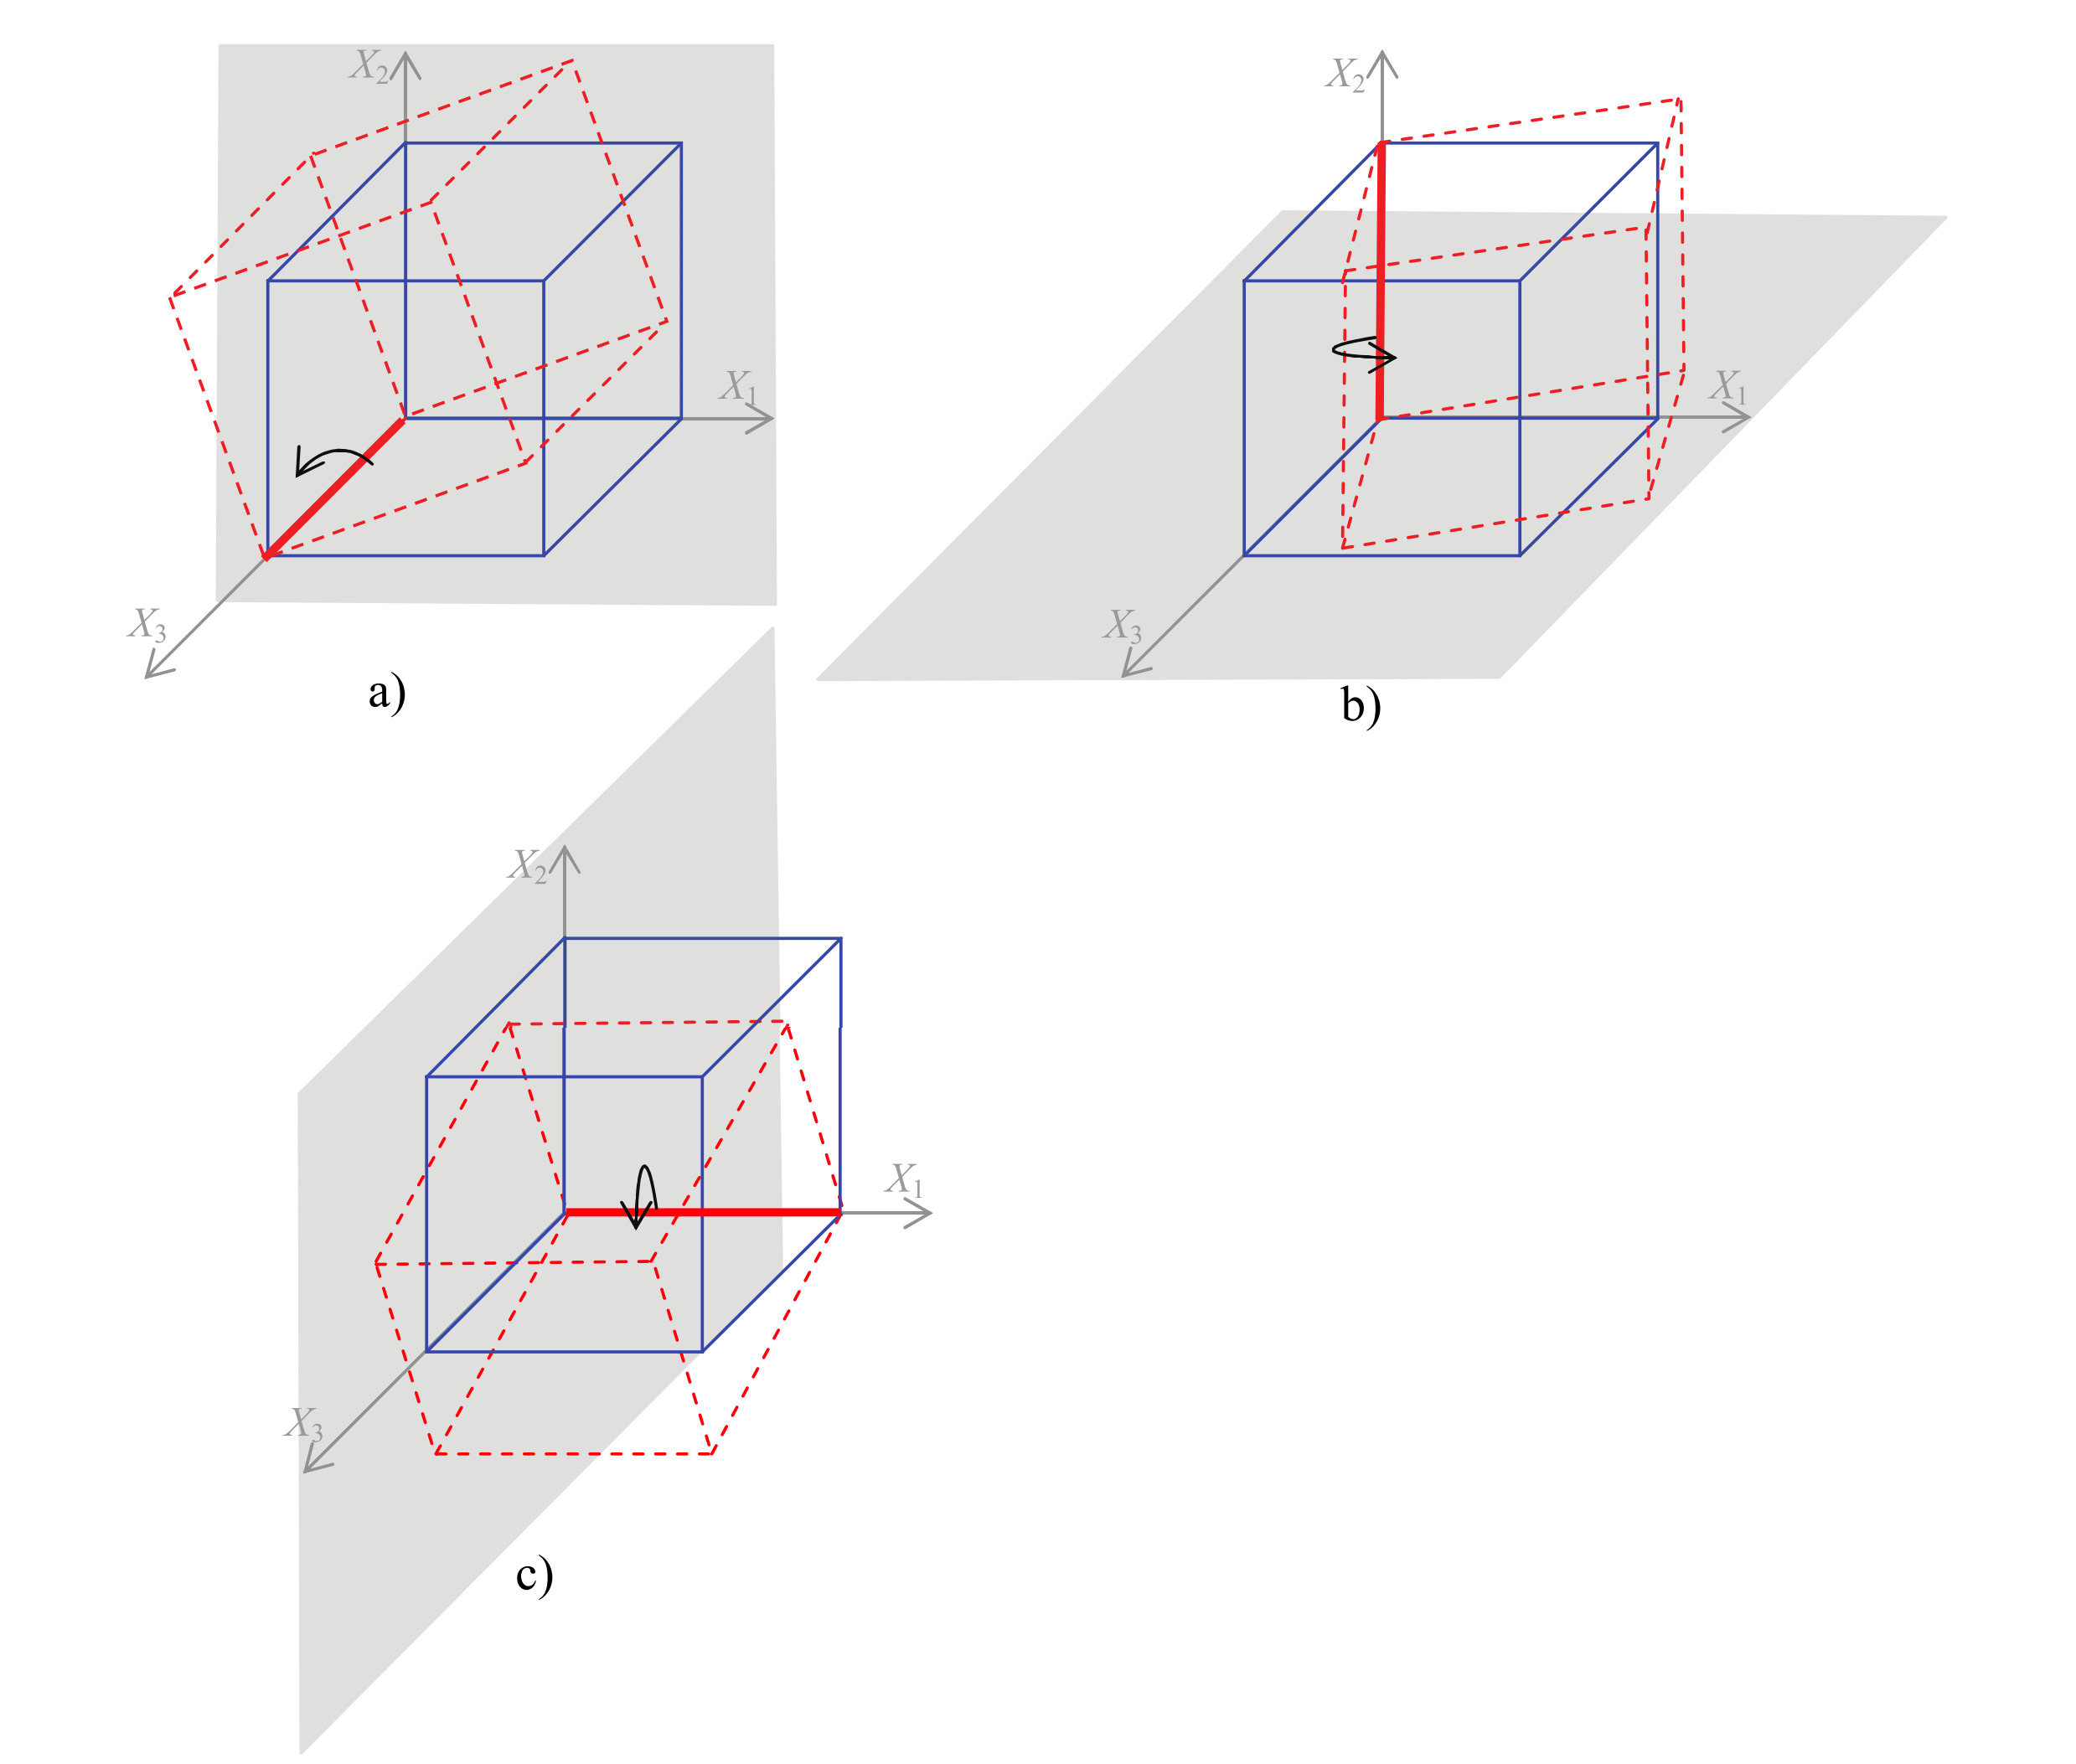
\includegraphics[width=14cm]{Img/GEO/geo-ejes.jpg}
\centering
\end{figure}

\begin{center}
\textbf{Figura 3.11. \footnotesize{Rotaciones principales 3D: a) eje $X_3$, plano $X_1X_2$,   b) eje $X_2$, plano $X_1X_3$   y c) eje $X_1$, plano $X_2X_3$.}}
\end{center}

También se cumple que las rotaciones 3D dejan fijo un subespacio uni-dimensional, tal subespacio es el eje de rotación, lo que significa que todos los puntos que caen sobre este eje, no se ven afectados por la rotación. Esto se puede ver gráficamente en la Figura 3.11, donde se observa que en cada una de las rotaciones, los puntos que caen sobre el eje de rotación no se ven afectados durante el giro. Si se renombran las matrices de rotación 3D, en términos de planos de rotación, colocando como subíndices los ejes que forman dicho plano, se tiene:

\begin{equation*}
   \begin{cases}
   \begin{array}{rccl}
    $$R_3(\theta) = R_{1,2}(\theta)
    =
    \left[
    \begin{array}{rccl}
    \cos\theta & \sin\theta & 0 & 0\\
    -\sin\theta & \cos\theta & 0  &  0\\
    0 & 0 & 1 & 0 \\
    0 & 0 & 0 & 1\\
    \end{array}
    \right]
    $$
    &
    $$R_1(\theta) = R_{2,3}(\theta)
    =
    \left[
    \begin{array}{rccl}
    1 & 0 & 1 & 0\\
    0 & \cos\theta & \sin\theta &  0\\
    0 & -\sin\theta & \cos\theta & 0 \\
    0 & 0 & 0 & 1\\
    \end{array}
    \right]
    $$\\ \\
    $$R_2(\theta) = R_{3,1}(\theta)
    =
    \left[
    \begin{array}{rccl}
    \cos\theta & 0 & -\sin\theta & 0\\
    0 & 1 & 0 &  0\\
    \sin\theta & 0 & \cos\theta & 0 \\
    0 & 0 & 0 & 1\\
    \end{array}
    \right]
    $$
    \end{array}
\end{cases}
\end{equation*}


\begin{center}
\textbf{Ecuacion 3.17.  \footnotesize{Renombramiento de las matrices de rotación 3D en términos de planos de rotación.}}
\end{center}


Como acabamos de ver las Rotaciones principales 3D se cumple cuando el plano de rotación y el eje (n-2)-dimensional están formados por los ejes coordenados. Si bien existen también las \textit{Rotaciones Generales 3D} cuando el plano de rotación y el eje están definido por puntos arbitrarios y no mediante los ejes coordenados, \vskip
En este trabajo 

VER SI SE ACLARA O NO

\subsubsection{Transformaciones Compuestas}
Con la representación matricial se puede aplicar una secuencia de transformaciones, calculando simplemente la multiplicación matricial de cada una de las matrices de transformación. Dado que se está manejando una representación de la posición de un punto p como vector renglón, se puede aplicar una transformación compuesta a un punto $p$, multiplicando las matrices de izquierda a derecha, comenzando con el punto $p$.
Por ejemplo, si se desea aplicar una translación, seguida de un escalamiento a un punto $p$, la posición final del punto $p^{\prime}$ se calcula de la siguiente manera:

$$p^{\prime} = (p. T(d)).S(s)$$
o bien una traslación seguida de una rotación:
$$p^{\prime} = (p.T(d)).R_{a,b}(\theta)$$

Las matrices de transformaciones compuestas para el caso que sean del mismo tipo, se comportan de la siguiente manera:

\begin{itemize}
  \item Las traslaciones sucesivas son aditivas: $T(d_a).T(d_b) = T(d_a + d_b)$
  \item Los escalamientos sucesivos son multiplicativos: $S(s_a).S(s_b) = S(s_a . s_b)$
  \item Las rotaciones sucesivas son aditivas: $R_{a,b}(\theta).R_{a,b}(\omega) = R_{a,b}(\theta + \omega)$
\end{itemize}


\subsection{Evolución Histórica del Modelado Geométrico}

Las raíces del Modelado Geométrico se encuentran en los primeros sistemas gráficos, que fueron desarrollados al comienzo de la década de los 60 con propósitos CAM. Esto dio lugar a la revolución industrial de la maquinaria numéricamente controlada (NC).
El siguiente paso importante fue dado en el MIT, con el desarrollo de un compilador para un lenguaje de descripción gráfica en 1967. Paralelamen te, las principales multinacionales en los campos automovilísticos, aviación, etc. desarrollaron sus primeros sistemas gráficos de diseño.
A mediados de los 70 se produjeron avances significativos en el Modelado Geométrico. Las limitaciones iniciales que presentaban los primeros sistemas gráficos fueron superadas desarrollando nuevas técnicas, las cuales permitieron realizar lo que conocemos como superficies esculpidas (sculptured surfaces), las superficies paramétricas, de Bezier, etc.
Mientras tanto, se desarrollaron los primeros modeladores alámbricos (wireframe) y los esquemas poligonales, de los cuales hablaremos más tarde. Inicialmente estos sistemas fueron bidimensionales y trataban de implantar lo que se conoce como dibujo técnico para se realizado con el ordenador.
Finalmente surgieron los esquemas de Modelado de Sólidos (o Modelado Sólido), sobre los que se desarrolla a continuación.

IMAGEN DE WIREFRAME VS SOLIDO


\section{Modelado Sólido}
\textit{El \textbf{Modelado Sólido} es una rama relativamente reciente del Modelado Geométrico, que hace hincapié en la aplicabilidad general de los modelos, e insiste en crear solamente modelos ``completos" de los sólidos, es decir, modelos
que son adecuados para responder algorítmicamente a cualquier pregunta geométrica que se formule. } 

El objetivo de ``aplicabilidad general" diferencia los esquemas de Modelado
Sólido de otros esquemas de modelado geométricos, los cuales se utilizan
en casos especiales. Así, los modelos gráficos (graphical models) se utilizan
para describir el dibujo técnico de los objetos, por ejemplo en ingeniería.
Los modelos de superficie (surface models) dan información detallada sobre superficies, pero no siempre proporcionan la información suficiente para determinar todas las propiedades geométricas. 
\vskip\vskip

\textcolor{red}{De acuerdo con el principio de universalidad, se espera de los modelos sólidos que sean capaces de responder algorítmicamente a las preguntas geométricas típicas que aparecen en las aplicaciones de ingeniería. Estos son algunos
ejemplos de dichas preguntas:
¿Cuál es el aspecto del objeto? ¿Cuál es su peso, área, etc.? ¿Toca el objeto a otro
si se mueven? ¿Qué carga puede soportar? ¿Cómo puede fabricarse con los procesos de
manufacturación disponibles?
La respuesta a estas preguntas podría ser una imagen, un número o una constante booleana. De hecho, incluso podría ser otro modelo sólido,
como por ejemplo en la siguiente pregunta: ¿cuál es el efecto del proceso de fabricación aplicado a este objeto? Obviamente, es importante que un sistema
de Modelado Geométrico incluya la posibilidad de modelar no sólo objetos físicos, sino también los efectos de aplicar sobre ellos procesos físicos. El sistema de modelado también debería ser capaz de realizar iteraciones, realizando
operaciones sobre los resultados obtenidos al hacer operaciones similares
anteriormente. Es decir, las operaciones disponibles en el sistema de
modelado deben formar un sistema cerrado donde se garantice que todas las operaciones mantengan la corrección de los modelos generados en las operaciones anteriores.
}

\begin{figure}[h]
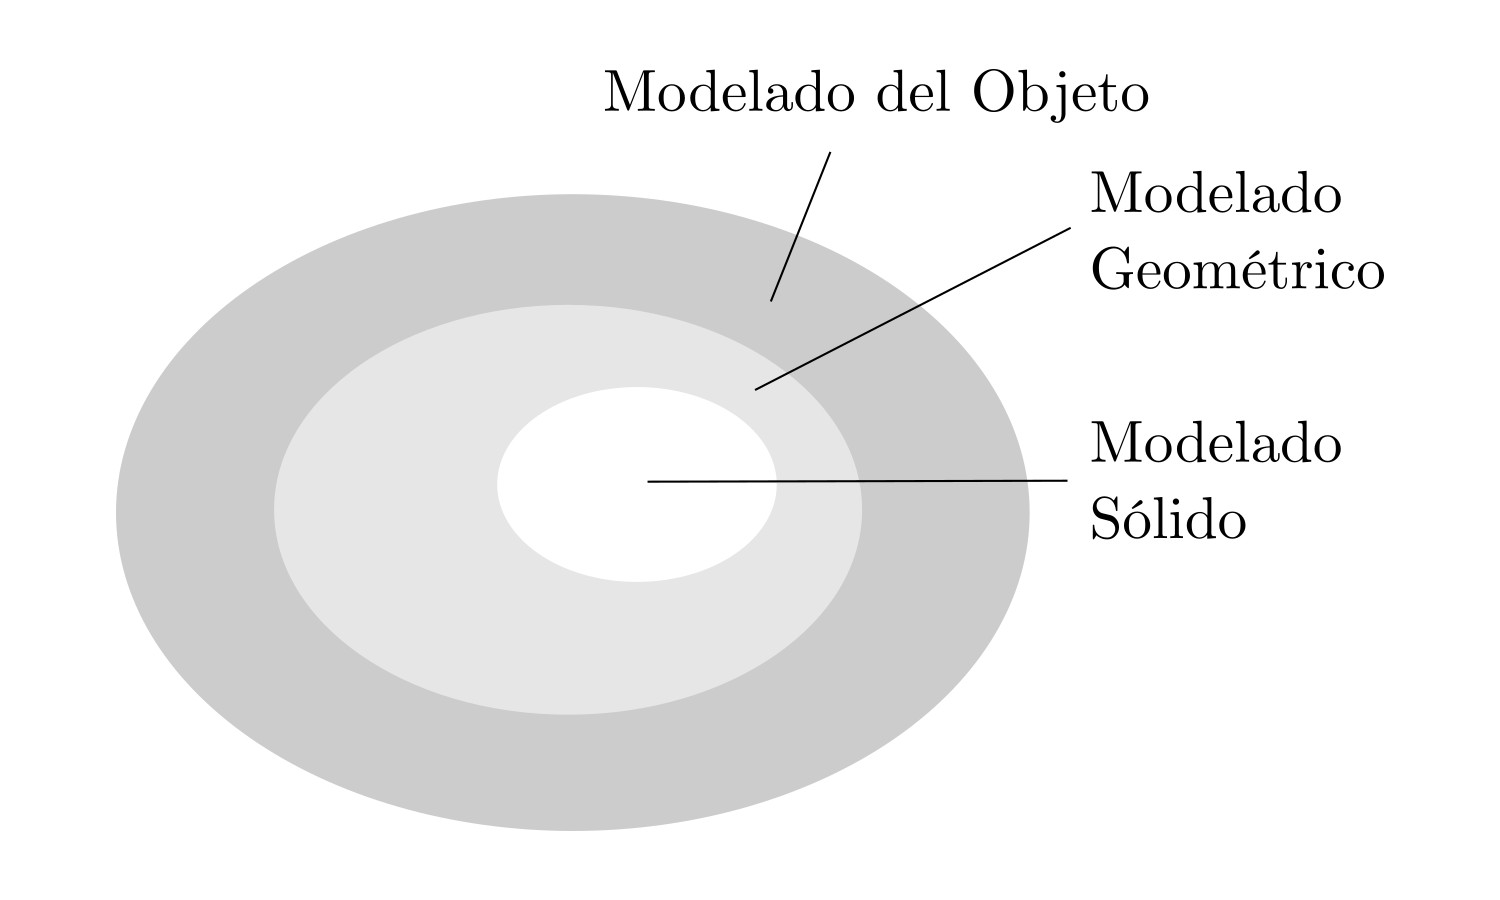
\includegraphics[width=10cm]{Img/GEO/geo-modelado0.jpg}
\centering
\end{figure}

\begin{center}
\textbf{Figura 3.11. \footnotesize{Estructura de subconjuntos en el Modelado.}}
\end{center}


\subsection{ Historia del Modelado Sólido }
Las universidades de Hokkaido y Cambridge desarrollaron los primeros sistemas
gráficos basados en esquemas de Modelado Sólido: TIPS y BUILD\cite{Toriya:1993:CPA:562297},
respectivamente. Se presentaron en Budapest en 1.973, demostrando su superioridad
sobre cualquier otro sistema de Modelado Geométrico.
TIPS utiliza figuras básicas o primitivas\footnote{ Las formas geométricas se consideradas primitivas por su básica constitución en las partes que la conforman por ejemplo cubo, cono, esfera.} y operaciones booleanas\footnote{Las operaciones booleanas se basan en los modelos que se estudian con el álgebra de Boole, se utilizan conceptos de suma, resta, intersección, etc. para el modelado de sólidos.} para definir sólidos en tres dimensiones. Esta técnica se conoce actualmente como Geometría Constructiva de Sólidos en inglés Constructive Solid Geometry (CSG), también llamado Modelado Booleano.
BUILD define los objetos como un conjunto de superficies, más la información
topológica que las relaciona (cómo se conectan las caras, aristas y vértices). Hoy se conoce esta técnica como la Representación por Fronteras en inglés Boundary Representation (B-Rep).
Desde entonces han surgido otros muchos modeladores, pero la gran
mayoría usan conceptos de los dos anteriores o incluso de ambos (Modeladores
Híbridos).
En 1977 se desarrolló en la universidad de Rochester (Estados Unidos)
el sistema gráfico PADL-1 \cite{Toriya:1993:CPA:562297}, que utiliza CSG para definir los objetos, pero que
puede convertir automáticamente las representaciones a B-Rep. La conversión
en sentido contrario presenta muchos problemas. 

IMAGEN EJEMPLO http://hopl.info/showlanguage.prx?exp=5287 

AGREGAR PROBLEMAS y LOS 2 METODOS b-surf y CSG

http://catarina.udlap.mx/u_dl_a/tales/documentos/msp/ruiz_r_r/capitulo2.pdf
http://di002.edv.uniovi.es/~rr/Tema7.pdf
http://di002.edv.uniovi.es/~rr/Tema8.pdf

\subsection{ Fundamentos del Modelado Sólido }
Un sistema de Modelado Sólido maneja dos tipos de información: los datos geométricos y datos topológicos. Los datos geométricos son aquellos que representan geométricamente los objetos (coordenadas de vértices, ecuaciones de superficies...). En cambio, los topológicos se refieren a cómo conectar componentes geométricos para conseguir un modelo.
A continuación se desarrollan las características topológicas más útiles en modelado (en 2 y 3D), que sirven principalmente para validar la integridad de los modelos.

\subsubsection{ Teorema del camino cerrado }
El giro total a lo largo de un camino cerrado es un entero múltiplo de 360°. Este entero se conoce como número de rotaciones (\textbf{Nr}) del camino. El valor de Nr es independiente de dónde se comience el recorrido del camino y de cómo esté orientado.

\begin{figure}[h]
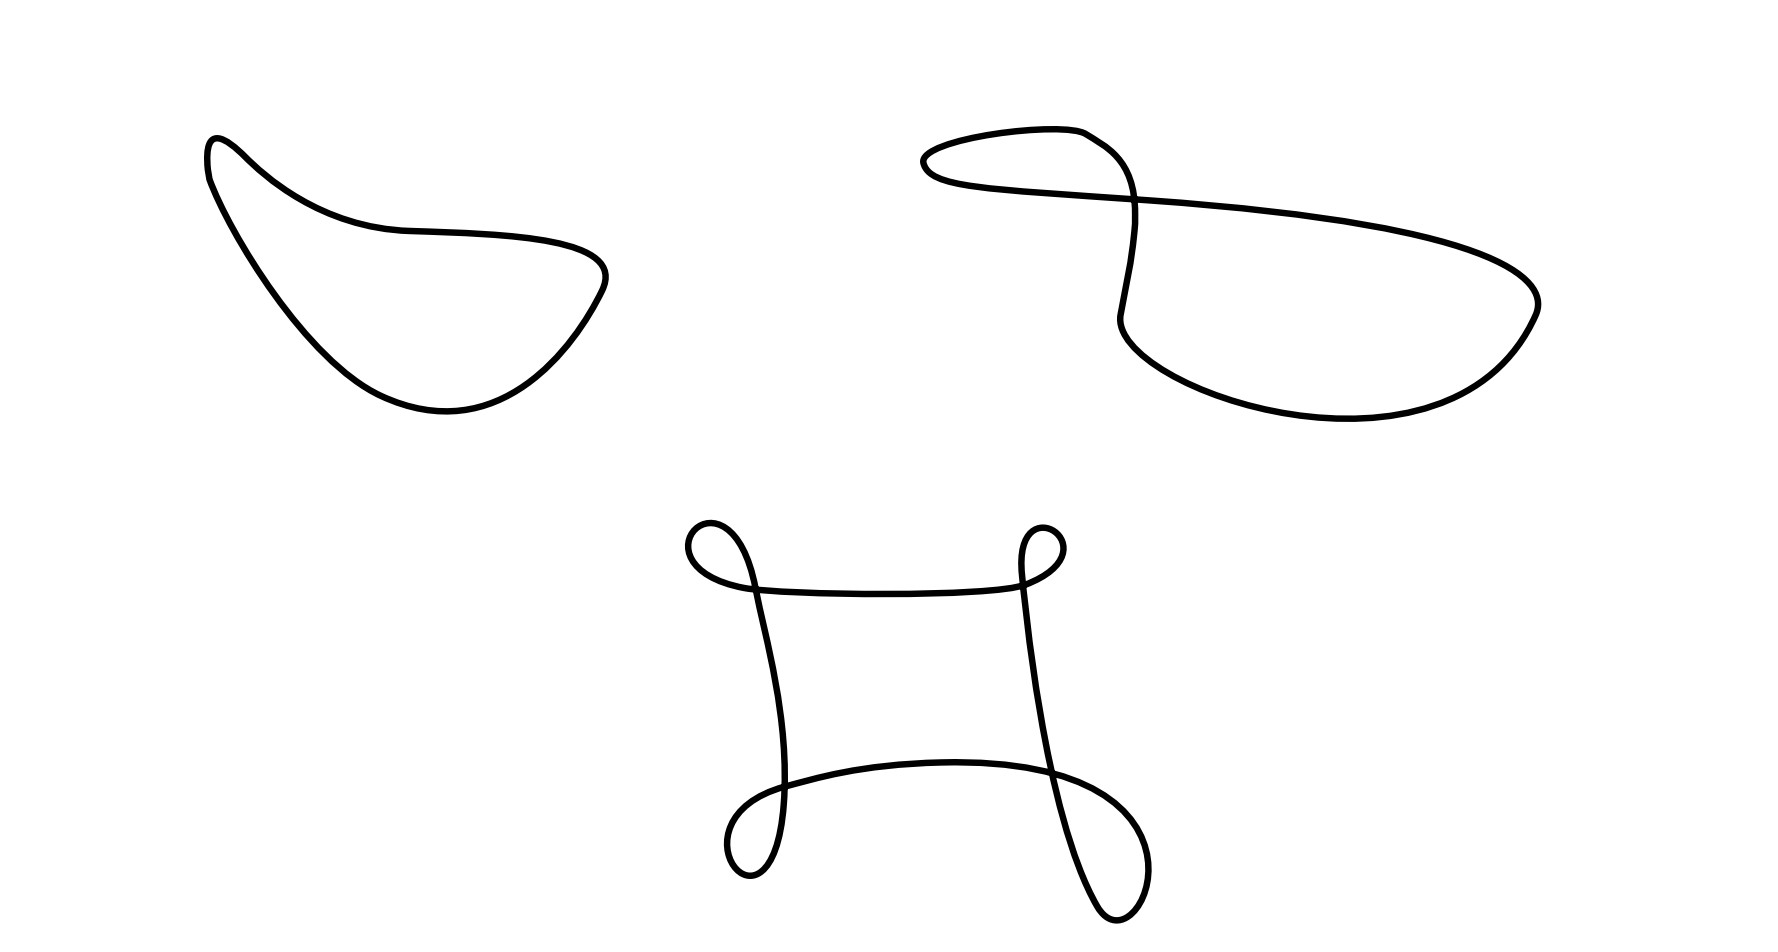
\includegraphics[width=8cm]{Img/GEO/geo-camino.jpg}
\centering
\end{figure}

\begin{center}
\textbf{Figura 3.11. \footnotesize{Ejemplo de caminos cerrados con valores de Nr diferentes.}}
\end{center}

\subsubsection{ Teorema del camino cerrado simple }
\textit{Un camino cerrado simple es aquél que no se corta a sí mismo}.\vskip
El teorema del camino cerrado simple dice que el giro total en un camino cerrado que no se corte a sí mismo es $\pm 360^\circ$. En otras palabras, el número de rotación Nr de un camino cerrado simple es $\pm1$.

\begin{figure}[h]
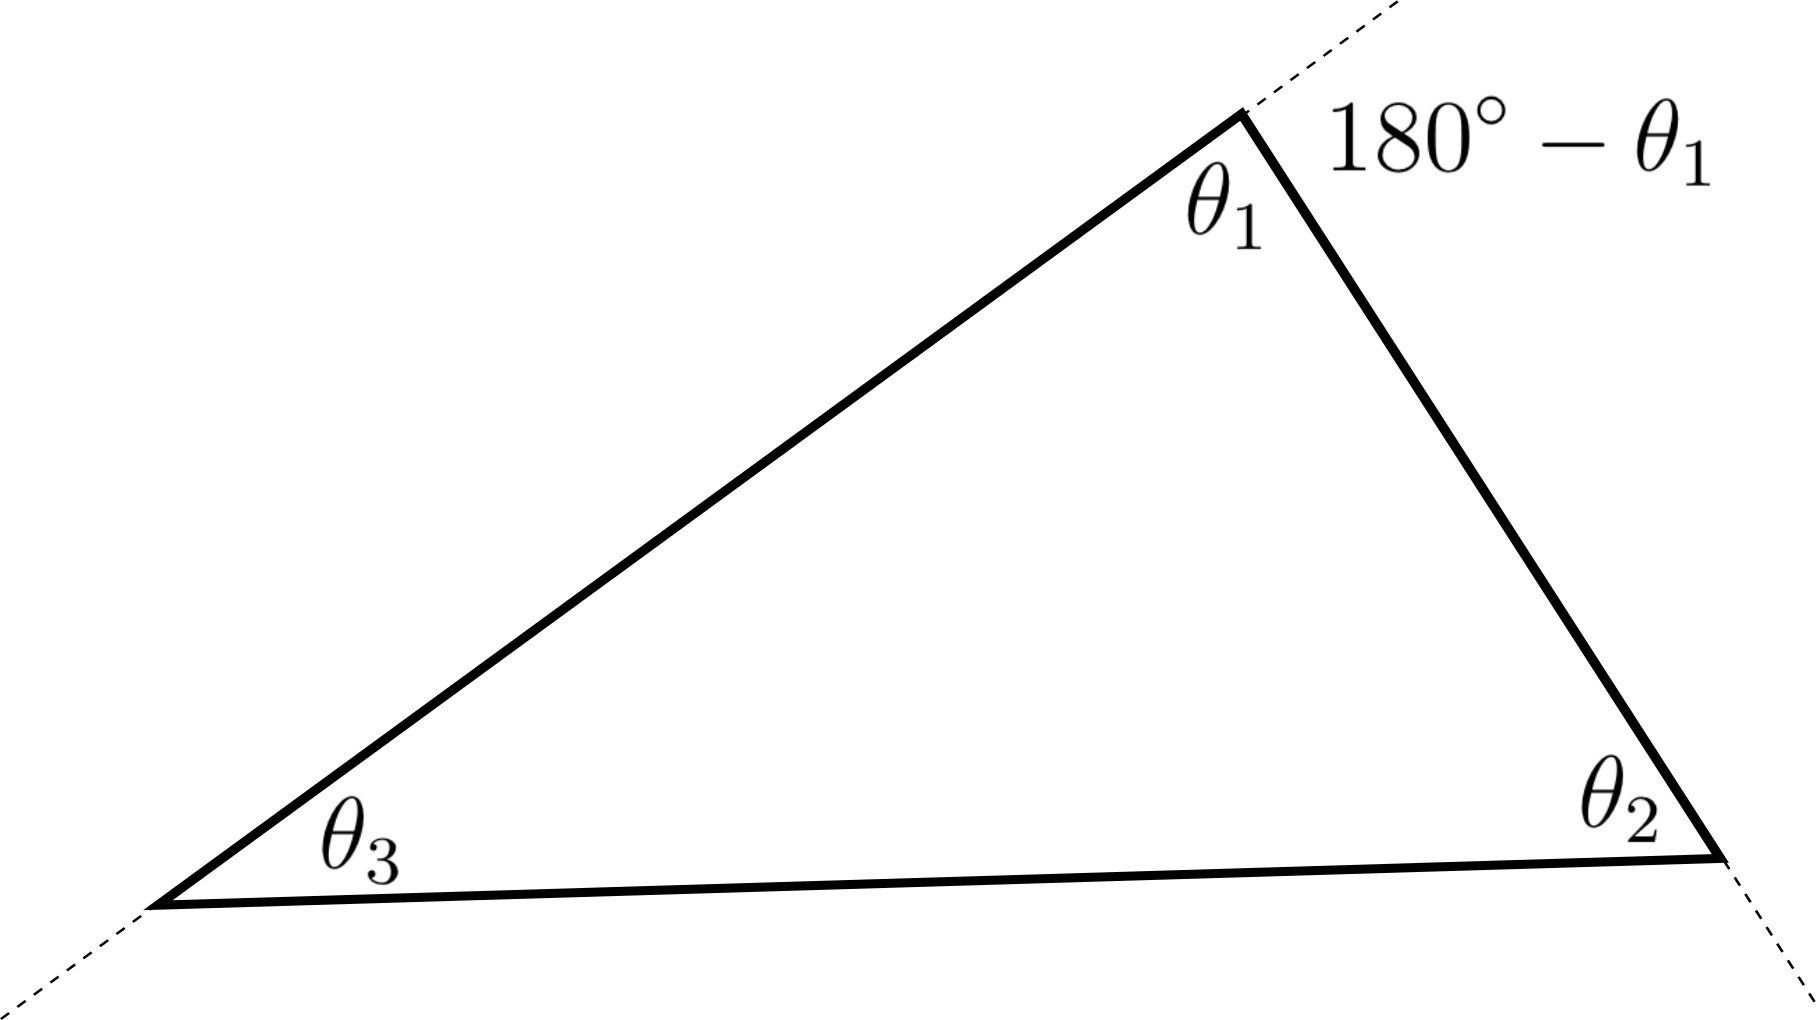
\includegraphics[width=8cm]{Img/GEO/geo-caminos.jpg}
\centering
\end{figure}

\begin{center}
\textbf{Figura 3.11. \footnotesize{La suma de los ángulos de giro en un camino cerrado simple es $\pm 360^\circ$}}
\end{center}

Por ejemplo, en el triángulo de la figura anterior, siendo $\theta_1, \theta_2$, y  $\theta_3$ sus ángulos internos, la suma de los ángulos de giro es:
$$(180^\circ - \theta_1) + (180^\circ - \theta_2 ) + (180^\circ - \theta_3) = 3\cdot180 - ( \theta_1 + \theta_2 + \theta_3) = 540 -180 = 360^\circ$$
Recordemos que la suma de los ángulos interiores de un triángulo (en la geometría euclidiana) es siempre $180^\circ$.\vskip
La importancia del teorema anterior en modelado radica en que es relativamente fácil medir los giros de los camino cerrados (ej., los ángulos de los polígonos), aplicando métodos locales. De este modo, si al finalizar el recorrido de un camino cerrado (aristas de un polígono) el acumulado final del giro es diferente a $360^\circ$ podemos asegurar que el modelo no es íntegro (está mal construido), ya que uno de sus polígonos se autointerseca, como ocurre en el ejemplo de la figura 3.9.

\begin{figure}[h]
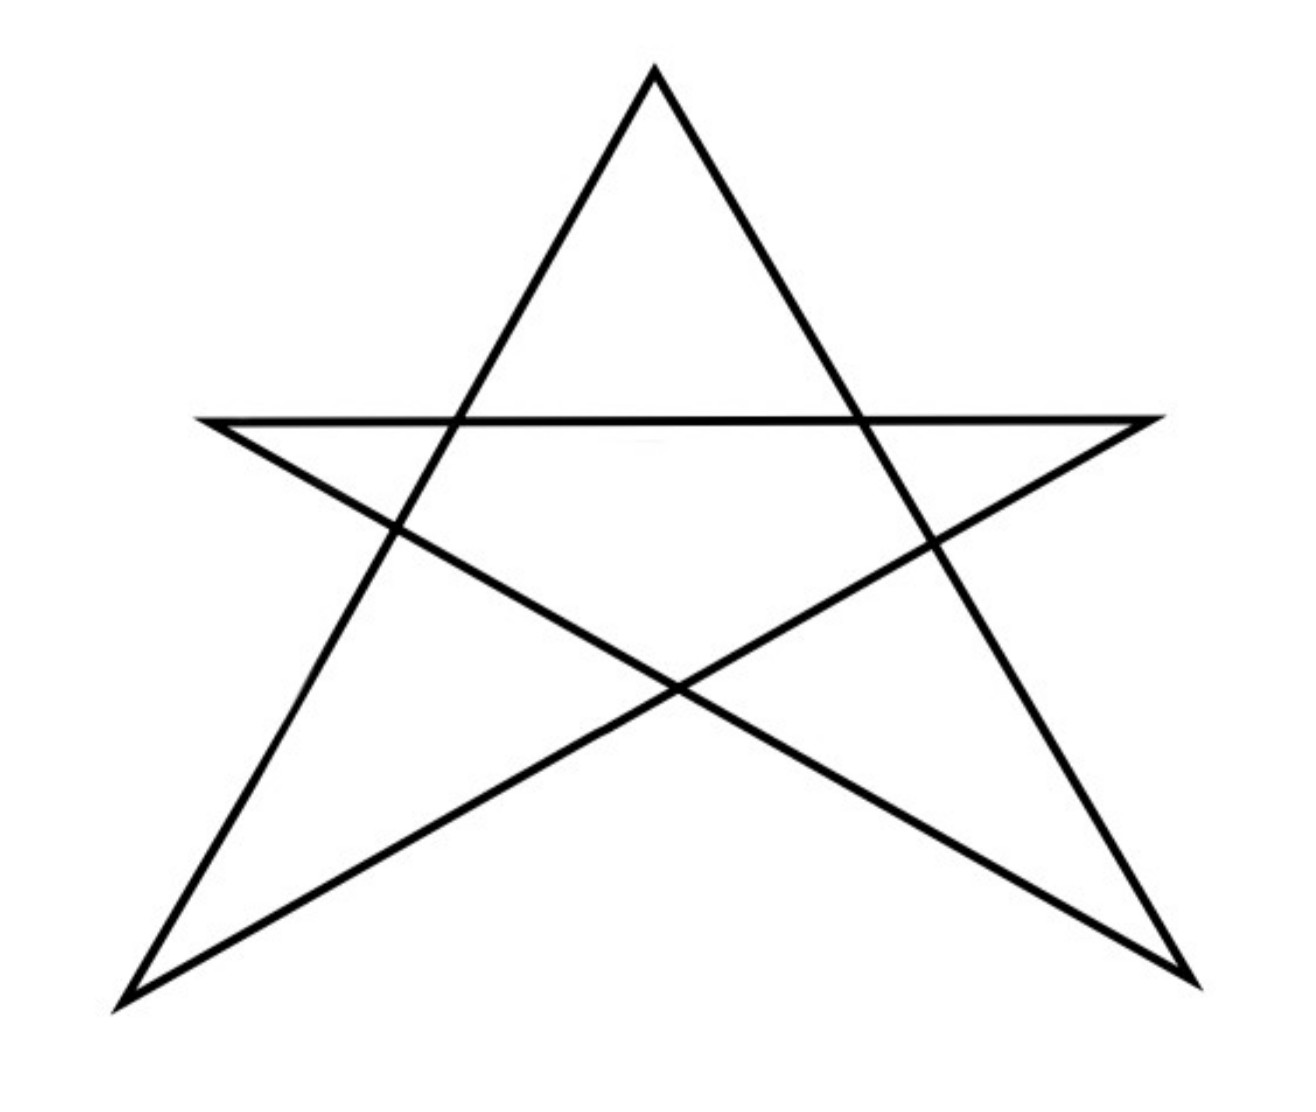
\includegraphics[width=6cm]{Img/GEO/geo-caminon.jpg}
\centering
\end{figure}

\begin{center}
\textbf{Figura 3.11. \footnotesize{La suma de los ángulos de giro en un camino cerrado no simple es diferente de $\pm 360^\circ$}}
\end{center}

\subsubsection{ Deformación de curvas y planos }

El teorema de deformación de curvas y planos dice que \textit{cualquier curva cerrada simple de un plano se puede transformar mediante una isotopía de ambiente en un cuadrado}.\vskip
En 1936, H.Whitney y W.C.Graustein observaron que dos caminos cerrados coplanarios pueden transformarse el uno en el otro sólo si tienen el mismo giro total. Este resultado junto con el teorema anterior se puede utilizar para probar el teorema del camino cerrado simple: por una parte, cualquier curva cerrada simple en un plano se puede transformar en un cuadrado, y además, un camino cerrado sólo puede transformarse en otro si tiene el mismo giro total. Entonces se puede deducir que cualquier camino cerrado simple tiene el mismo giro total que un cuadrado, es decir, $\pm 360^\circ$, con lo que se demuestra el teorema.\vskip
Las transformaciones pueden ser de dos tipos:

\begin{itemize}
\item \textit{Homotopía regular}. Es una deformación que produce cambios en el camino.
\item \textit{Isotopía de ambiente}. Supongamos que tenemos el camino dibujado sobre una lámina de goma. Si estiramos o encogemos la lámina por diferentes puntos,podemos conseguir que varíe la trayectoria del camino, o sea, una isotopía de ambiente o transformación de hoja de goma.
\end{itemize}

La homotopía regular es más violenta (no conservadora) que la isotopía de ambiente (conservadora), ya que puede crear o eliminar puntos de corte, cosa que no hace esta última. De hecho, una isotopía de ambiente es un caso especial de la homotopía regular, en la que no se añaden ni eliminan puntos de corte.

\begin{figure}[h]
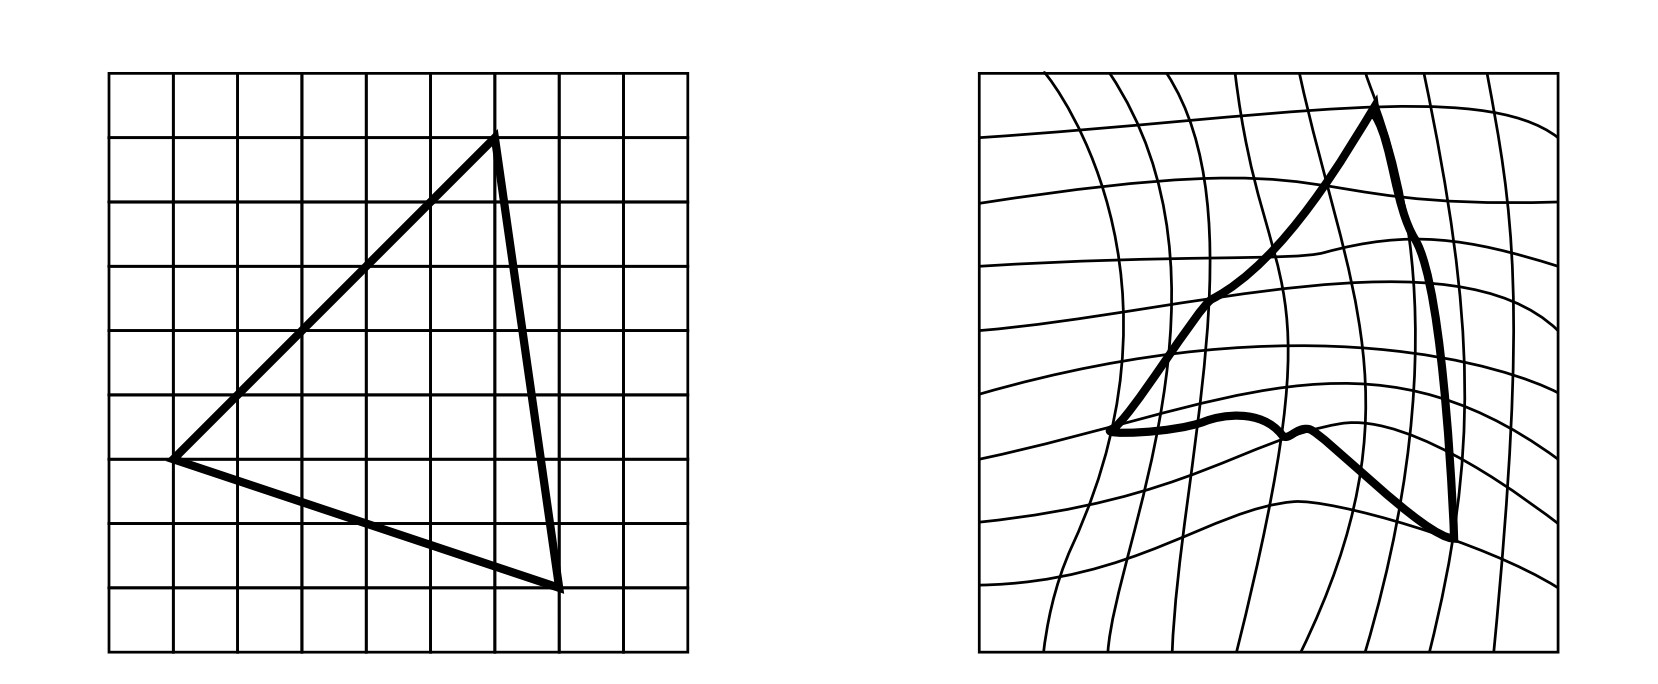
\includegraphics[width=12cm]{Img/GEO/geo-goma.jpg}
\centering
\end{figure}

\begin{center}
\textbf{Figura 3.11. \footnotesize{Deformación conservadora en una hoja de goma}}
\end{center}

\subsubsection{ Teorema de la curva de Jordan }
Se deduce del teorema de deformación de curvas y planos y dice que \textit{cualquier curva cerrada simple en un plano, divide a éste en dos regiones: una interior y otra exterior.} Da igual de qué curva cerrada simple se trate, pues siempre va a dividir al plano en una
parte interior a la curva y otra exterior. Este teorema es válido sólo para curvas que estén en superficies planas, ya que podemos trazar una curva cerrada simple en un toro, por ejemplo, y no dividirlo en dos regiones.
El interior de la curva es deformable mediante una isotopía de ambiente y puede
transformarse en un cuadrado. Una región, plana o no, que pueda ser transformada mediante una isotopía de ambiente en un cuadrado se llama \textit{disco topológico} y se caracteriza porque no tiene huecos ni puntos aislados en él.

\subsubsection{ Ángulo de Exceso }

Se conoce como ángulo de exceso (o simplemente exceso), \textit{el ángulo de giro implícito a un camino cerrado trazado sobre una superficie.} También se define como el giro que experimenta un puntero de referencia cuando es llevado alrededor de un camino cerrado. Como pronto se verá, el ángulo de exceso está íntimamente relacionado con la curvatura de las superficies.\vskip
El concepto de ángulo de exceso sirve para generalizar el teorema del camino cerrado simple, de modo que también sea válido para caminos cerrados simples sobre superficies
curvas. La generalización de este teorema nos dice que el giro total a lo largo de un camino cerrado simple, más el ángulo de exceso, debe ser igual a $360^\circ$, es decir, que:
$$T+E=360$$
donde:

\begin{description}
\item T = Giro Total a lo largo del camino.
\item E = Ángulo de exceso a lo largo del camino.
\end{description}

Para aclarar este concepto obsérvese la figura siguiente

\begin{figure}[h]
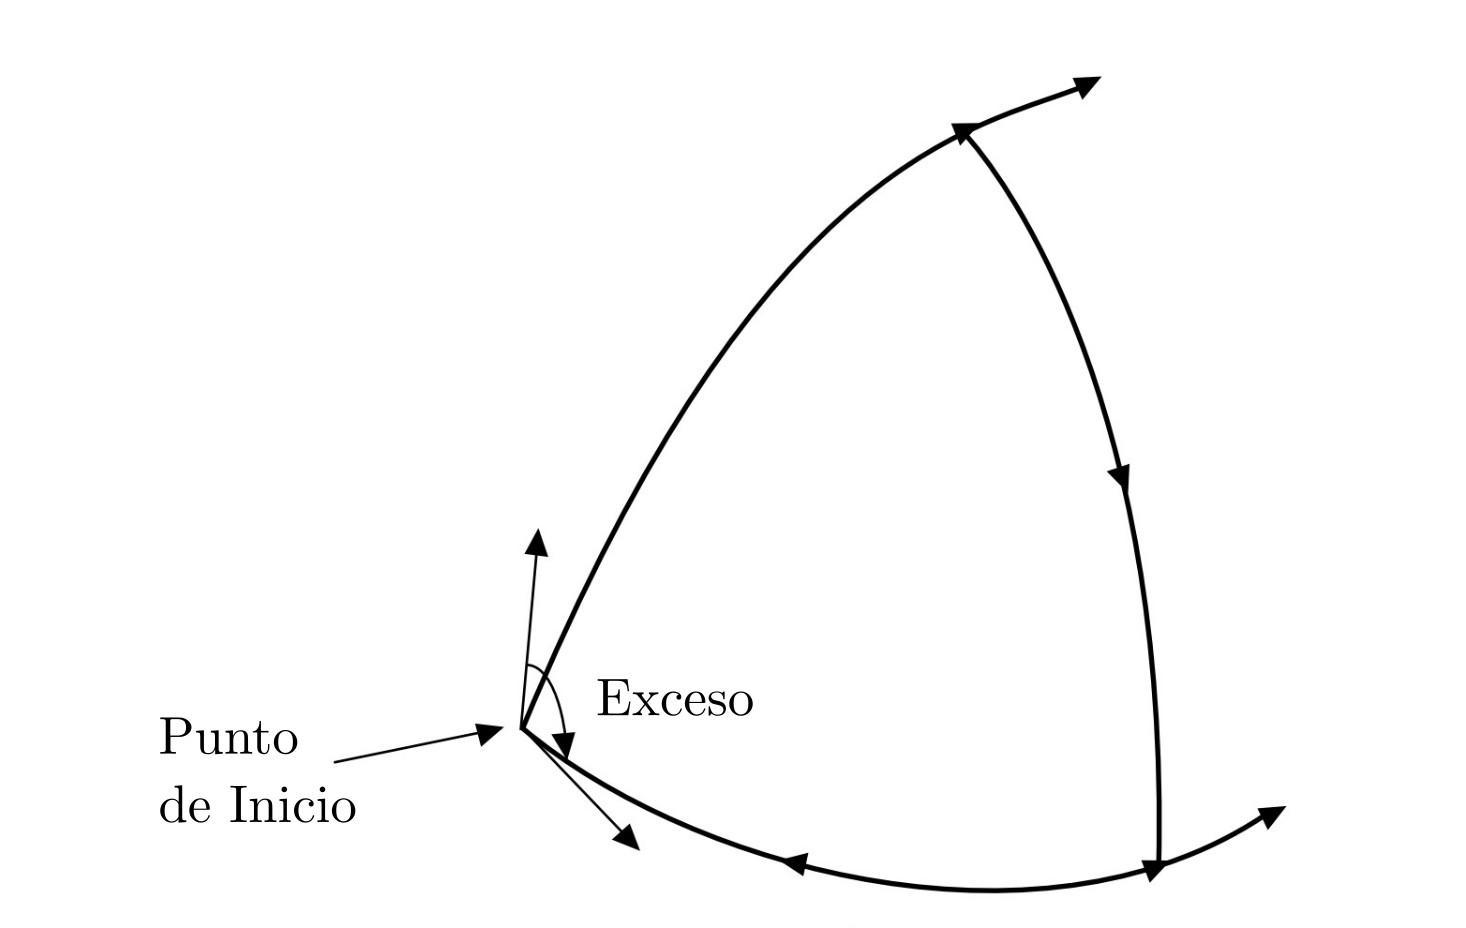
\includegraphics[width=12cm]{Img/GEO/geo-curva.jpg}
\centering
\caption{\textbf{Figura 3.11. \footnotesize{Concepto de ángulo de exceso}}}
\end{figure}

En esta figura se representa un cuadrante esférico. Supongamos que comenzamos a
andar desde el punto de inicio, con un puntero sobre nuestra cabeza apuntando hacia el polo. Al llegar a éste, giramos $90^\circ$ para volver al ecuador (obsérvese que sólo giramos nosotros, no el puntero, por lo que entre nuestra nariz y el puntero hay un ángulo de $90^\circ$).
De vuelta en el ecuador, damos otro giro de $90^\circ$ para regresar al punto de inicio (ahora
nuestra nariz y el puntero miran en direcciones opuestas). Una vez allí damos otro giro de $90^\circ$ que nos dejará en la posición inicial.
Se puede ver que el giro total que hemos realizado es de $90^\circ.3 = 270^\circ$ Luego $T = 270^\circ$. En cambio lo que ha girado el puntero (ángulo de exceso) es $E = 90^\circ$. Sumando ambas cantidades obtenemos $360^\circ$ que es lo que afirma el teorema.\vskip

\textit{Cuanto más curva es la superficie mayor es el ángulo de exceso. Si la superficie es plana, el ángulo de exceso es cero.}\vskip

\textbf{Propiedades del ángulo de exceso:} \vskip
a) Para un determinado camino, su ángulo de exceso es siempre el mismo, independientemente de donde comience el recorrido.\vskip
b) El ángulo de exceso es aditivo. Así, el exceso de cualquier polígono es igual a la suma de los excesos de los subpolígonos en que se subdivida.



\subsubsection{ Curvatura total de las superficies }

\textit{Para cualquier disco topológico en una superficie cualquiera, el exceso que se obtiene alrededor de su frontera es igual a la curvatura total del interior.}
Como el exceso posee la propiedad aditiva, si se subdivide una superficie cualquiera en piezas o trozos poligonales, y para cada polígono se calcula el ángulo de exceso, la suma de los excesos de cada polígono se conoce como \textit{curvatura total de la superficie}, y se representa por K.
\textit{La curvatura total es una constante topológica para todas las superficies cerradas}; por ejemplo, todas las esferas tienen la misma curvatura total.
Por tanto, se puede usar el ángulo de exceso para averiguar la curvatura total de un objeto, simplemente recorriendo caminos cerrados dibujados en la superficie y calculando sus ángulos de exceso.
\vskip

\textbf{Evaluación de la curvatura en los modelos 3D cerrados}\vskip
Dos superficies cerradas son \textbf{topológicamente equivalentes} si es posible transformar una superficie en otra mediante \textit{transformaciones conservativas}, es decir, deformaciones que no rompan o corten la superficie. Por ejemplo, un cubo y una esfera son topológicamente equivalentes, ya que es posible (al menos mentalmente) transformar progresivamente el cubo hasta convertirlo en una esfera, y viceversa. En cambio, el toro y la esfera no lo son, ya que no es posible obtener un toro a partir de una esfera sin romper (rasgar) la superficie de ésta.
\textit{Todos los objetos cerrados que son topológicamente equivalentes poseen la misma curvatura.}

\textbf{A) Esferas, toros y asas}

Se puede calcular la curvatura total de los objetos de diferentes familias topológicas, a partir de la curvatura total de estos tres tipos de objetos: esferas, toros y asas.
Según vimos, el exceso de un cuadrante esférico es de $90^\circ$, o lo que es igual, su curvatura es de $\pi/2$. Como todos los cuadrantes son iguales, la curvatura total de la semiesfera es $2\pi$; por tanto, la curvatura total de la esfera será de $4\phi$ $(K = 4\pi)$.
Por otro lado, aunque no se incluya la demostración, un toro (un donut o rosquilla) tiene una curvatura total 0 $(K = 0)$, lo que no implica que el toro sea plano, sino que tiene tanta curvatura positiva como negativa.\vskip
Un toro, topológicamente hablando, puede considerarse como una esfera con un asa.
El proceso de añadir asas a las esferas no es una deformación topológica conservativa, ya que se ha de cortar la superficie de éstas, para pegar las asas. Esto implica que el objeto original y el resultante (después de añadir las asas) no son topológicamente equivalentes.
Para construir un toro a partir de una esfera se procede como sigue: primero se achatan (aplanan) dos regiones circulares en la esfera. De cada región se recorta un disco liso. A continuación se pega (o cose) un asa en los huecos dejados por los discos; el asa es un cilindro hueco (tubo) y sus aristas deben hacerse coincidir con los bordes de los discos recortados. El resultado obtenido será un toro como se muestra en la figura 11.

\begin{figure}[h]
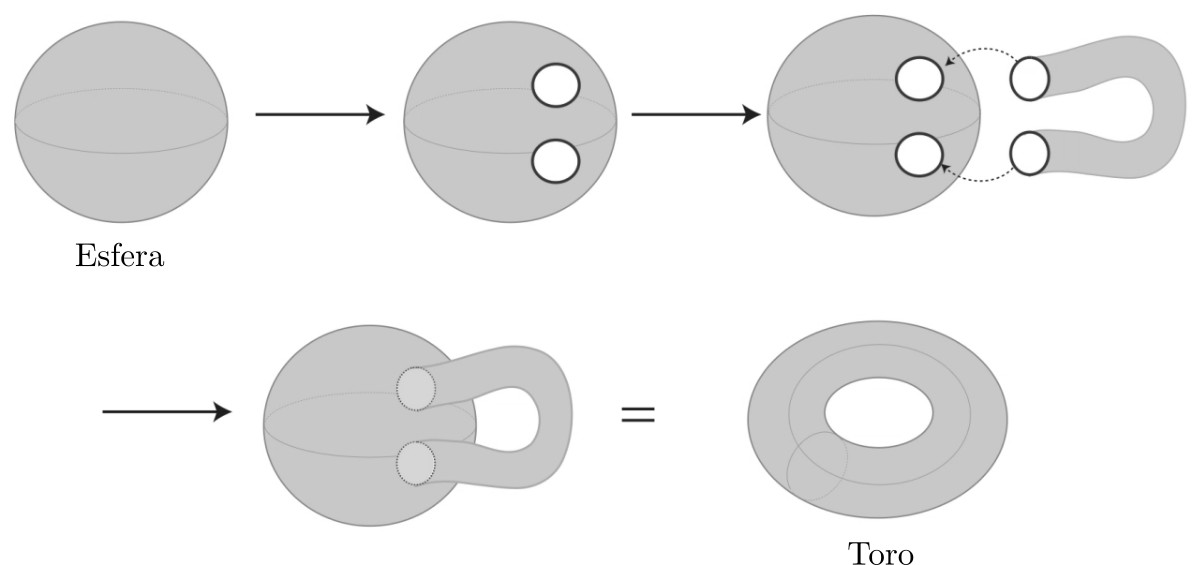
\includegraphics[width=15cm]{Img/GEO/geo-asa.jpg}
\centering
\caption{\textbf{Figura 3.11. \footnotesize{Construcción de un Toro a partir de una Esfera}}}
\end{figure}

En otras palabras:\vskip 
$$esfera - 2discos + asa = toro$$
Para calcular la curvatura total del asa, en la Ec. 3 se sustituyen los objetos por su curvatura correspondiente $(4\pi \ – \ 2\cdot0 + K_{asa} = 0)$ obteniéndose que la curvatura del asa es $–4\pi$. Por tanto, vemos que al añadir asas a cualquier superficie, la curvatura total de dicha superficie disminuye en $4\pi$. Además, observamos también que un toro con dos agujeros es topológicamente equivalente a un toro con un asa y a una esfera con dos asas.
En general, para una superficie topológicamente equivalente a una esfera con $g$ asas, la curvatura total es
$$K_{esfera \ con \ g  \ asas} = 4_{\pi}(1 - g)$$

\begin{figure}[h]
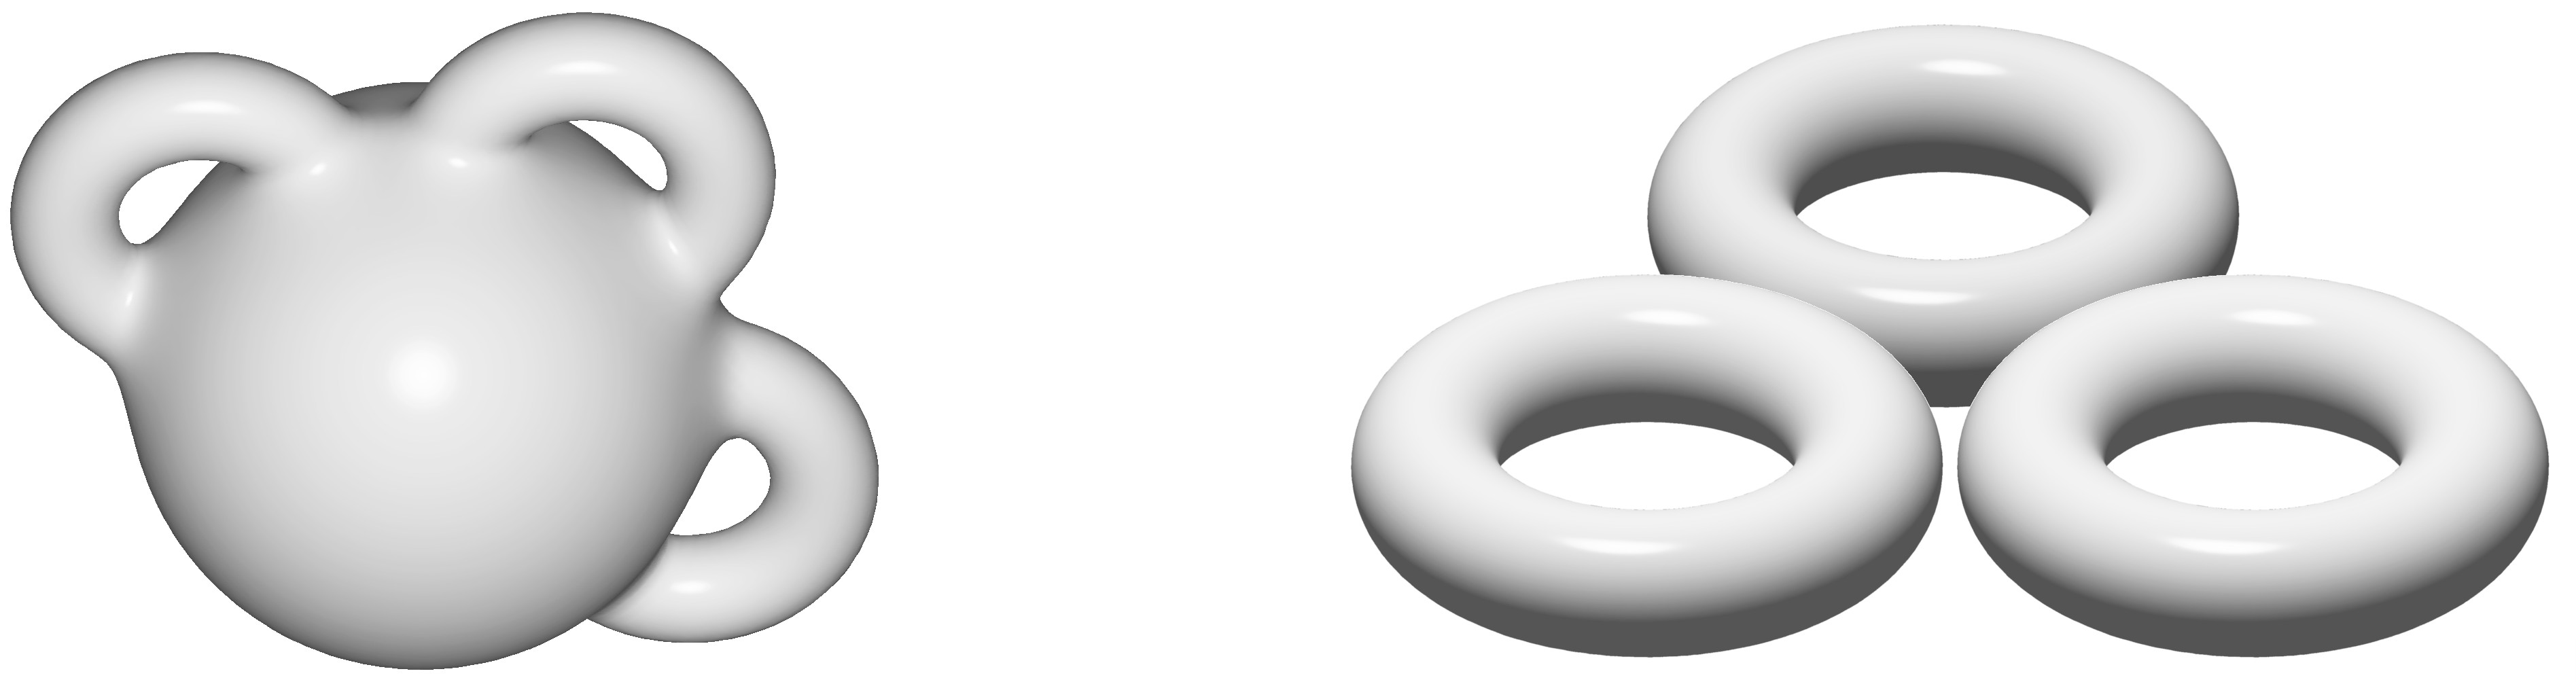
\includegraphics[width=14cm]{Img/GEO/geo-toro.jpg}
\centering
\caption{\textbf{Figura 3.11. \footnotesize{equivalente topológico a una esfera con tres asas}}}
\end{figure}

$``g”$ se conoce como \textit{orden o grado del objeto} y también como \textit{orden de la superficie}.
La importancia de esto es que cualquier superficie cerrada tridimensional que no se corte a si misma es topológicamente equivalente a una esfera con $g$ asas. Por ejemplo, una superficie como la mostrada en la figura 12
es topológicamente equivalente a una esfera con 3 asas.
De la Ec. 4 se deduce que \textit{la curvatura total de una superficie cerrada
en el espacio tridimensional es un múltiplo de $4\pi$}. Ver esta afirmación no
es otra cosa que la versión 3D del teorema del camino cerrado, o bien, del
teorema de camino cerrado simple si $g = 0$. Esta característica topológica de
las superficies cerradas es muy útil para la construcción y la validación de la
integridad de los modelos complicados, ya que normalmente se conoce la familia topológica $(g)$ del objeto modelado. Para ello se compara la curvatura
calculada con la indicada por la Ec. 4. Si se desconoce $g$, al menos es posible
verificar que su curvatura sea un múltiplo de $4\pi$.


\subsubsection{ Estudio de los modelos de caras planas o poliedros }

El estudio de los modelos de caras planas tiene una importancia especial debido a que muchos esquemas de representación usan poliedros y la topología asociada a los mismos.
Por poliedro (poli- muchos, edro- cara) entendemos una disposición de polígonos de forma que solamente dos polígonos se unen en una arista, formando el conjunto de polígonos una superficie cerrada. Además, es posible recorrer la superficie del poliedro siguiendo sus aristas.

\begin{figure}[h]
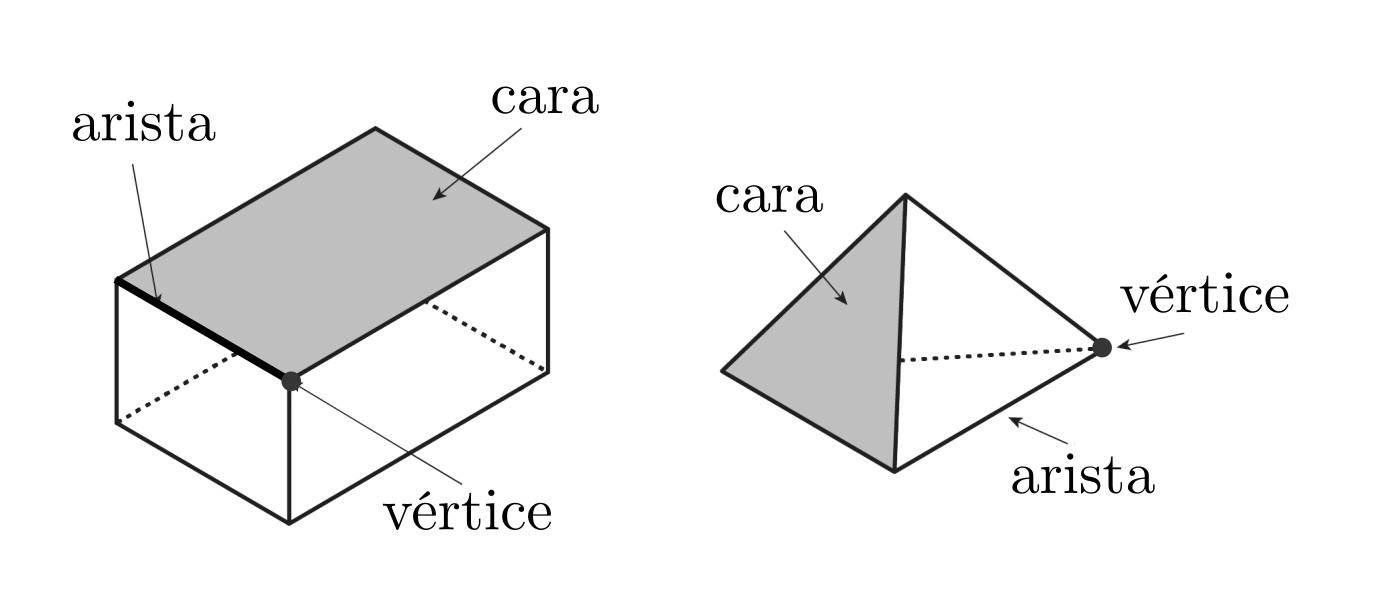
\includegraphics[width=12cm]{Img/GEO/geo-vertex.jpg}
\centering
\caption{\textbf{Figura 3.11. \footnotesize{Caras, aristas y vértices en 2 poliedros diferentes (prisma rectangular y tetraedro)}}}
\end{figure}


\textbf{Características topológicas de los poliedros}

Conocer las características topológicas de los poliedros es importante en la construcción de los modelos y especialmente para su validación. A continuación se ven los tipos de poliedros más importantes para el modelado y sus propiedades topológicas.

\textbf{A) Poliedros simples}\vskip
Un poliedro simple es aquél que puede ser transformado de forma continua en una esfera, o sea, que es topológicamente equivalente a una esfera $(g = 0)$\vskip
Los poliedros regulares forman un subconjunto de los poliedros simples, cuya característica principal es que todas sus caras (polígonos) son iguales.
\begin{description}
\item i. Fórmula de Euler para los poliedros simples.\vskip
Para un poliedro simple se cumple que el número de vértices, menos el número de aristas, más el número de caras es 2, es decir
$$V - A  +  C = 2$$
Según esta fórmula, se puede demostrar que sólo hay 5 poliedros regu- lares: tetraedro, hexaedro o cubo, octaedro, dodecaedro e icosaedro.
\item ii. Fórmula de Euler-Poincaré.\vskip
Poincaré generalizó la fórmula de Euler para el espacio n-dimensional. En lugar de puntos, aristas y caras, él definió elementos de $0, 1, ..., n-1$ dimen- siones. A cada uno de estos elementos lo llamó, $N_0, N_1,..., N_{n}-1$, respectiva- mente, y expresó la fórmula de Euler como
$$N_0 - N_1 + N_2 - ... = 1-(-1)^n$$ Para $n = 3$ se obtiene la fórmula de Euler. 
\end{description}


\textbf{B) Poliedros no simples. Número de conectividad y de orden}\vskip
Los \textit{poliedros no simples} son los equivalentes topológicos de cualquier objeto sólido con huecos, por lo que son muy útiles en el Modelado Sólido. En la figura 13 hay algunos ejemplos de poliedros no simples.

\begin{figure}[h]
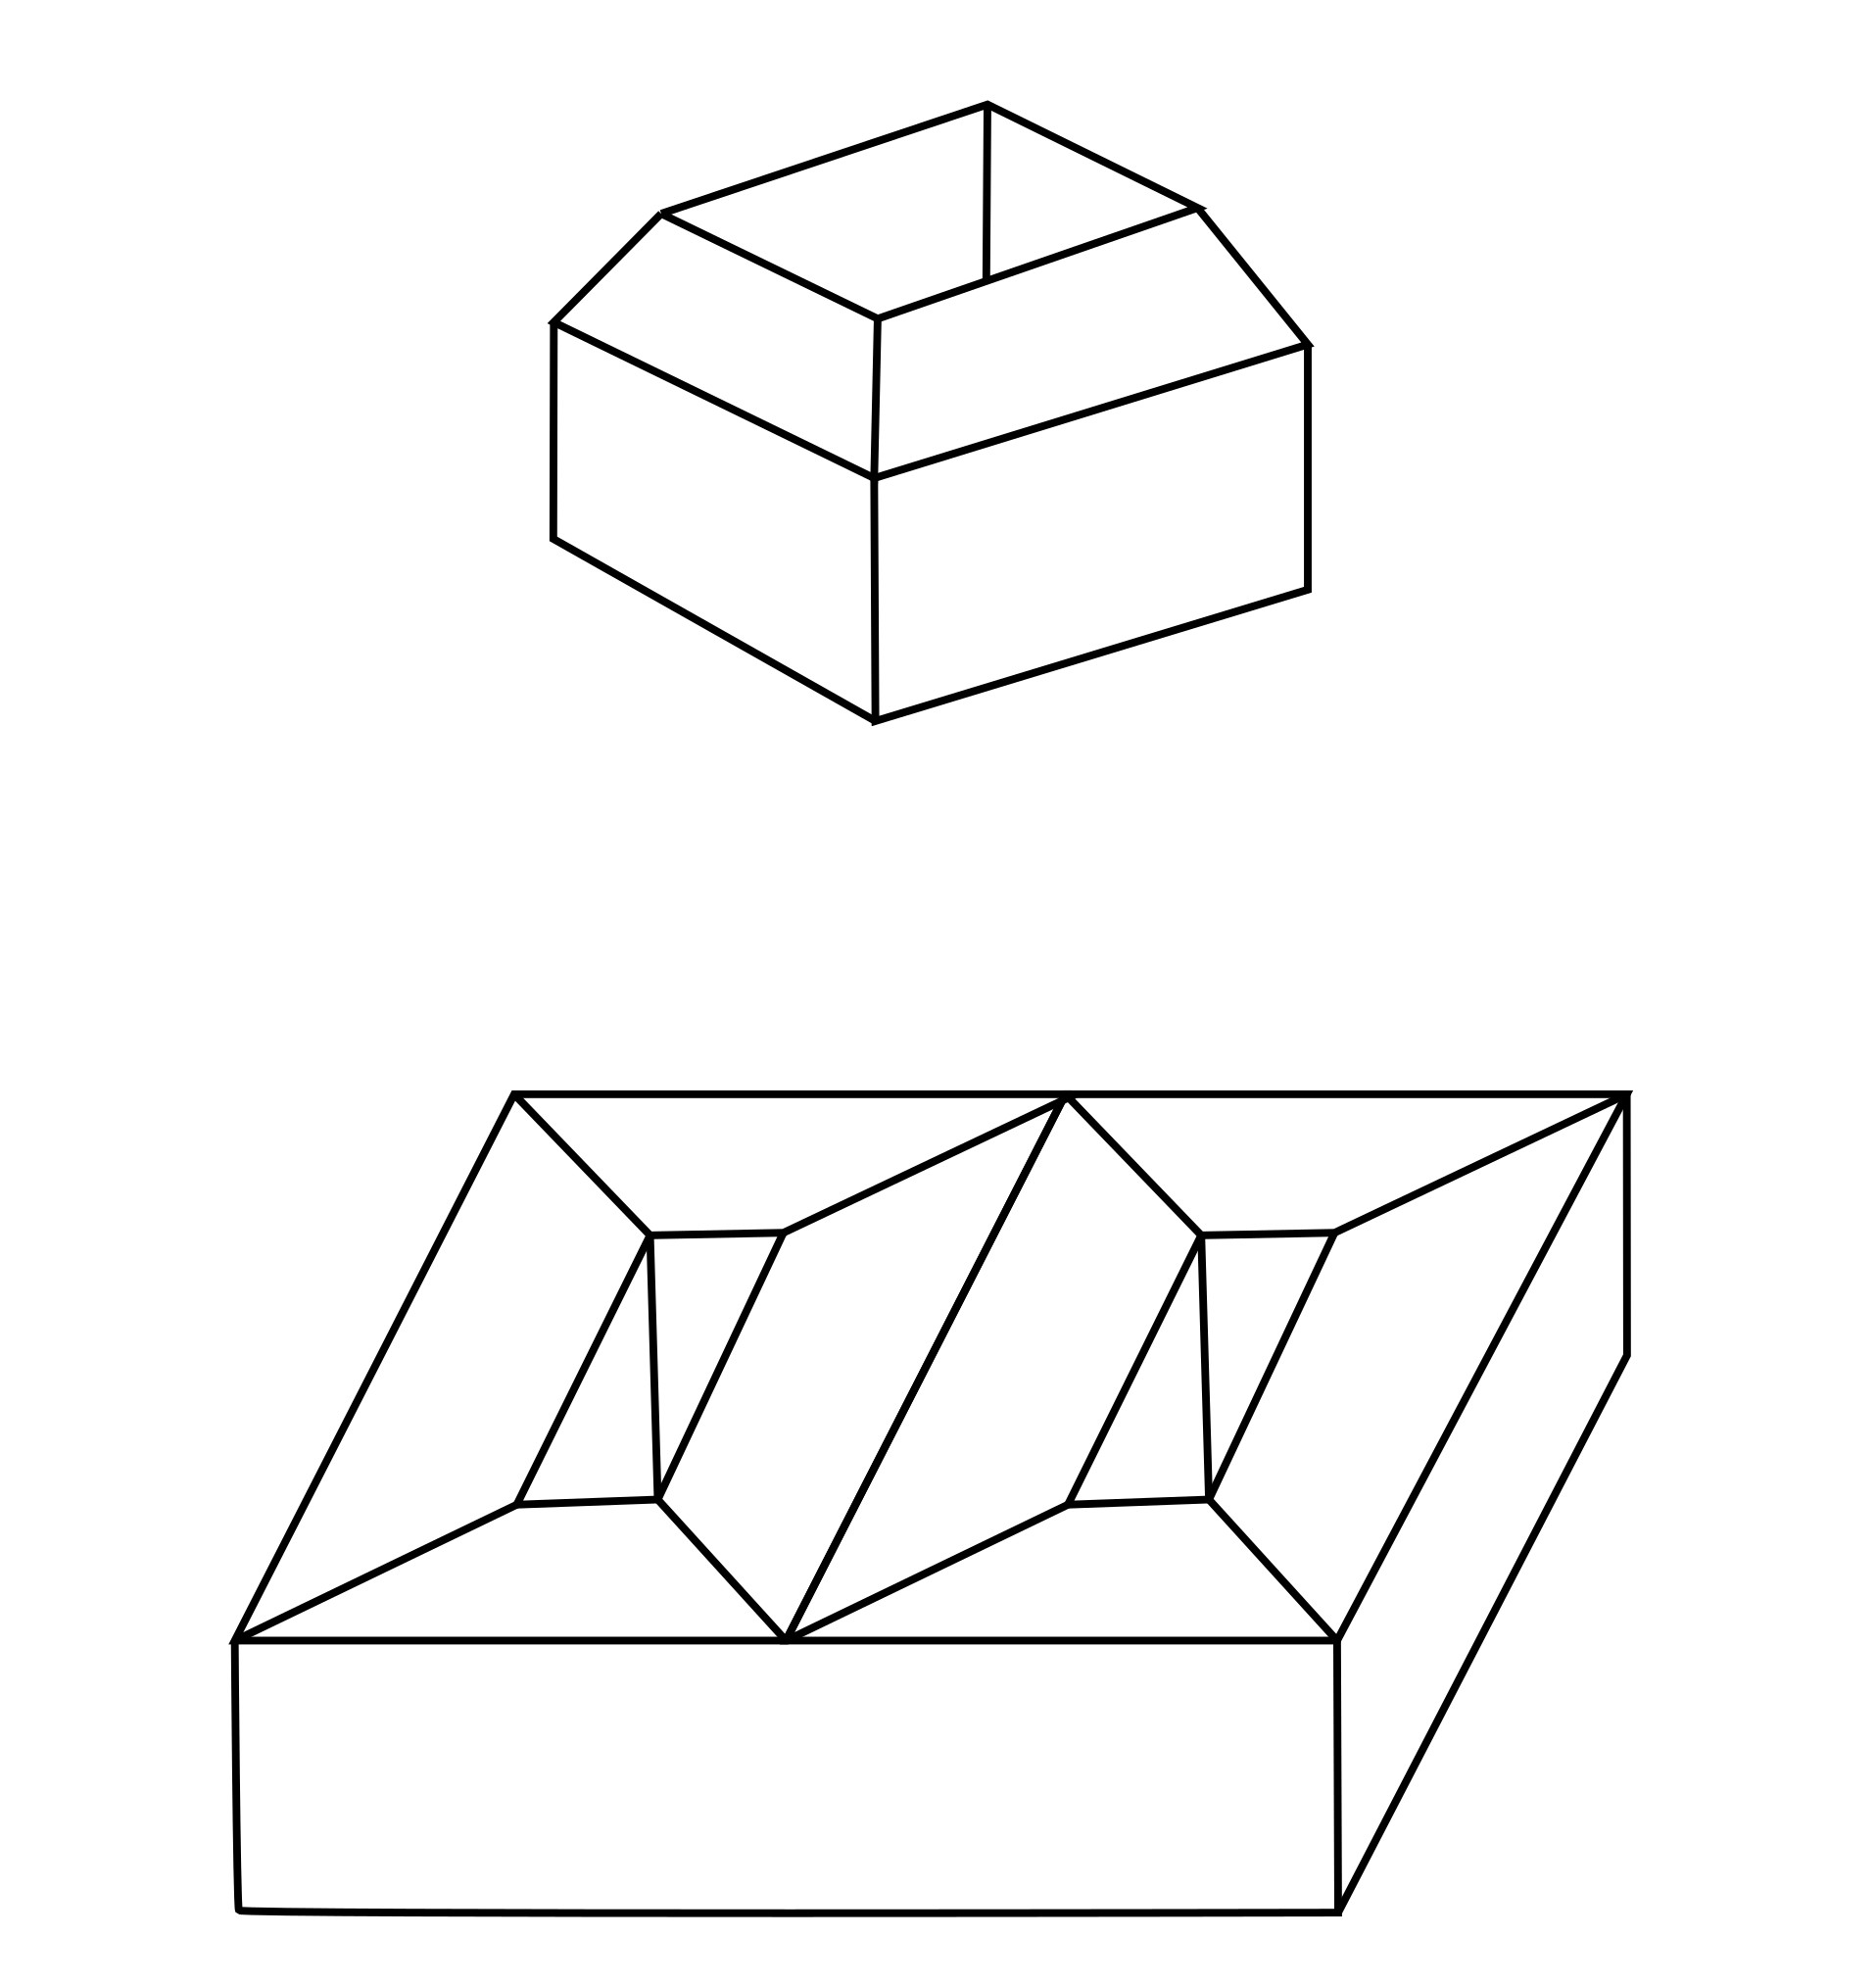
\includegraphics[width=8cm]{Img/GEO/geo-nosimples.jpg}
\centering
\caption{\textbf{Figura 3.11. \footnotesize{ejemplos de poliedros no simples. No se pueden transformar en una esfera}}}
\end{figure}

Para proceder a la clasificación de los poliedros se recurre al concepto de \textbf{número de conectividad (n)}. Si la superficie de un poliedro se puede dividir en dos regiones separadas mediante un camino cerrado trazado a lo largo de sus aristas, decimos que tiene conectividad $n = 0$. Esto es así porque una esfera se puede dividir en dos partes, por cualquier camino cerrado que tracemos sobre su superficie. Se considera que la conectividad de la esfera es 0 $(n = 0)$.\vskip
De esto se obtiene un resultado: \textit{cualquier poliedro cuya conectividad sea 0 puede ser transformado en una esfera}. En la figura 13 hay caminos cerrados que no dividen a la superficie del poliedro en dos partes separadas. A estos poliedros se les asigna un número de conectividad mayor que 0.
Formalmente se define el \textit{número de conectividad como el máximo número de bucles distintos con o sin puntos comunes (intersecciones) que se puedan trazar sobre un poliedro, sin que se divida su superficie en dos regiones separadas}.
Se puede generalizar la fórmula de Euler a poliedros de cualquier número de conectividad n:
$$V - A + C = 2 - n$$
Asimismo, se define el grado $``g”$ de un poliedro de la misma forma que su número de conectividad, pero sin que los bucles se intersequen. La ecuación de Euler, generalizada a poliedros de cualquier grado g es:
$$V - A + C = 2 - 2g$$
de donde se deduce que $2g = n$.
Estas fórmulas son útiles porque partiendo del número de aristas, vértices y caras del poliedro, se puede saber su número de conectividad y el grado
$$n = -V + A - C + 2$$
$$g = \frac{(-V + A - C + 2)}{2}$$
De este modo se sabe si los poliedros equivalen topológicamente a una esfera, a un toro, etc.

\textbf{Curvatura de los modelos poliédricos}\vskip
Toda la curvatura de las superficies de caras planas se concentra en los vértices, lo que facilita el cálculo la curvatura total \textbf{(K)}. Sólo necesitamos sumar el ángulo de exceso de los pequeños caminos alrededor de cada vértice, es decir,
$$
K = \sum_{i=1}^{v}E_{i}
$$
donde $E_i$ es el exceso del camino alrededor del vértice $i$, y $v$ el número de vértices del poliedro.
Recordando que $T + E = 2\pi$ la ecuación anterior queda:
$$
K = \sum_{i=1}^{v}(2\pi - T_i)
$$
donde $T_i$ es el \textit{}giro total del camino alrededor del vértice $i$. Sacando el $2\pi$ fuera del sumatorio se tiene
$$
K = 2\pi V - \sum_{i=1}^{v}( T_i)
$$

Teniendo en cuenta que el giro total del camino alrededor del vértice \textit{$i$ $(Ti)$ es igual a la suma de todos los ángulo interiores de dicho vértice}, la expresión anterior se puede expresar más claramente si se agrupan los ángulos interiores por caras, aprovechando la propiedad asociativa de la suma.

$$
K = 2\pi V - \sum_{i=1}^{C}C_i
$$

donde $ci$ es la suma de los ángulos interiores de la cara $i$ y $C$ es el total de caras del poliedro.
Este es un resultado sorprendente porque podemos calcular el segundo término sin saber cómo están unidas las distintas aristas. Por tanto, si conocemos todas las caras del poliedro y conocemos $V$, podemos calcular la curvatura total sin saber nada sobre las relaciones entre las aristas y las caras.\vskip
Para poliedros cuyas caras sean cuadrados la fórmula es todavía más simple, ya que la suma de los ángulos interiores de cualquier cara es $2\pi$.\vskip 
Por tanto, $K = 2\pi V - 2\pi C$ ó $K = 2\pi (V - C)$. Ver que esta ecuación para calcular la curvatura total no depende de los ángulos para nada.
La expresión anterior aún se puede generalizar más. Partiendo de la Ec. 13, se puede demostrar que la suma
$\sum_{{i=1}^{C}} C_i$
puede expresarse independientemente de los valores particulares de los ángulos; solamente se necesita conocer el número total de caras, vértices y aristas. Según esto, para una superficie de caras planas cerrada con $V$ vértices, $A$ aristas y $C$ caras, la \textit{curvatura total} es $$K = 2\pi (V - A + C)$$

A la cantidad $(V - A + C)$ se le llama \textit{característica de Euler} de una superficie y se denota con la letra griega
$\chi$ (chi). Usando esta notación, rescribimos la fórmula de la curvatura como
$$K = 2\pi \chi$$

La Ec. 15 muestra que, para cualquier superficie cerrada, la curvatura total y la característica de Euler están relacionadas. Esto constituye el \textbf{teorema de Gauss-Bonnet}, y \textit{puede ser aplicado a todo tipo de superficies cerradas}, no sólo a las de caras planas, ya que la característica de Euler es una constante topológica al igual que a curvatura total. Este teorema es de suma importancia para la validación de las redes trazadas sobre superficies cerradas: \textit{todas las infinitas redes diferentes que es posible trazar sobre una superficie cerrada poseen la misma característica de Euler}.
Este teorema proporciona resultados muy importantes, ya que además de ser un medio muy útil para poder calcular la curvatura total de las superficies cerradas, da una relación entre una cantidad definida en términos topológicos, como es la característica de Euler, con otra definida en términos geométricos, como es la curvatura total.


\textbf{Representación topológica de los poliedros.}\vskip
Uno de los puntos clave en el modelado con poliedros es cómo se ha de registrar su información topológica, es decir, las relaciones entre los vértices, aristas y caras que los definen.
La forma más simple y directa para representar los poliedros consiste en describir cada cara por separado, señalando explícitamente cómo han de unirse. Este método de representación se conoce como \textbf{atlas}. La figura 14 muestra el atlas de un cubo.

\begin{figure}[h]
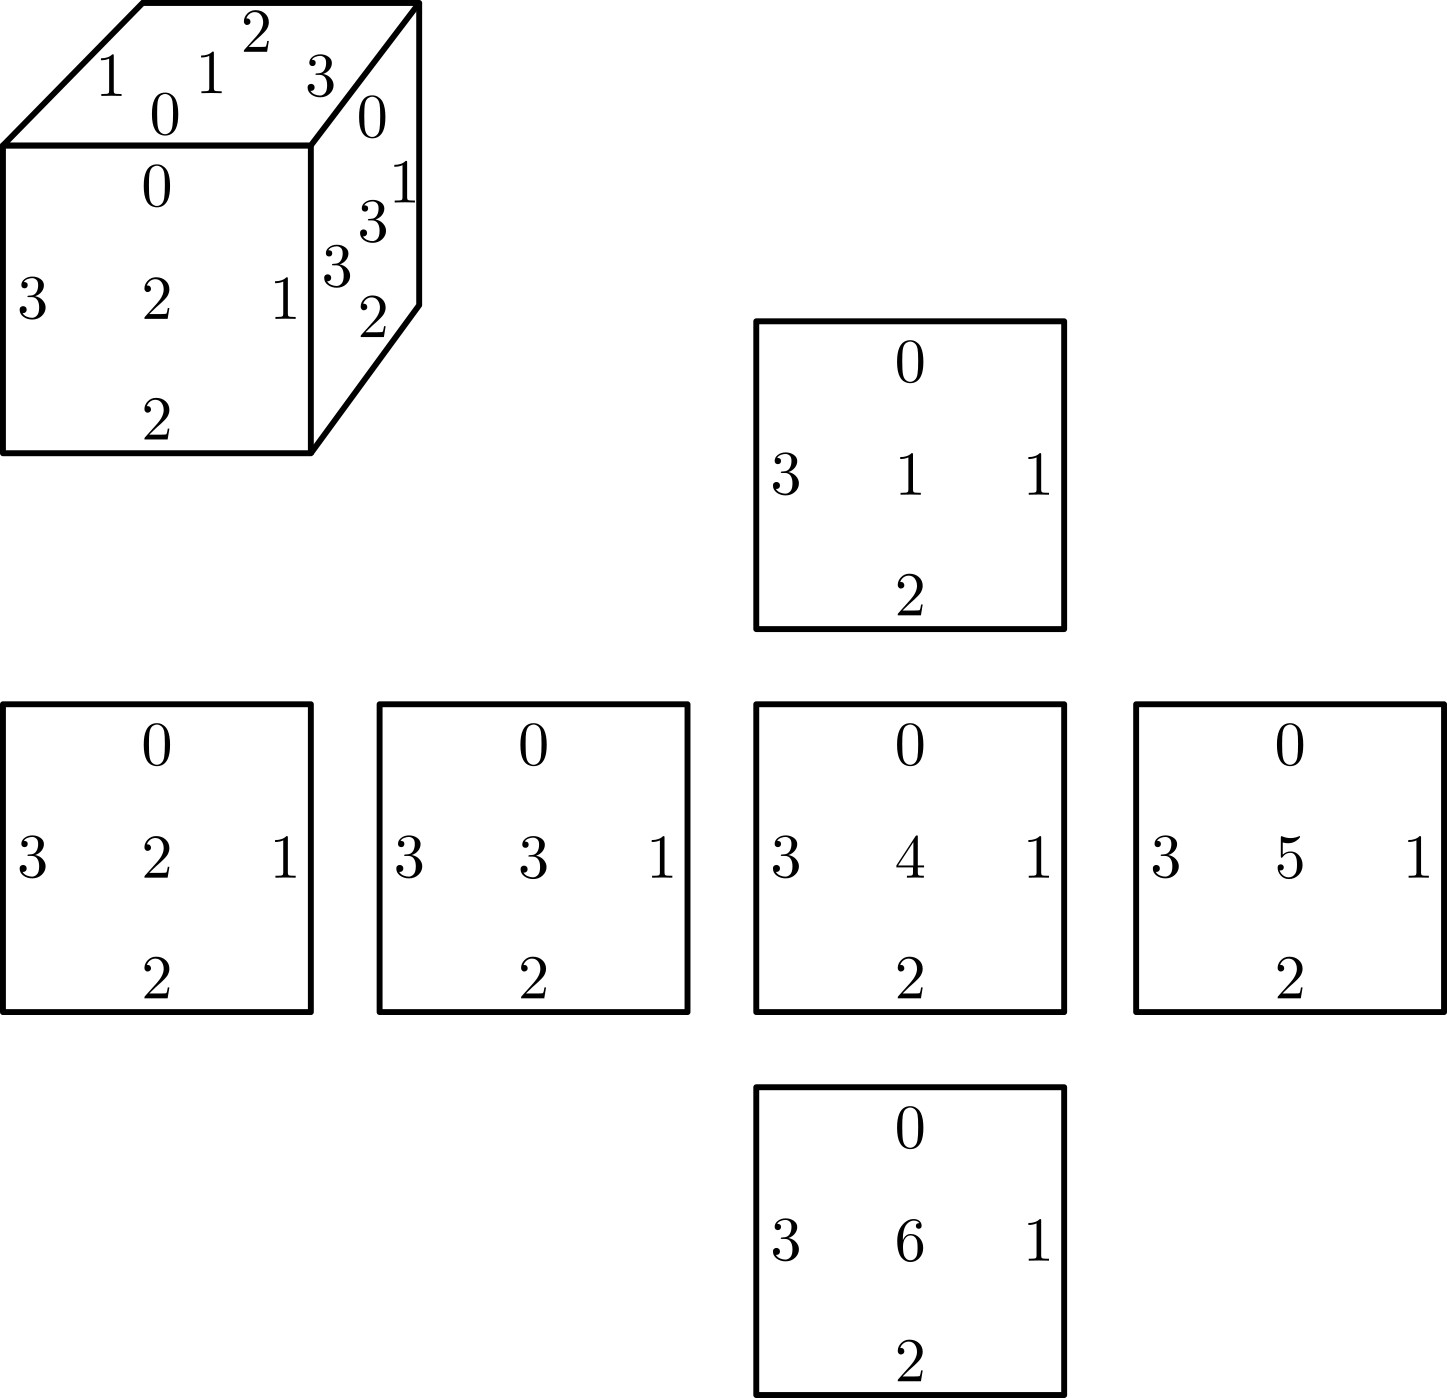
\includegraphics[width=8cm]{Img/GEO/geo-atlas0.jpg}
\centering
\caption{\textbf{Figura 3.11. \footnotesize{atlas de un cubo}}}
\end{figure}

Cada eje se etiqueta con un par de números indicando la cara y el número de la arista de la cara. Así el par (1,0) se interpreta como la arista 0 de la cara 1. Cada unión de dos aristas se especificará por dos pares de números, identificando las aristas que se unen. De esta forma, el atlas formado queda como siguiente:


$$
\begin{array}{c@{}c@{}c@{}c}
 \begin{array}{cc}
         [(1,0) & (2,0)]
  \end{array} & \begin{array}{cc}
         [(1,1) & (5,0)]
  \end{array} & \begin{array}{cc}
         [(1,2) & (4,0)]
  \end{array} &
  \begin{array}{cc}
         [(1,3) & (3,0)] 
  \end{array}
  \\
  \begin{array}{cc}
         [(2,1) & (3,3)]
  \end{array} & \begin{array}{cc}
         [(2,3) & (6,2)]
  \end{array} & \begin{array}{cc}
         [(2,3) & (5,1)] 
  \end{array} &
  \begin{array}{cc}
         [(3,1) & (4,3)]
  \end{array}
  \\
  \begin{array}{cc}
         [(3,2) & (6,3)]
  \end{array} & \begin{array}{cc}
         [(4,1) & (5,3)]
  \end{array} & \begin{array}{cc}
         [(4,2) & (6,0)] 
  \end{array} &
  \begin{array}{cc}
         [(5,2) & (6,1)] 
  \end{array}
\end{array}
$$   

\begin{center}
\textbf{Tabla 3.11. \footnotesize{representación matricial del atlas}}
\end{center}

Además de especificar qué aristas están unidas, se ha de decir cómo unirlas. La figura 15 muestra dos formas diferentes de unir un par de aristas. La primera, mostrada a la izquierda, es la unión con \textit{orientación conservadora}, y la segunda tiene \textit{orientación inversora}. Para unir esas dos aristas hay que hacer coincidir los números de cada una de ellas. Si se hace mediante la orientación conservadora se obtiene un cilindro y una \textit{cinta de Moebius\footnote{La cinta de Möbius o Moebius es una superficie con una sola cara y un solo borde. Tiene la propiedad matemática de ser un objeto no orientable.}} con la orientación inversora.

\begin{figure}[h]
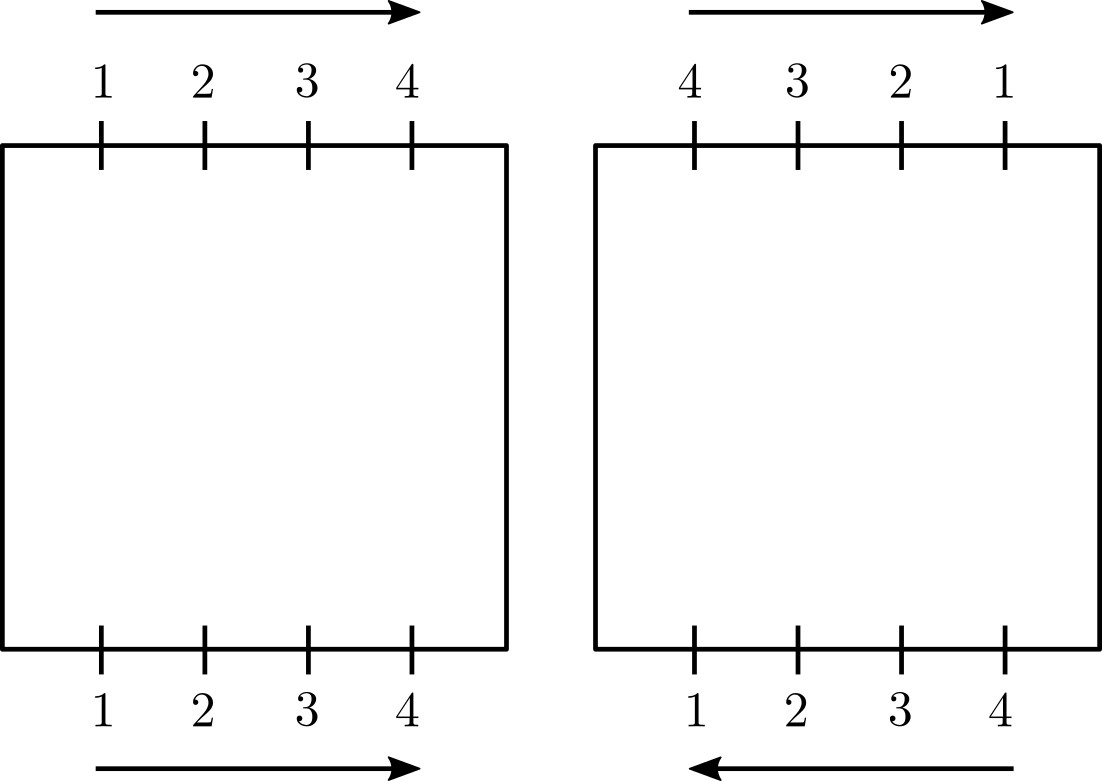
\includegraphics[width=8cm]{Img/GEO/geo-atlas1.jpg}
\centering
\caption{\textbf{Figura 3.11. \footnotesize{orientaciones conservadora e inversora}}}
\end{figure}

Para especificar en el atlas de qué forma se van a unir las aristas, utilizamos la \textit{paridad de transición} que es $\pm 1$, unida al par de aristas. La figura 16 presenta varios ejemplos de un esquema de notación que incluye el número de paridad de transición

\begin{figure}[h]
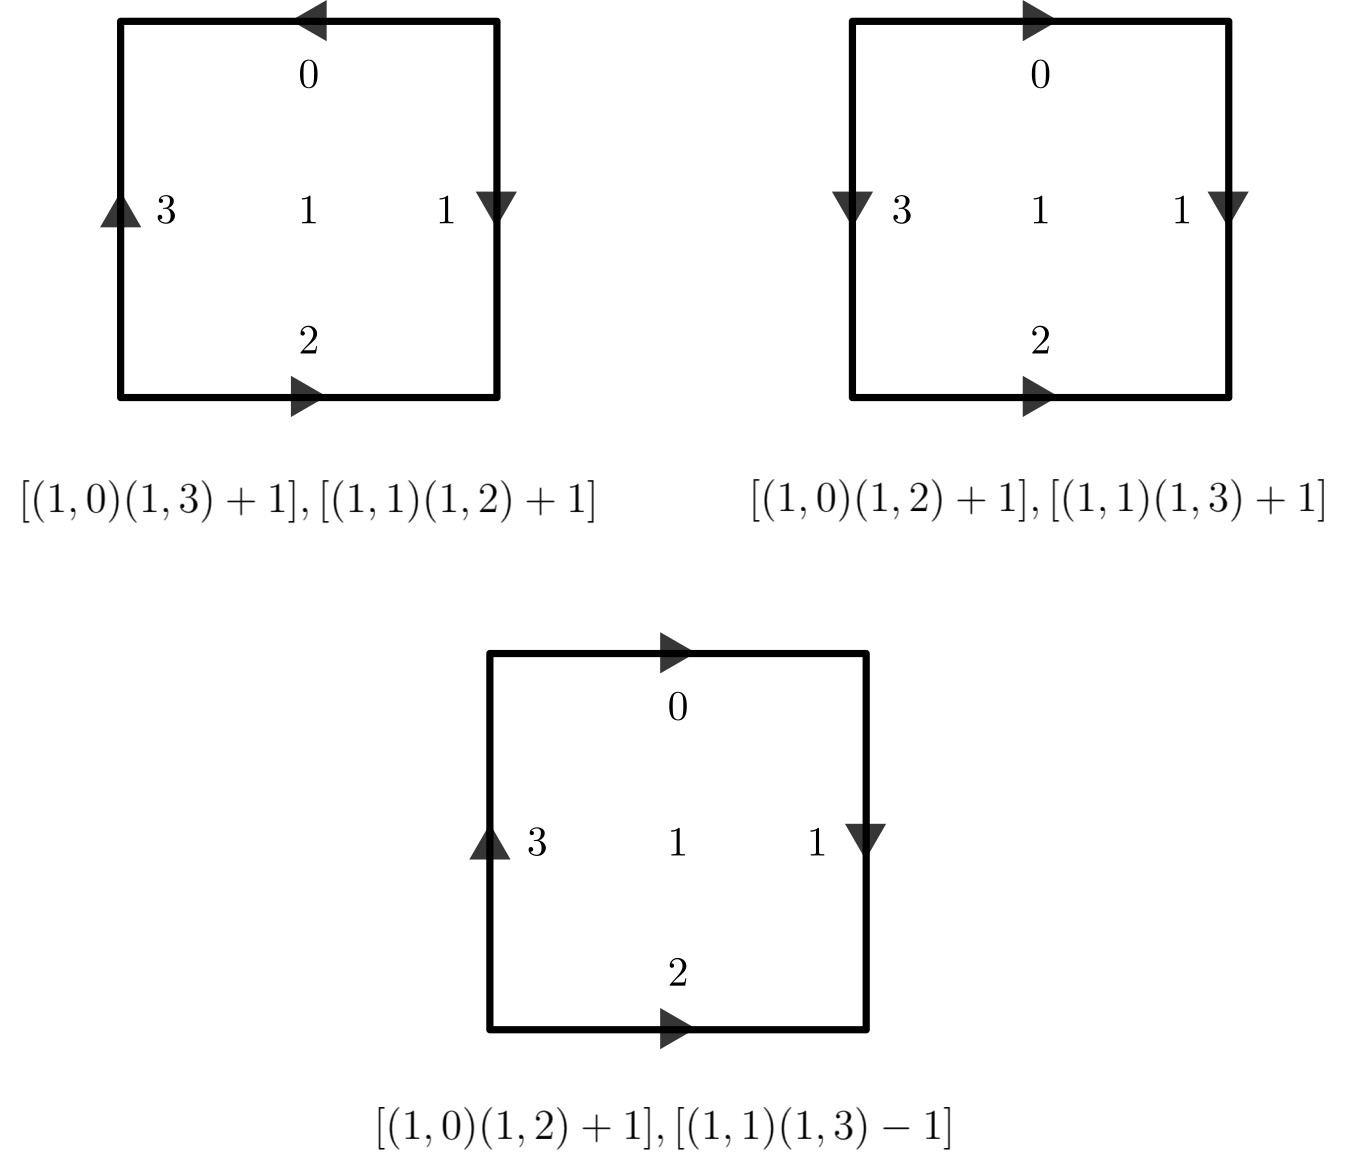
\includegraphics[width=11cm]{Img/GEO/geo-atlas2.jpg}
\centering
\caption{\textbf{Figura 3.11. \footnotesize{atlas y paridad de transición de una esfera, un toro y una botella de Klein.}}}
\end{figure}


\textbf{A) Superficies Orientables y No Orientables} \vskip
Si utilizamos uniones no conservadoras en un atlas podemos conseguir algunas curiosidades matemáticas llamadas \textit{superficies no orientables}, como la \textit{cinta de Moebius} y la \textit{botella de Klein}\footnote{En topología, una botella de Klein es una superficie no orientable abierta cuya característica de Euler es igual a 0 ; no tiene interior ni exterior.} (figura 17). La cinta de Moebius posee una curiosa particularidad. Si se recorre la cinta comenzando en un punto cualquiera, y se da una vuelta completa, como se trata de una cinta bidimensional, cuando se llegue al punto de partida se observará que la derecha e izquierda están intercambiadas. Este tipo de superficies se llaman \textbf{no orientables} y se producen al efectuar uniones no conservadoras entre sus aristas. Por el contrario, si en la superficie nunca se intercambian la izquierda y derecha, entonces se dice que la superficie es \textbf{orientable}.

\begin{figure}[h]
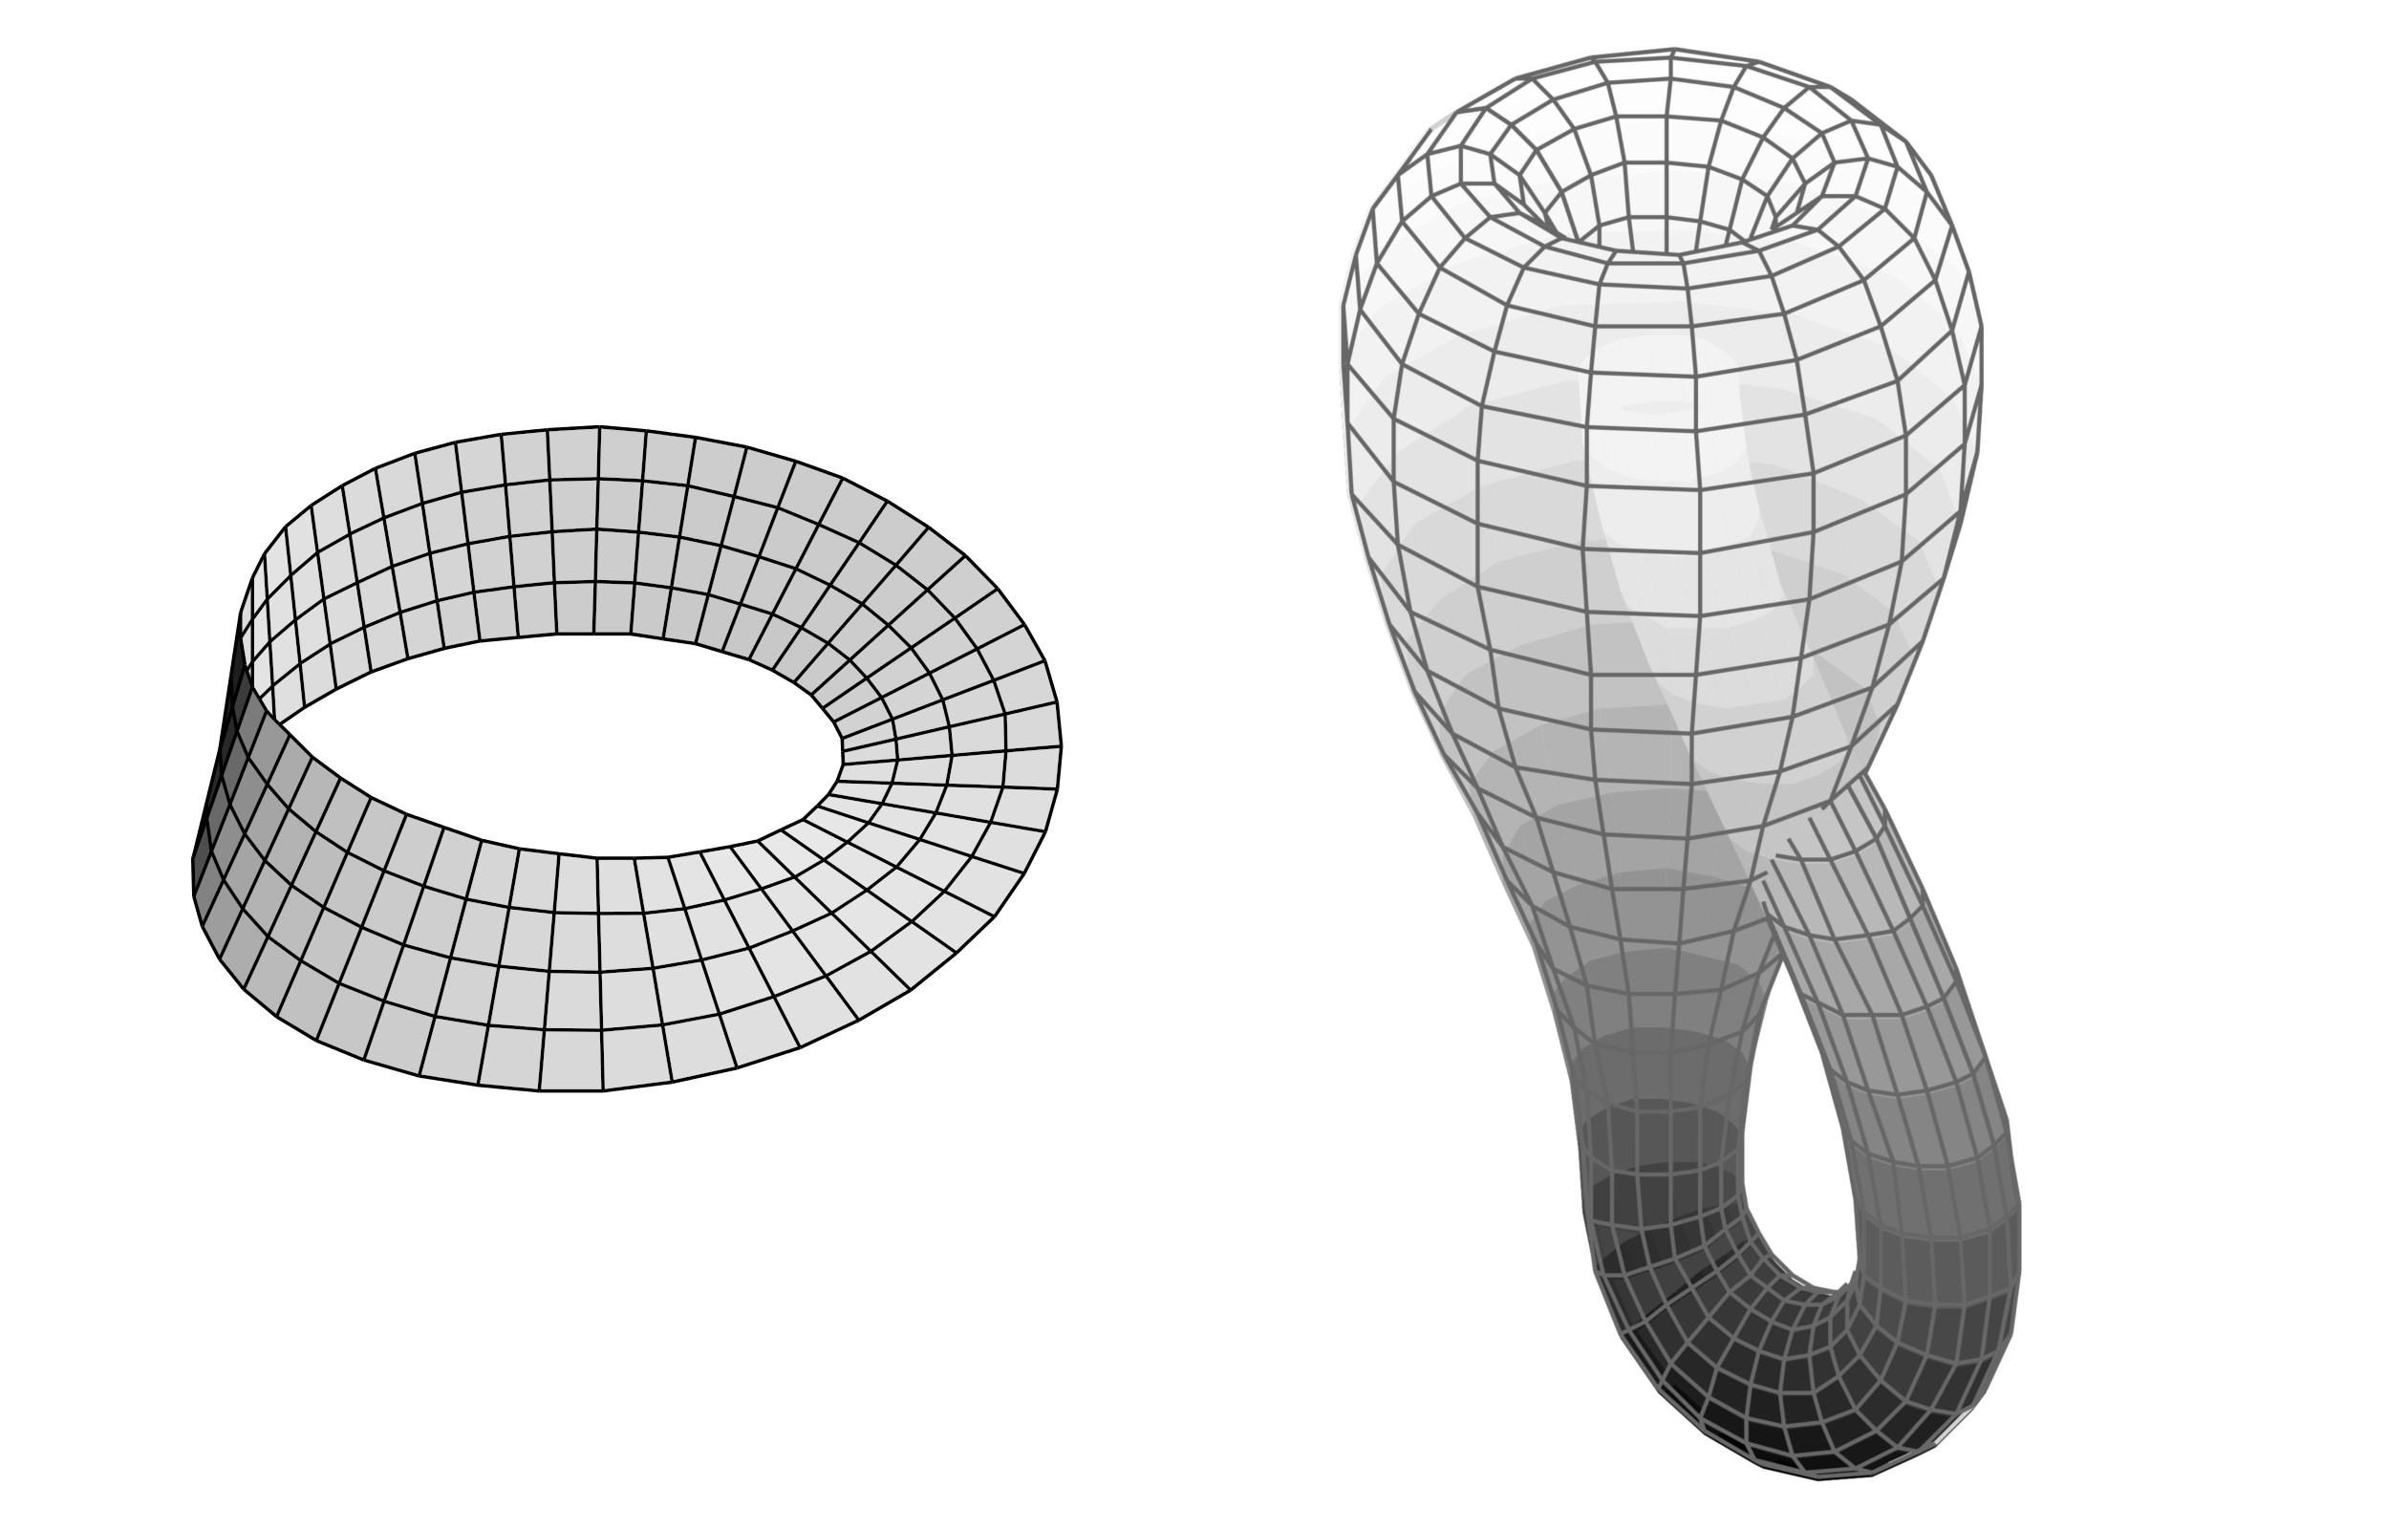
\includegraphics[width=14cm]{Img/GEO/geo-mobius.jpg}
\centering
\caption{\textbf{Figura 3.11. \footnotesize{Cinta de Moebius y Botella de Klein}}}
\end{figure}

Habíamos visto que para que cualquier superficie cerrada tridimensional sea consistente, debe ser topológicamente equivalente a una esfera con $g$ asas. Ahora se añade otra condición más: \textit{debe ser orientable}.
Si partimos de una cinta de Moebius y la cerramos aplicando una orientación conservadora, obtenemos otra superficie no orientable llamada botella de Klein, que no se puede construir en un espacio tridimensional sin que se auto interseque.


\subsubsection{ Objetos de Euler }
A los objetos cerrados tridimensionales de orden $g \geq 0 $ que verifican ciertos
requisitos de construcción, se les denomina objetos de Euler. Dichas normas son:

\begin{itemize}
\item Todas sus caras (curvas o planas) han de ser discos topológicos. 
\item Cada arista une sólo dos caras y todas finalizan en un vértice en
cada extremo.
\item Por lo menos tres aristas se unen en un vértice. 
\end{itemize}

En los objetos de Euler se cumple que:


\begin{equation}
V - A + C  = 2(S-P)
\end{equation}

\begin{description}
\item $S$: número de superficies inconexas del objeto.
\item $P$: total de pasajes (túneles) en el objeto.
\end{description}

Como el número de pasajes en un objeto es igual al total de ``asas” o agujeros que posea, ocurre que en la ecuación anterior $P$ es igual al orden del objeto $(P = g)$.\vskip
Para entender mejor el significado de $S$, la figura 18 muestra tres objetos eulerianos, con una, dos y tres superficies inconexas.

\begin{figure}[h]
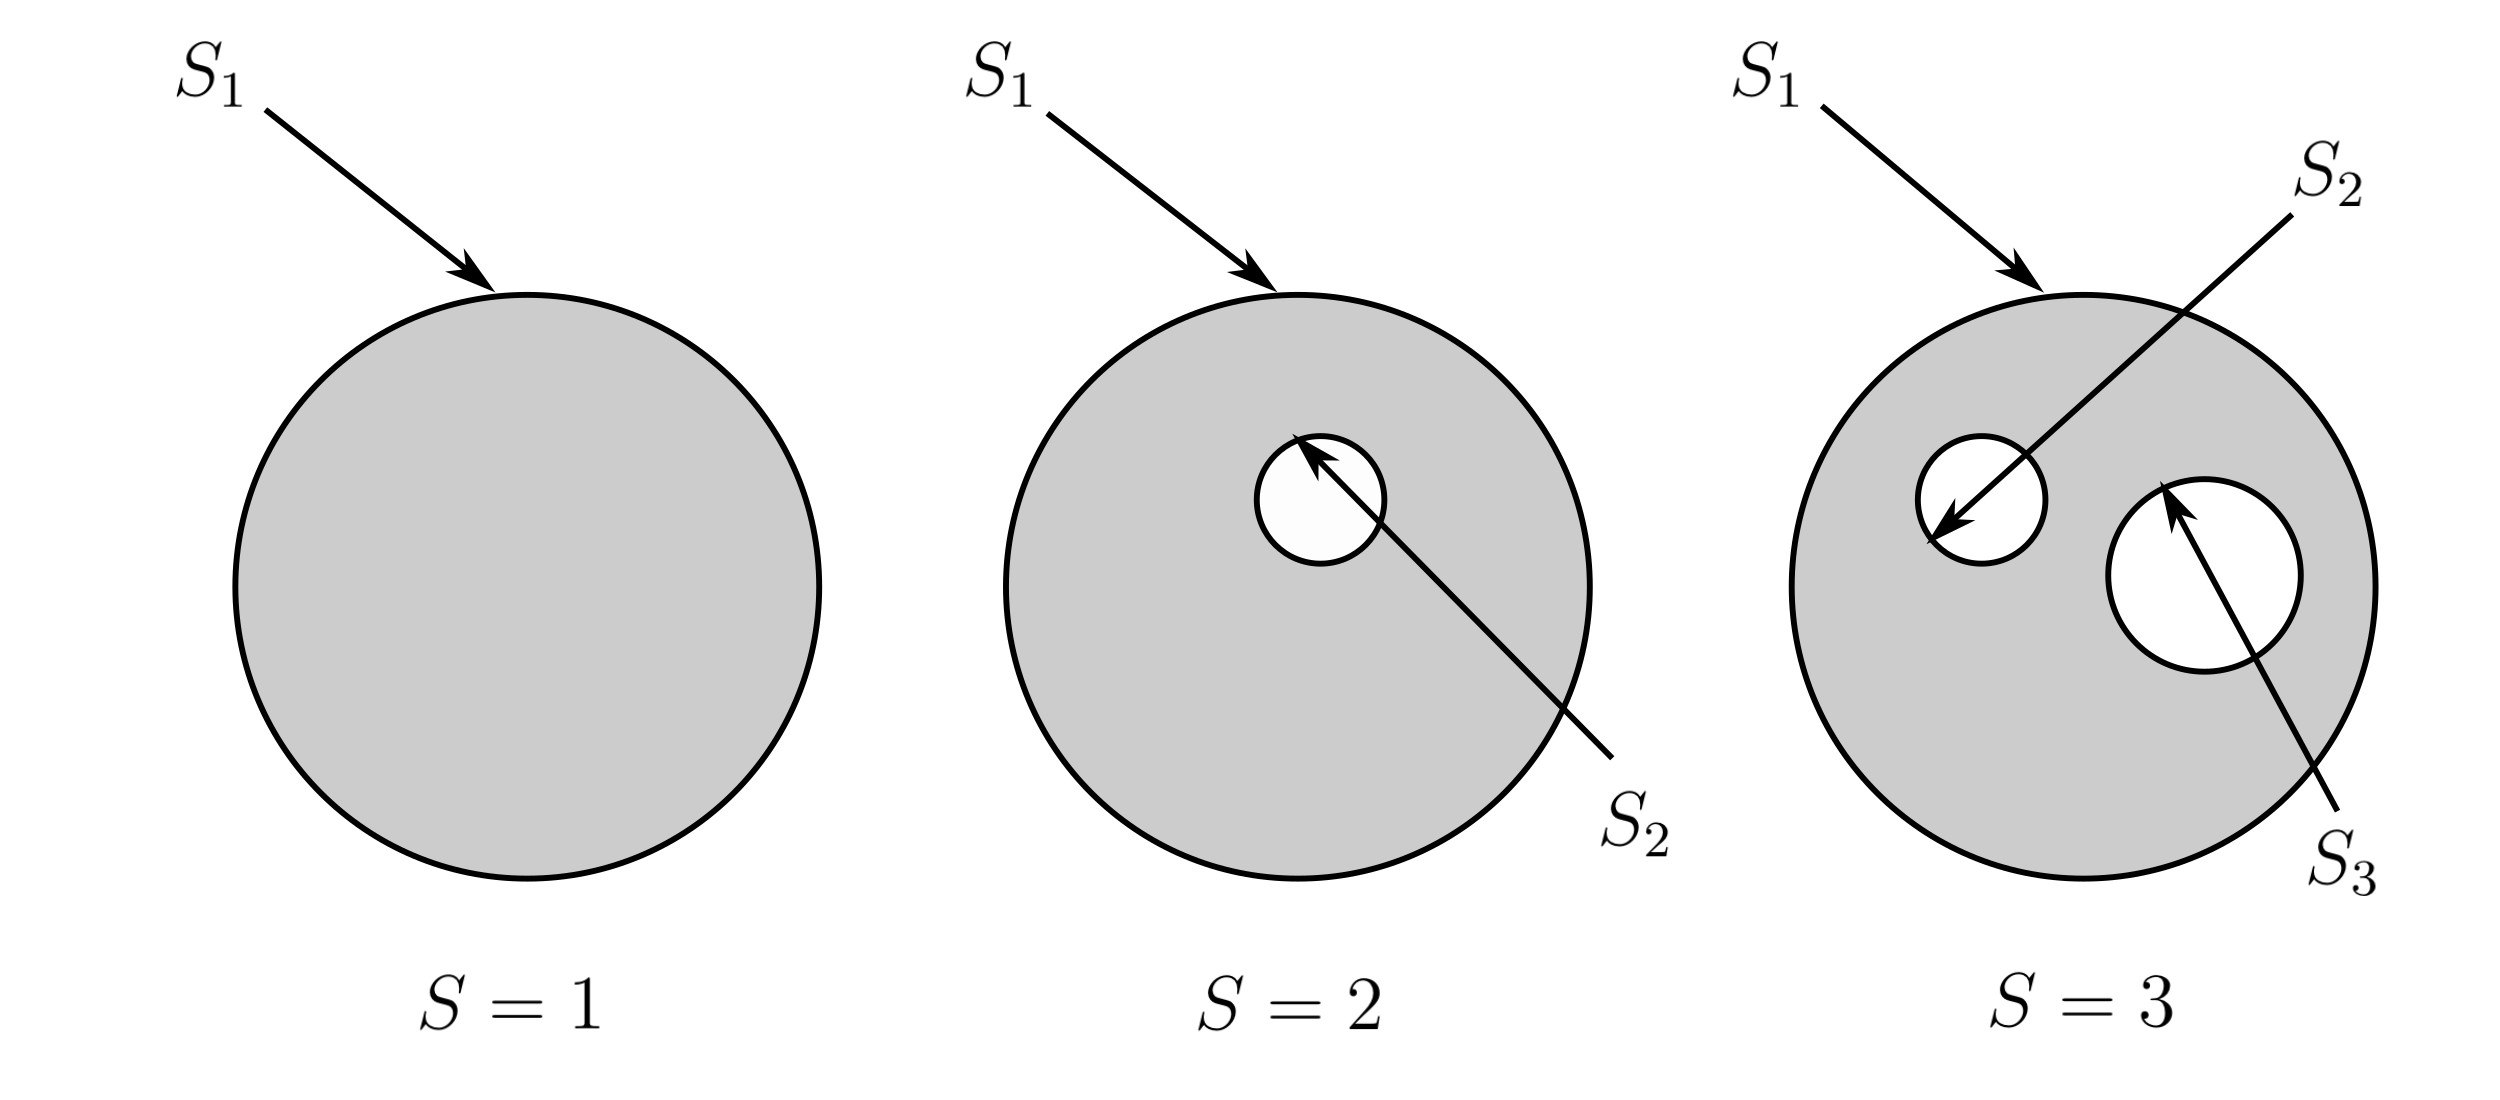
\includegraphics[width=12cm]{Img/GEO/geo-euler0.jpg}
\centering
\caption{\textbf{Figura 3.11. \footnotesize{Objetos de Euler con diferentes valores de $S$}}}
\end{figure}

En la figura 3.13 se pueden ver algunos ejemplos de objetos eulerianos, cuando $S = 1$ y $P = 0$. Ver que en este caso la Ec. 16 se reduce a la ecuación de Euler.

\begin{figure}[h]
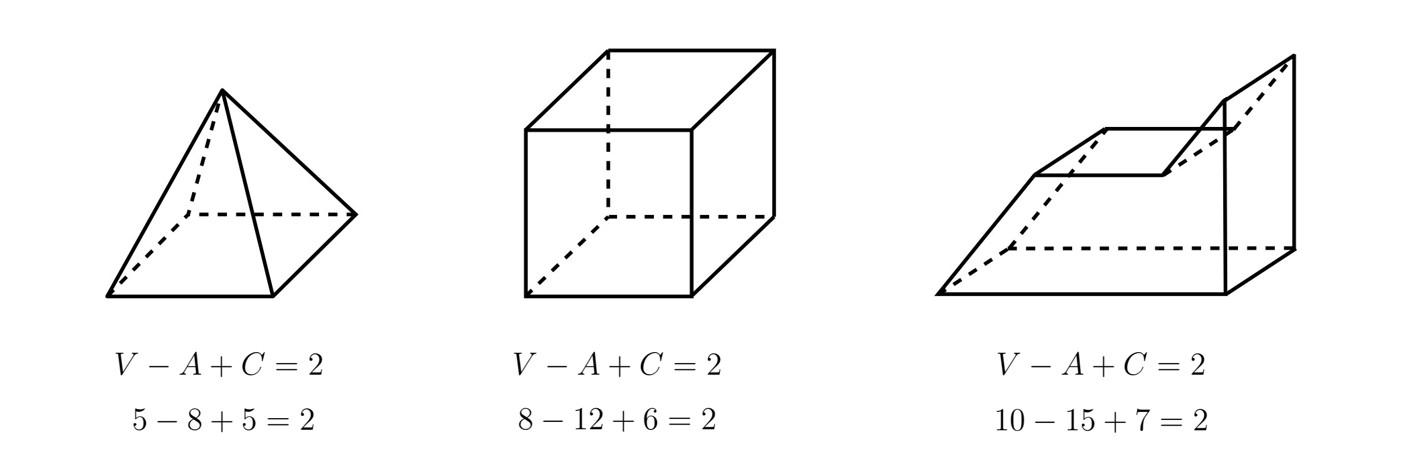
\includegraphics[width=14cm]{Img/GEO/geo-euler1.jpg}
\centering
\caption{\textbf{Figura 3.11. \footnotesize{Ejemplos de objetos de Euler}}}
\end{figure}


En la figura 20 hay otros dos objetos de Euler. El izquierdo es de grado 1, ya que tiene un túnel que lo cruza; el otro, aunque posee una cavidad, ésta no llega a atravesar el modelo. Por tanto, se trata de un objeto topológicamente equivalente a una esfera, es decir, de grado 0.

\begin{figure}[h]
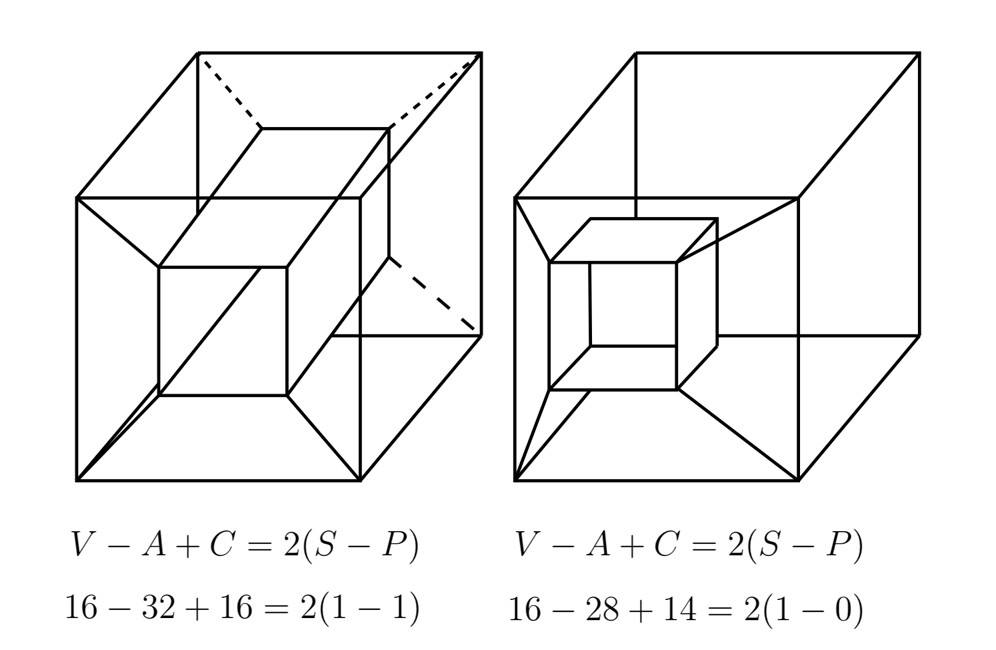
\includegraphics[width=8cm]{Img/GEO/geo-euler2.jpg}
\centering
\caption{\textbf{Figura 3.11. \footnotesize{Objetos eulerianos de grado 1 y 0, respectivamente}}}
\end{figure}


\textbf{ Operadores de Euler.}\vskip
Los \textbf{operadores de Euler} \textit{permiten crear y transformar objetos de Euler, en nuevos objetos (también eulerianos)} mediante la adición o eliminación de caras, aristas y vértices. Dichos operadores son especialmente útiles en la creación y transformación de los modelos poliédricos, ya que directamente generan modelos íntegros, lo que evita (o minimiza) la verificación de la integridad de los modelos. Los operadores de Euler trabajan directamente sobre las estructuras de datos que definen los objetos. Por lo tanto, \textit{un operador de Euler es un proceso} que actúa sobre la base de datos donde está la información de los poliedros que ha de crear o transformar.\vskip
Durante la transformación de un objeto de Euler en otro objeto de Euler, \textit{inevitablemente se producen objetos intermedios que no son de Euler}. Por ejemplo, en la figura 21 podemos ver tres transformaciones realizadas con operadores de Euler. En el primer y segundo caso se han añadido las aristas y vértices suficientes para que los objetos resultantes sigan siendo de Euler. En el caso tercero, aunque cumple la ecuación de Euler, sin embargo, las aristas $(1,5)$ y $(2,5)$ no unen dos caras y, además, del vértice 5 no parten tres aristas, por lo que se trata de un objeto intermedio no euleriano. Éste puede convertirse en euleriano añadiendo dos nuevas aristas, la $(4,5)$ y la $(3,5)$.

\begin{figure}[h]
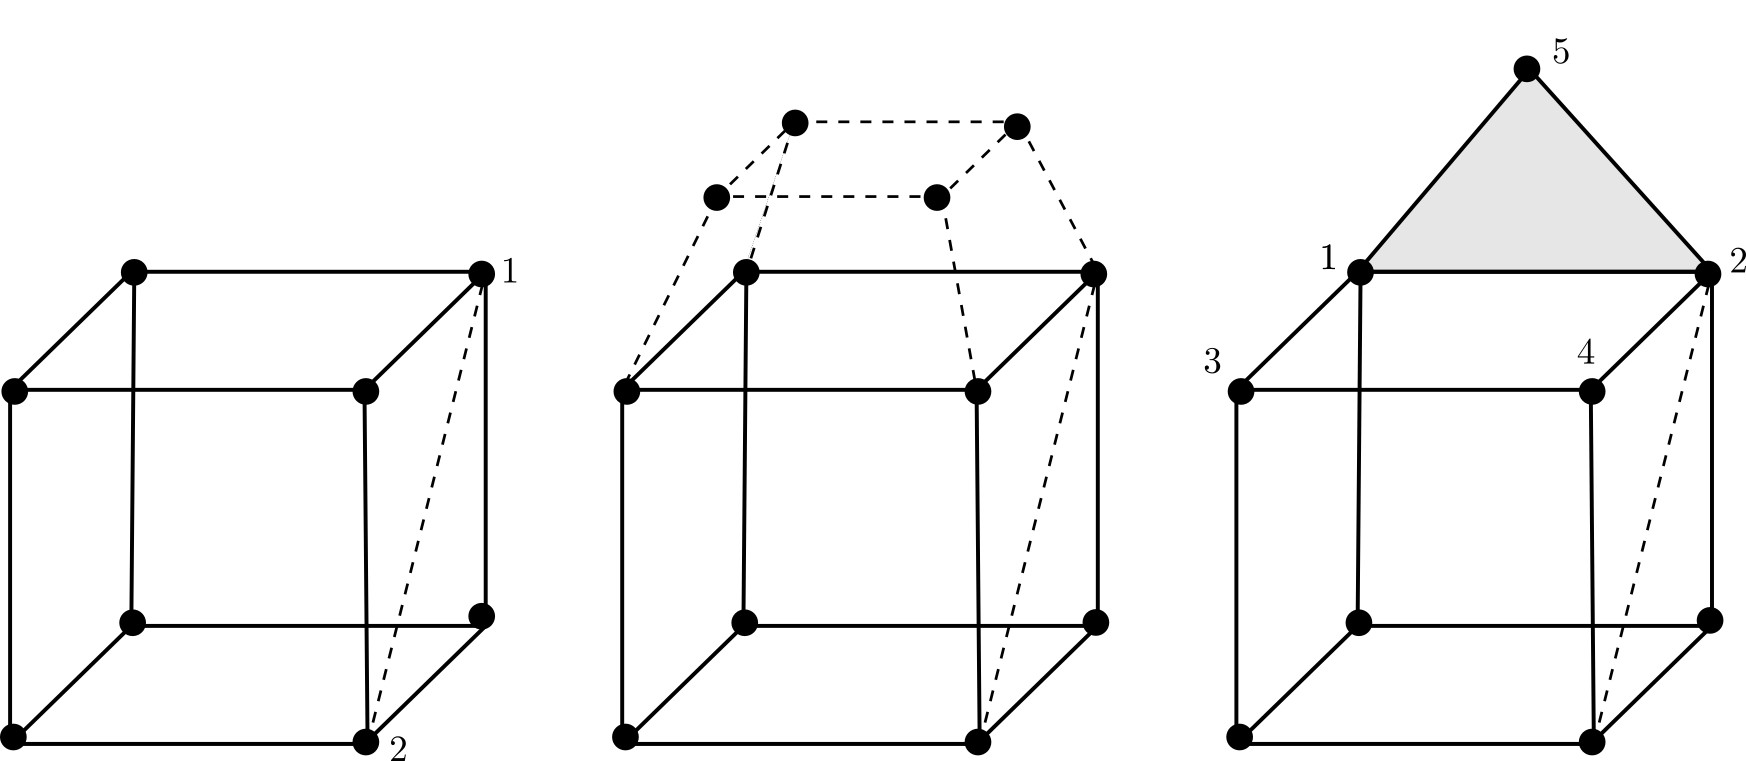
\includegraphics[width=12cm]{Img/GEO/geo-euler3.jpg}
\centering
\caption{\textbf{Figura 3.11. \footnotesize{Operaciones de Euler sobre un cubo.}}}
\end{figure}

A base de añadir o eliminar aristas, vértices y caras, los operadores de Euler sólo pueden transformar los objetos de Euler en otros de la misma familia topológica. Si a partir de un objeto de grado g se pretende obtener otro de grado diferente, entonces no queda más remedio que agujerear alguna superficie (acordarse del proceso de pegado de asas) para poder construir un nuevo pasaje.\vskip
Por lo tanto, para poder cambiar el grado de los objetos, \textit{los operadores de Euler incorporan la posibilidad de añadir o eliminar agujeros a los discos topológicos que configuran los objetos de Euler}. Al agregar un agujero en una cara, se crea un objeto intermedio3 donde se cumple que:

$$V - A + C - O  = 2(S-P)$$

$``O”$ es el total de orificios (agujeros) en las caras. Ver que la ecuación de los objetos eulerianos es un caso particular de ésta, ya que entonces $O = 0$.\vskip
Los sumandos de la izquierda en la expresión $V - A + C  = 2(S-P)$ pueden ser modificados directamente en la estructura de datos, mientras que los de la derecha (S y P) no. Esto significa que si, por ejemplo, se desea transformar un objeto de Euler de modo que el objeto final resultante haya cambiado de familia topológica (variado $g$), es posible conseguirlo añadiendo o eliminando vértices, aristas, caras y/o agujeros en las caras, de forma que al final se cumpla que
$V^\prime - A^\prime + C^\prime - O^\prime  = 2(S^\prime-P^\prime)$

En el ejemplo de la figura 22, vemos un objeto no euleriano con un agujero en una cara y su transformación en uno de Euler. Ver que el hacer agujeros en las caras, no implica necesariamente que el objeto euleriano resultante sea de grado diferente al del objeto original.

\begin{figure}[h]
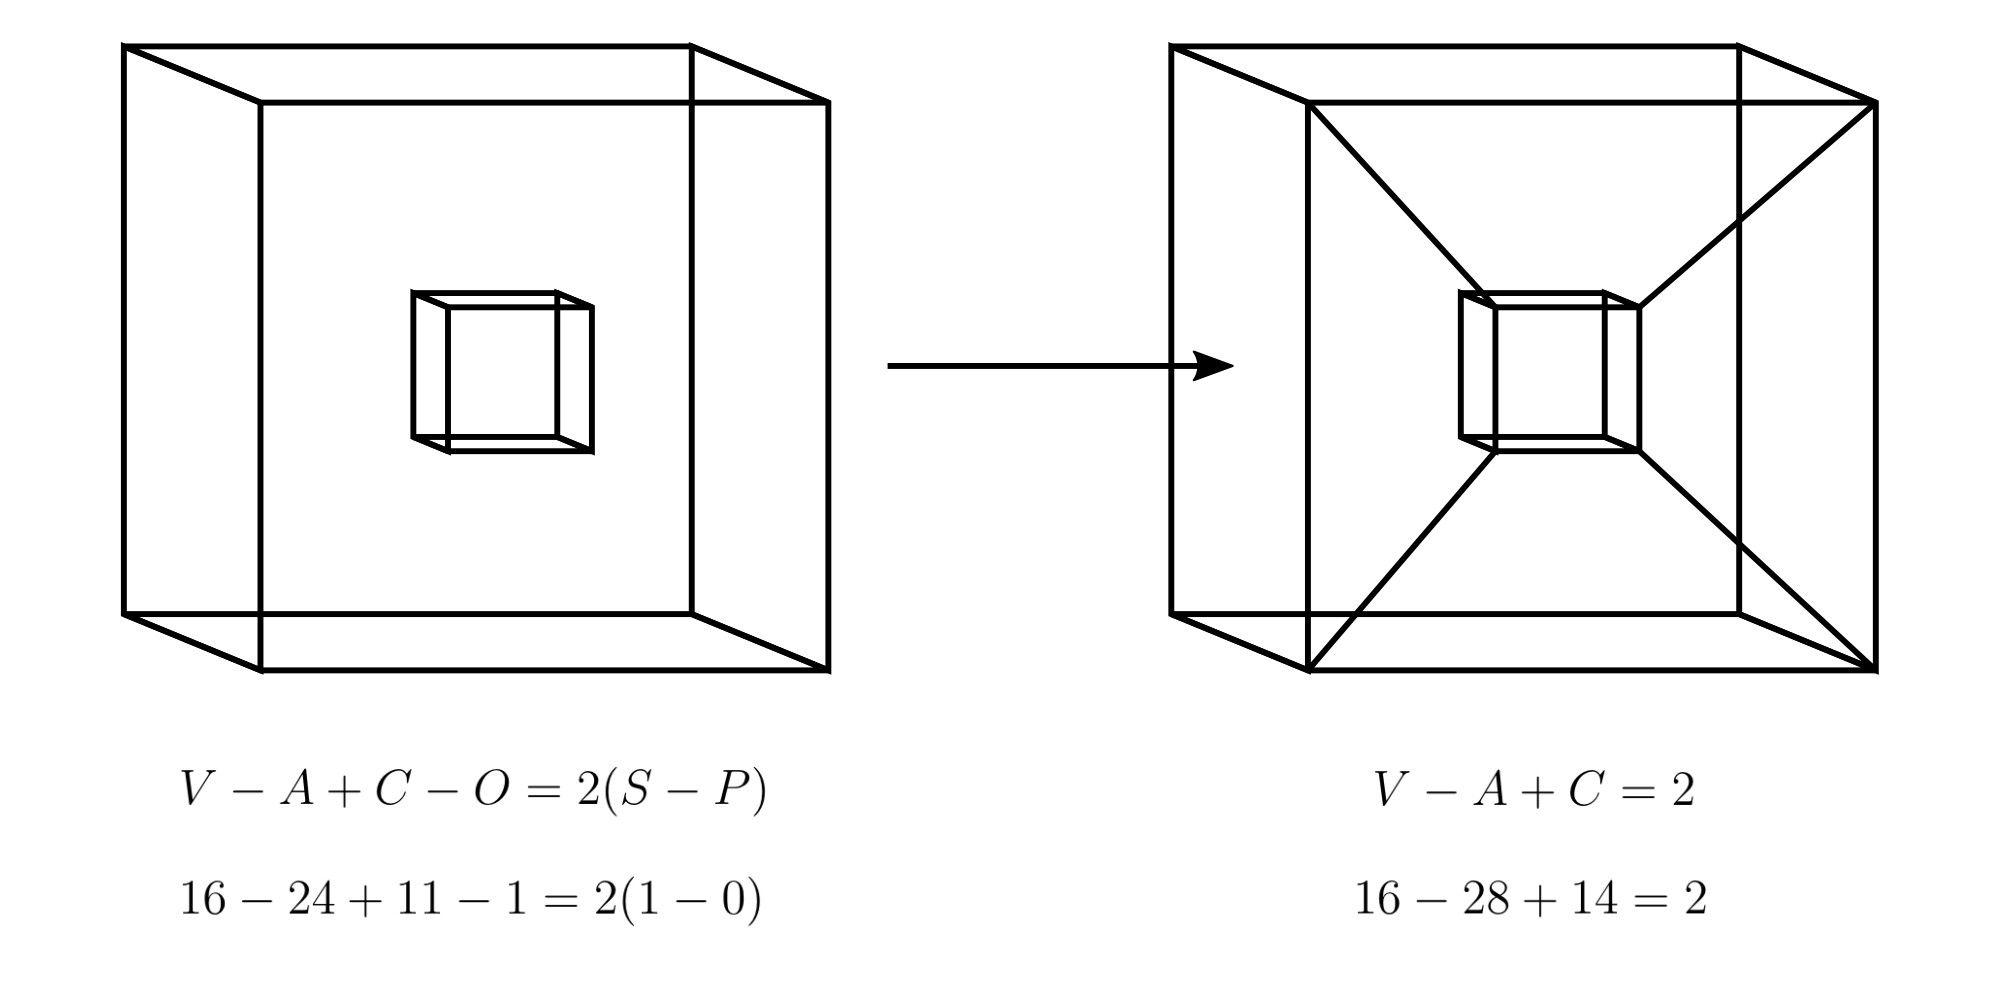
\includegraphics[width=12cm]{Img/GEO/geo-euler4.jpg}
\centering
\caption{\textbf{Figura 3.11. \footnotesize{Transformación de un objeto no euleriano en otro de Euler.}}}
\end{figure}

\textbf{A) Elección de los operadores de Euler}\vskip

Dado que interesa que los operadores de Euler sean capaces de cambiar el grado de los objetos, se utiliza la Ec. 17 para establecer los criterios de elección de los operadores de Euler.\vskip
Se ha demostrado que \textit{no existe un conjunto de operadores de Euler que garantice la coherencia de los objetos intermedios}, es decir, que siempre se crearán objetos intermedios no eulerianos. Sin embargo, algunos operadores generan objetos intermedios más incoherentes que otros. Este hecho sirve como criterio de elección de los operadores de Euler. Así, \textit{los operadores preferidos serán aquellos que generen objetos intermedios poco incoherentes}, es decir, que se desvíen lo mínimo posible de los objetos de Euler.
Braid, Hillyard y Stroud establecieron en 1978 un conjunto de 5 opera- dores básicos, con los cuales es posible efectuar cualquier transformación admisible. Estos operadores son:
\begin{list_type}  
\item - PAV. Poner una arista y un vértice. 
\item - PCA. Poner una cara y una arista.
\item - PSCV. Poner una superficie, una cara y un vértice.
\item - PPS. Poner un pasaje y una superficie.
\item - PA-EO. Poner una arista y eliminar un agujero (orificio).
\end{list_type}

Estos operadores tienen otros 5 operadores complementarios, que en vez de añadir, eliminan elementos. Son:
\begin{list_type}  
\item - EAV. Eliminar una arista y un vértice. 
\item - ECA. Eliminar una cara y una arista.
\item - ESCV. Eliminar una superficie, una cara y un vértice.
\item - EPS. Eliminar un pasaje y una superficie.
\item - EA-PO. Eliminar una arista y poner un agujero (orificio).
\end{list_type}

Los operadores anteriores poseen la propiedad de mantener balanceada la Ec. 17, es decir, la adición o eliminación de uno o varios elementos a un lado de la ecuación queda contrarrestada añadiendo o quitando los elementos necesarios en el otro lado. Por ejemplo, el operador $PSCV$ añade un vértice (+1) y una cara (+1) en el lado izquierdo de la Ec. 17, y esto lo contrarresta añadiendo una superficie, que está en el otro lado de la ecuación, y tiene peso 2. Por lo tanto, como se añaden 2 por la izquierda y otros dos por la derecha, la Ec. 17 permanece balanceada.

\begin{center}
 \begin{tabular}{ c |c c c c c c} 
   \empty & V & A & C & O & 2S & 2P \\ 
   PAV & 1 & 1 & 0 & 0 & 0 & 0 \\
   \hline
   PCA & 0 & -1 & 1 & 0 & 0 & 0 \\
   PSCV & 1 & 0 & 1 & 0 & 1 & 0 \\
   PPS & 0 & 0 & 0 & 0 & 1 & 1 \\
   PA-EO & 1 & 0 & -1 & 0 & 0 & 0 \\
   \hline
   EAV & -1 & -1 & 0 & 0 & 0 & 0 \\
   ECA & 0 & -1 & -1 & 0 & 0 & 0 \\
   ESCV & -1 & 0 & -1 & 0 & -1 & 0 \\
   EPS & 0 & 0 & 0 & 0 & -1 & -1 \\
   EA-PO & 0 & -1 & 0 & 1 & 0 & 0 \\
\end{tabular}
\end{center}
\vskip
\begin{center}
\caption{tabla 2: balance de los diferentes operadores de Euler}
\end{center}

De igual modo, el operador $PCA$ añade una cara (+1), que se contrarresta añadiendo una arista que, aunque está en el mismo lado de la ecuación, tiene signo opuesto (-1). En la tabla 2 se muestra el balanceado con respecto a la Ec. 17, de cada uno de los operadores de Euler vistos.\vskip
Veamos un ejemplo sobre una de las posibles secuencias de operadores de Euler para construir un tetraedro. Siendo V = 4, A = 6, C = 4, O = P = 0, y S = 1, la siguiente secuencia de operadores finaliza con la creación de un tetraedro:

\begin{center}
 \begin{tabular}{ c |c c c c c c} 
   \empty & V & -A & +C & -O & 2S & -2P \\ 
   \hline
   PSCV & 1 & 0 & 1 & 0 & 1 & 0 \\
   \hline
   PAV & 1 & 1 & 0 & 0 & 0 & 0 \\
   PAV & 1 & 1 & 0 & 0 & 0 & 0 \\
   PAV & 1 & 1 & 0 & 0 & 0 & 0 \\
   \hline
   PCA & 0 & 1 & 1 & 0 & 0 & 0 \\
   PCA & 0 & 1 & 1 & 0 & 0 & 0 \\
   PCA & 0 & 1 & 1 & 0 & 0 & 0 \\
\end{tabular}
\end{center}
\vskip
\begin{center}
\caption{tabla 3: secuencia de operadores de Euler para crear un tetraedro}
\end{center}

Cada uno de los procesos anteriores queda reflejado en la siguiente figura:
\begin{figure}[h]
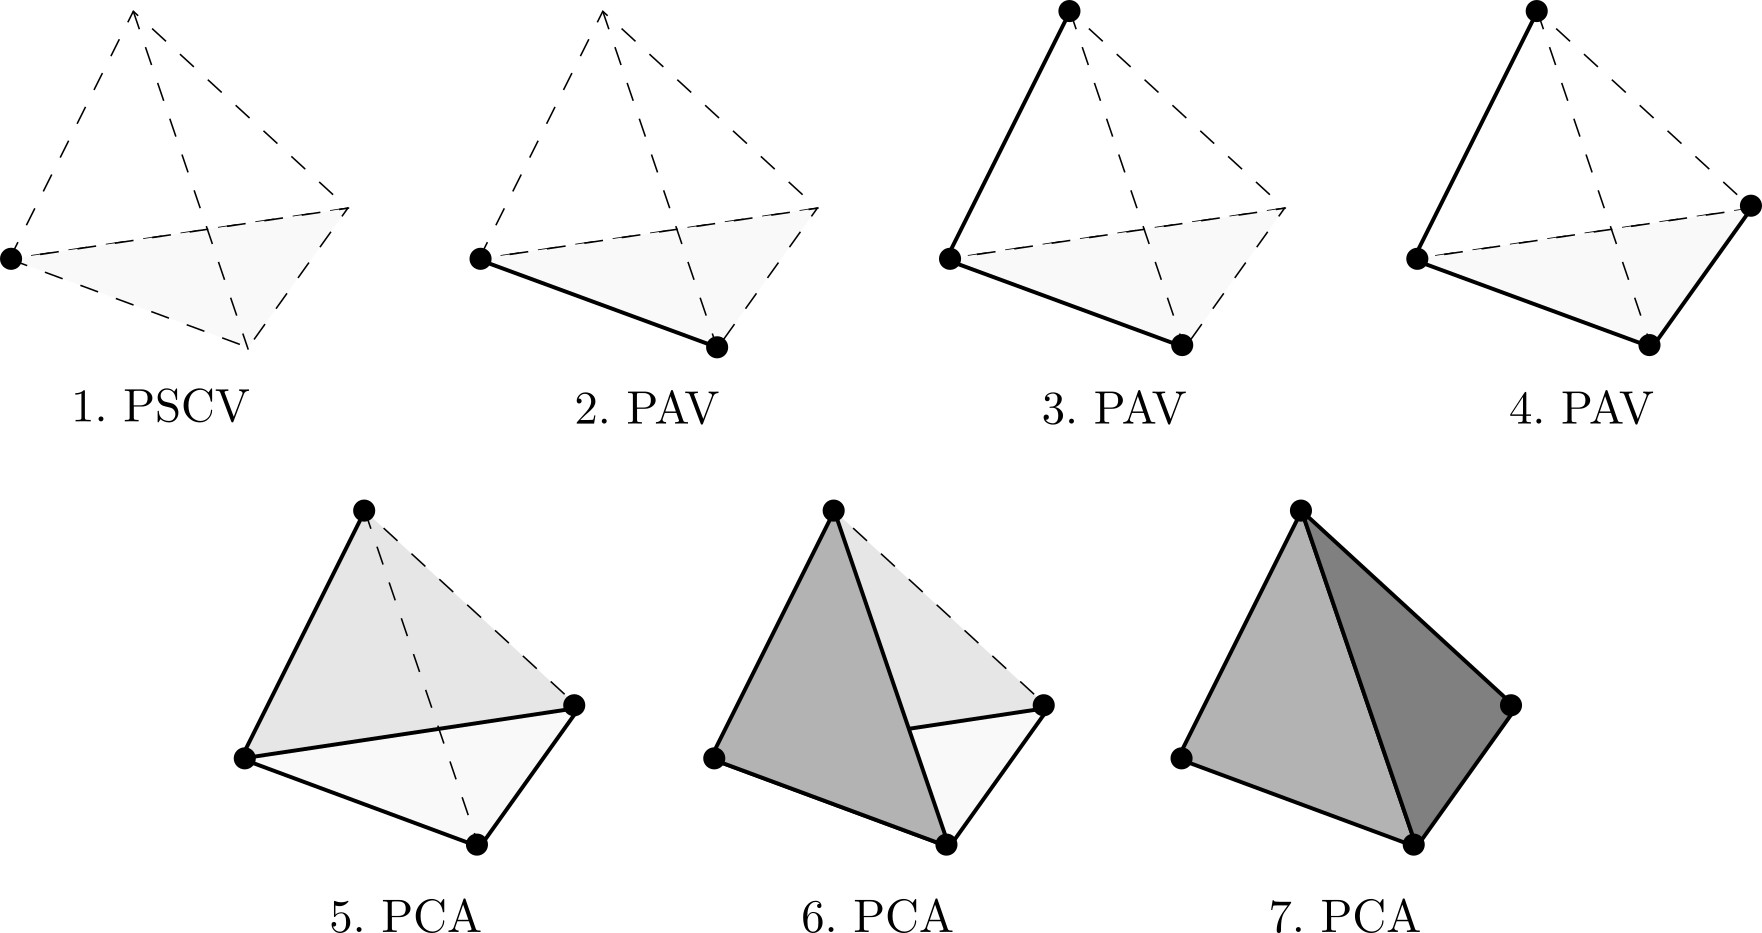
\includegraphics[width=12cm]{Img/GEO/geo-euler5.jpg}
\centering
\caption{\textbf{Figura 3.11. \footnotesize{Construcción de un tetraedro mediante los operadores de Euler.}}}
\end{figure}

Vemos en el ejemplo que la fórmula de Euler está equilibrada en todo momento, aunque no se obtiene un sólido válido hasta después de haber realizado la última operación. El primer operador (el PSCV) se encarga de inicializar la estructura de datos, y añade un vértice, una cara e incrementa el contador de superficies. Como argumentos requiere las coordenadas del vértice y los parámetros que describen la cara (no sus aristas).




\subsubsection{ Concepto de Frontera. }

Si se tiene una región n-dimensional $R^n$ en un espacio n-dimensional $E^n$, sus puntos pueden ser clasificados como: los que están dentro de la región y
los que están en su límite o frontera. Por lo tanto, el conjunto de puntos de $R^n$ estará formado por el subconjunto de puntos interior $(iR)$, más el conjunto de los puntos de la frontera $(fR)$.

$$R = [iR, fR]$$

Según lo anterior, cualquier punto en el espacio $E^n$, tiene la siguiente propiedad respecto a $R^n$:

\begin{itemize}
\item Pertenecer al interior de $R^n$, es decir a $iR$. 
\item Pertenecer a la frontera de $R^n$, es decir a $fR$.
\item No pertenecer a $R^n$. 
\end{itemize}


\begin{figure}[h]
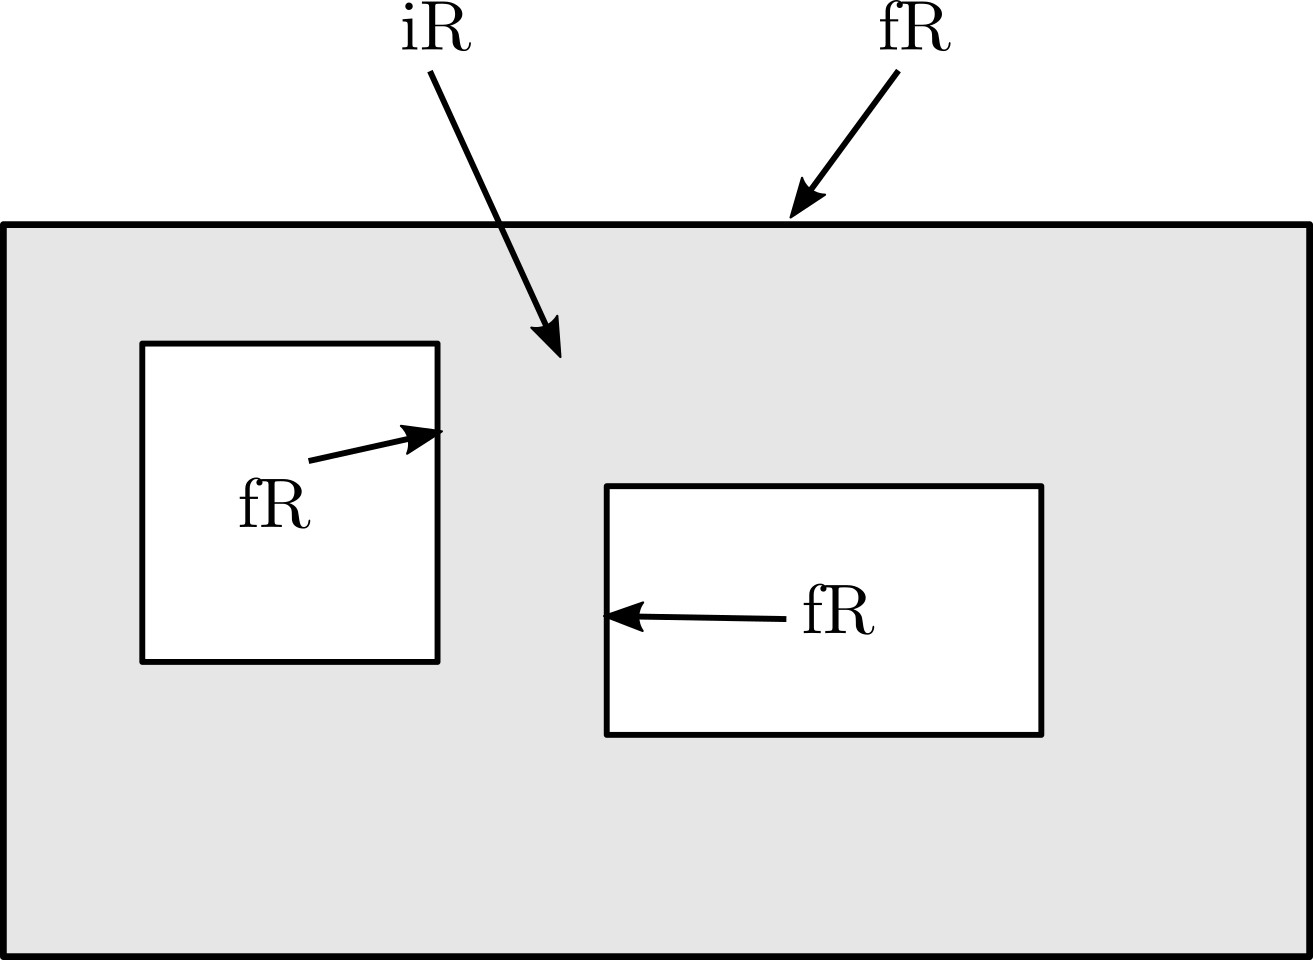
\includegraphics[width=8cm]{Img/GEO/geo-frontera0.jpg}
\centering
\caption{\textbf{Figura 3.11. \footnotesize{objetos planos con sus puntos frontera e interiores.}}}
\end{figure}

\subsubsection{ Operadores Booleanos. }

Los objetos geométricos pueden considerarse como conjuntos de puntos, tanto de interior como de frontera. En Modelado Sólido, para construir objetos complejos se utilizan operaciones entre conjuntos, tales como unión $(\cup)$, intersección $(\cap)$ y diferencia $(−)$. A estos operadores se les conoce en modelado como \textbf{operadores Booleanos}. Al aplicar los operadores booleanos sobre objetos simples para formar modelos más complejos, es importante que los modelos obtenidos sean íntegros (topológicamente válidos), y que además sean \textit{dimensionalmente homogéneos}, es decir, que su dimensión sea igual a la de los objetos que se combinan. La figura 25 muestra dos ejemplos donde se pierde la homogeneidad dimensional, después de efectuar la intersección entre objetos válidos de 2 y 3 dimensiones.


\begin{figure}[h]
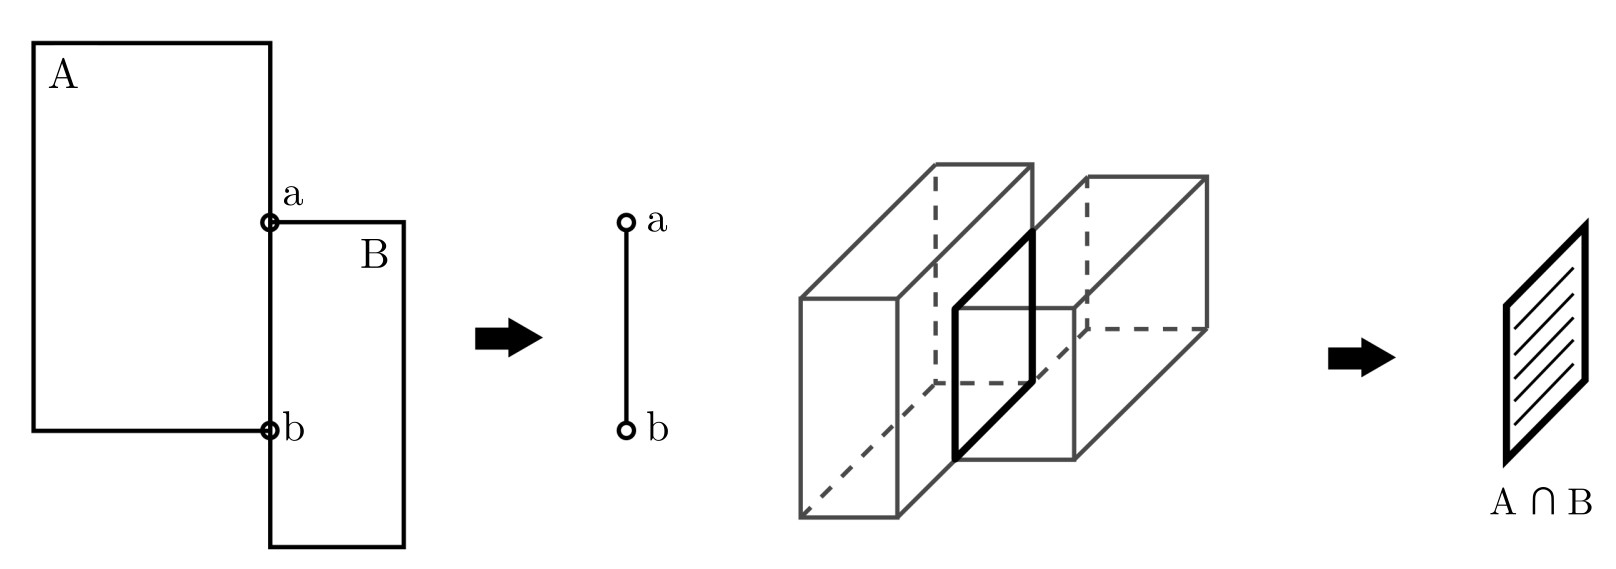
\includegraphics[width=14cm]{Img/GEO/geo-booleano0.jpg}
\centering
\caption{\textbf{Figura 3.11. \footnotesize{Intersección que presenta un resultado degenerado.}}}
\end{figure}

lndependientemente de cómo representemos los objetos, es necesario combinarlos para formar nuevos. Uno de los métodos más intuitivos y comunes para combinar objetos son las \textit{operaciones booleanas de conjuntos}, como la unión, la diferencia y la intersección, ilustradas en la figura 3.17.

\begin{figure}[h]
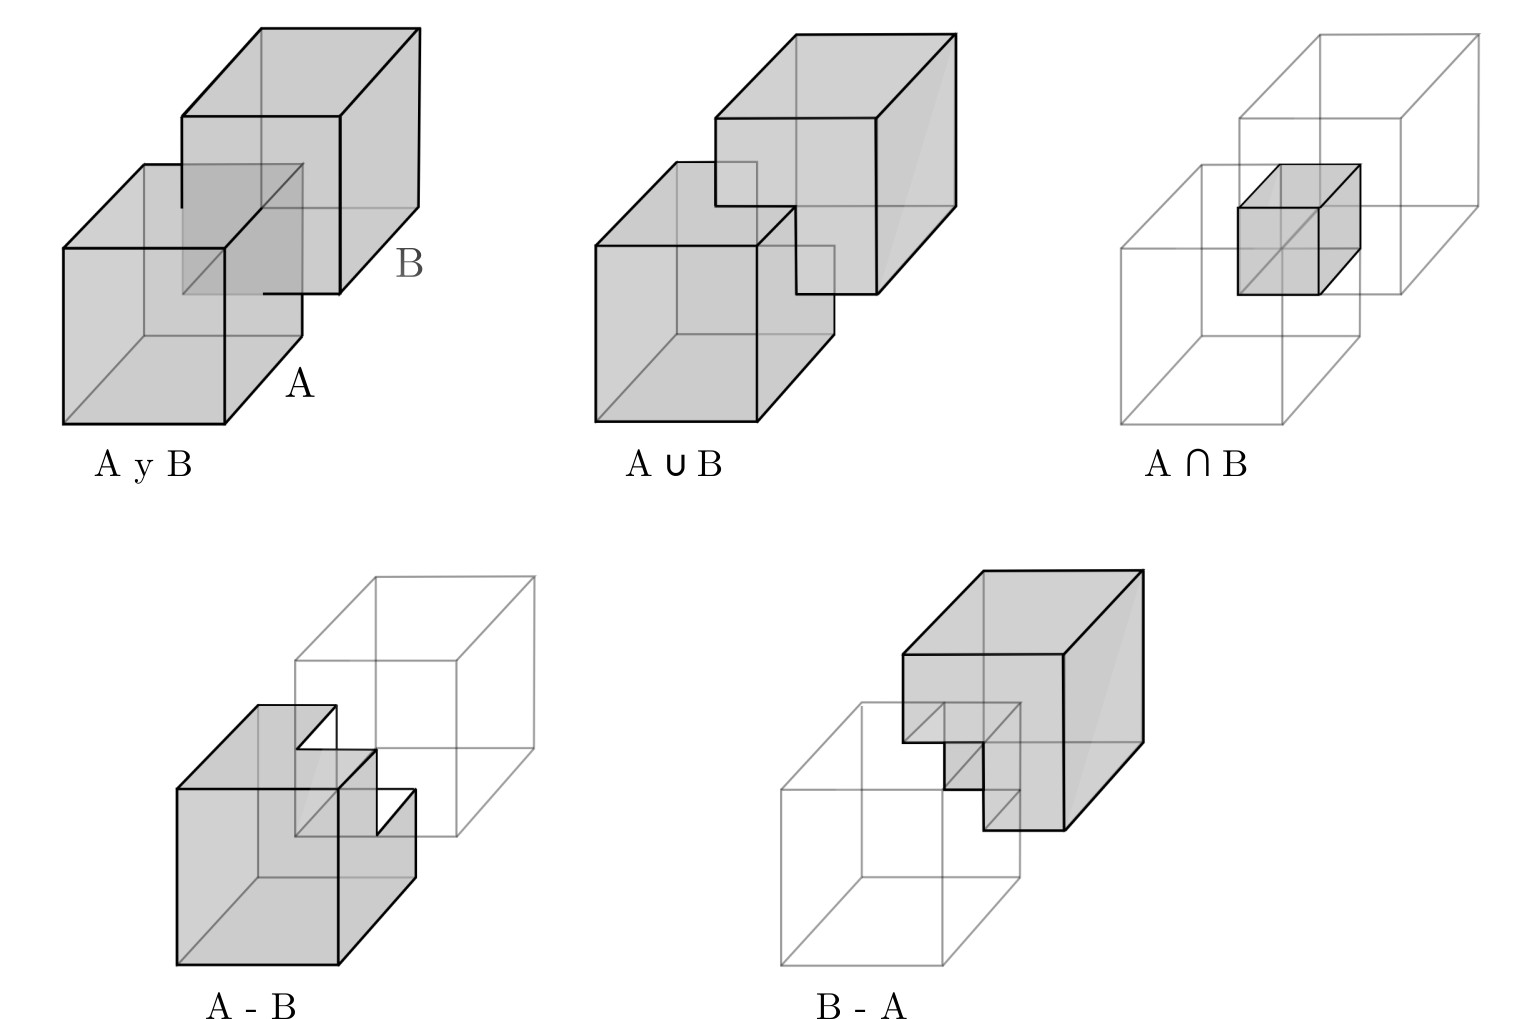
\includegraphics[width=14cm]{Img/GEO/geo-booleano1.jpg}
\centering
\caption{\textbf{Figura 3.11. \footnotesize{Operaciones booleanas Objetos $A y B$, $A \cup B$, $A \cap B$, $A - B$, $B - A$}}}
\end{figure}

\textbf{ Operadores booleanos regularizados }

La aplicación de una operación booleana ordinaria de conjuntos a dos objetos sólidos no necesariamente produce un objeto sólido. Por ejemplo, la intersección ordinaria de dos cubos que se unen en un solo vértice es un punto.\vskip
Para evitar los resultados degenerados se utiliza el conjunto de los \textbf{operadores regularizados}, que preservan la homogeneidad dimensional. Los operadores regularizados se denotan por $\cup^*$, $\cap^*$ y $-^*$ y se definen de manera que las operaciones con sólidos siempre generen sólidos.

\textbf{ A) Intersección Regularizada ($\cap^{*}$)}

\begin{figure}[h]
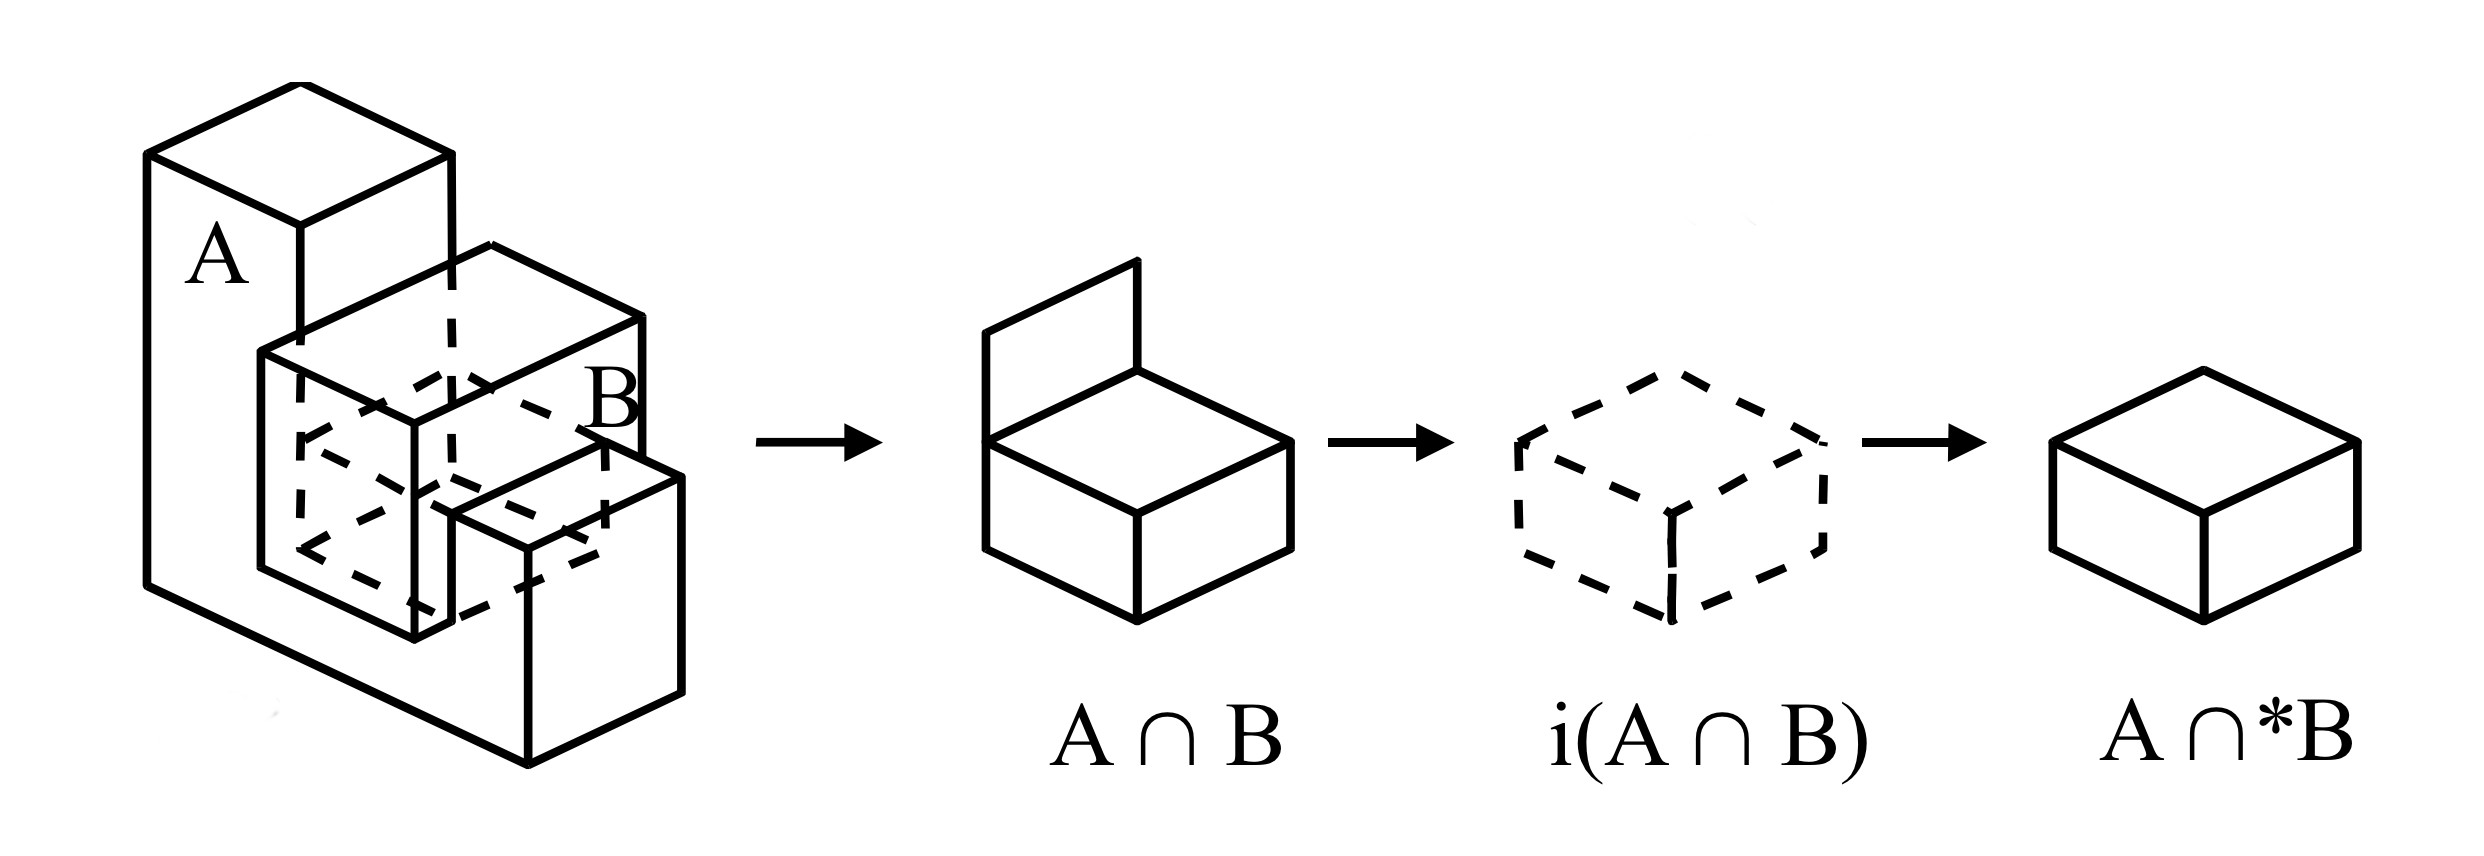
\includegraphics[width=12cm]{Img/GEO/geo-booleano2.jpg}
\centering
\caption{\textbf{Figura 3.11. \footnotesize{Intersección no regularizada ($\cap$) y regularizada ($\cap^*$) de dos solidos.}}}
\end{figure}

Para comprender el proceso de regularización se analizan los objetos bidimensionales A y B de la figura 26, si realizamos la intersección no regularizada $(\cap)$ con dichos objetos, se obtiene un objeto que no es dimensionalmente homogéneo en su totalidad, pues contiene una ``arista colgante". El resultado deseado se obtiene mediante la intersección regularizada $(\cap^*)$ de A y B.


\begin{figure}[h]
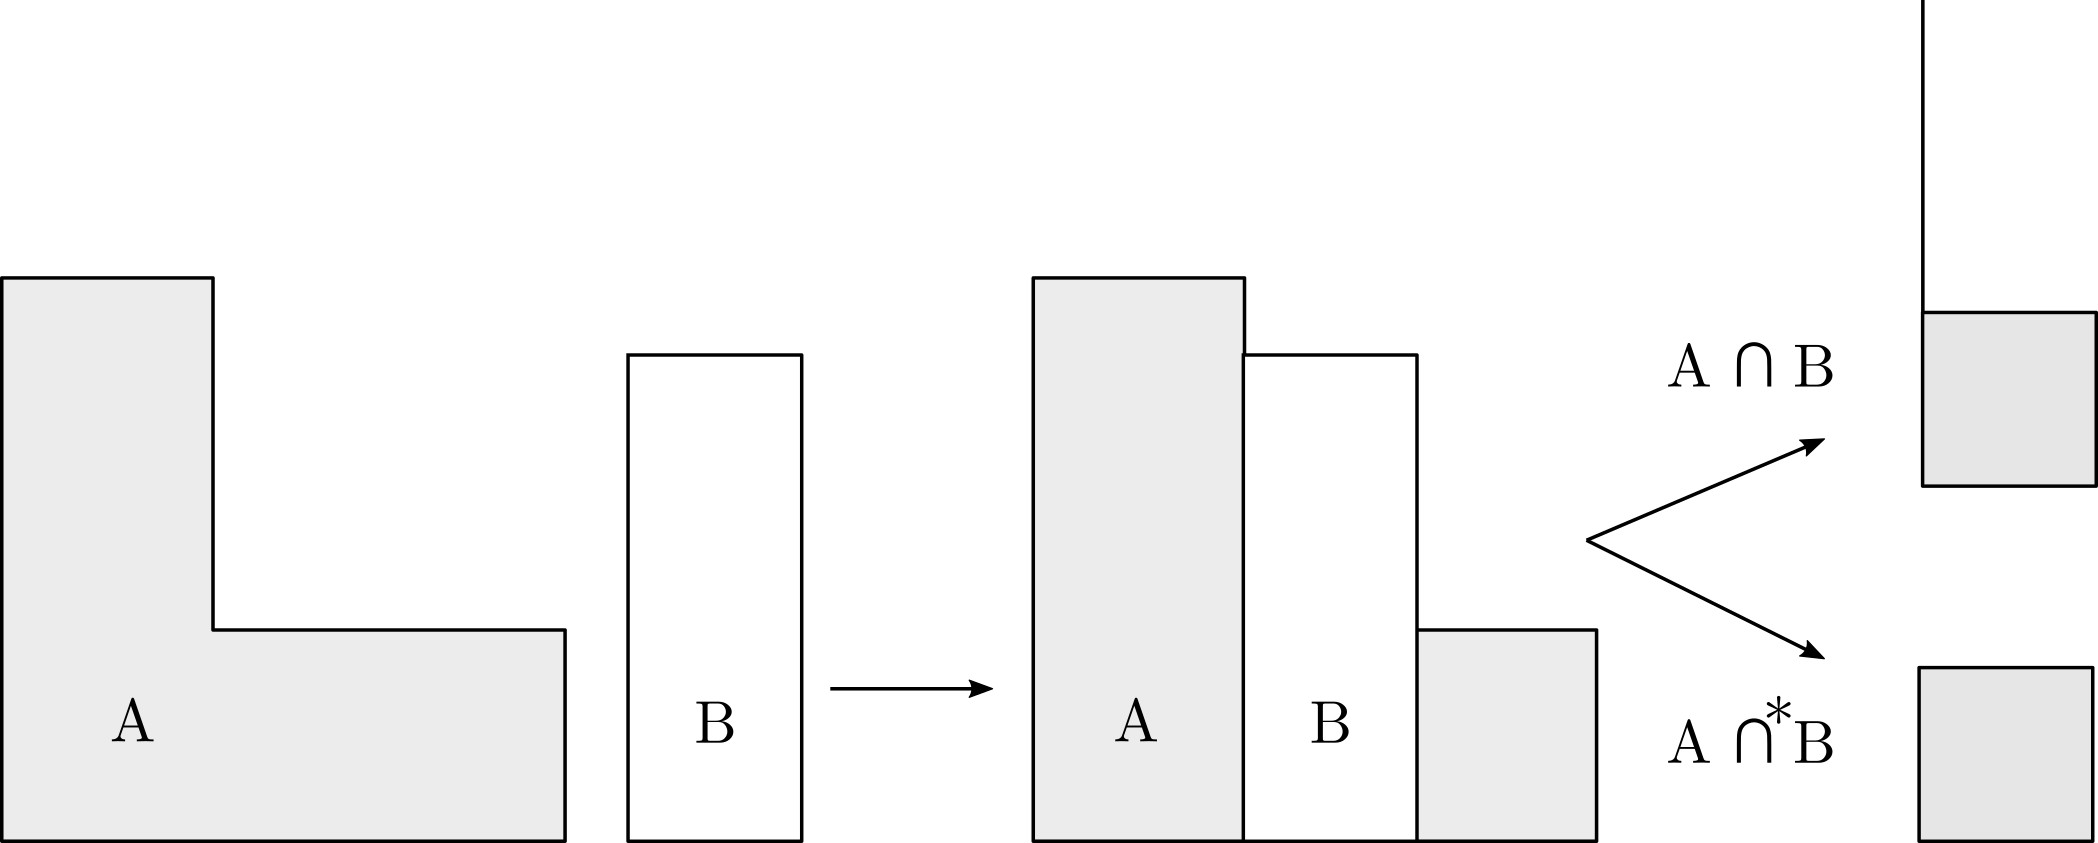
\includegraphics[width=12cm]{Img/GEO/geo-booleano3.jpg}
\centering
\caption{\textbf{Figura 3.11. \footnotesize{operador booleano de intersección no regularizado $(\cap)$ y el regularizado $(\cap^*)$.}}}
\end{figure}




Los objetos A y B se pueden representar como la unión de los subconjuntos de frontera e interior. Así:

\begin{center}
   $A = iA \cup fA$ y $B = iB \cup fB$
\end{center}

Por tanto, es posible expresar la intersección no regularizada de A y B como:

$$C = A \cap B = (iA \cup fA) I (iB \cup fB)$$ 

Aplicando la propiedad distributiva queda:

$$C = (iA \cap iB) \cup (iA \cap fB) \cup (fA \cap iB) \cup (fA \cap fB)$$

En la figura 27 podemos ver la representación gráfica de cada uno de los términos de la expresión anterior.

\begin{figure}[h]
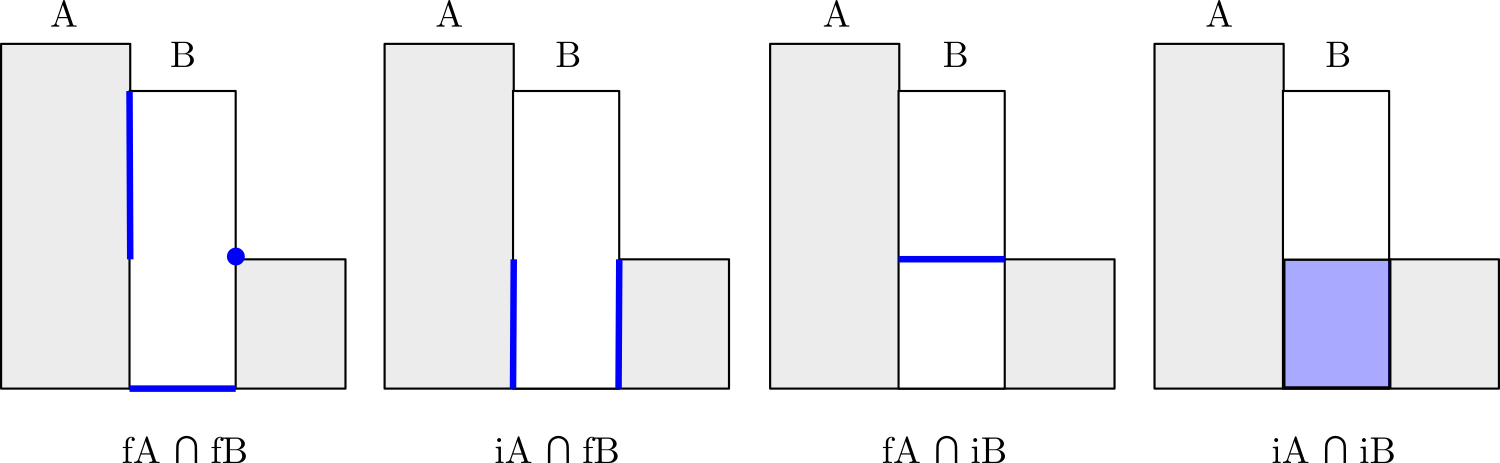
\includegraphics[width=14cm]{Img/GEO/geo-booleano4.png}
\centering
\caption{\textbf{Figura 3.11. \footnotesize{subconjuntos de puntos al efectuar $A \cap B$.}}}
\end{figure}

En principio, cada uno de los términos de la Ec. 21 es candidato para formar parte del resultado regularizado (homogéneo dimensional), al que llamaremos \textbf{$C^*$}. 
Dado que $C^*$ se trata de un conjunto de puntos, de nuevo se tiene que:

$$C^* = iC^* \cup fC^*$$

En la figura 27 se puede ver que $iC = iC^* = iA \cap iB$. Queda entonces por determinar $fC^*$, que será igual a la parte válida de ($fA \cap fB$).\vskip
Ver que las fronteras de los nuevos elementos siempre consistirán en segmentos de fronteras de los elementos que se combinan. Se puede generalizar esta observación diciendo: \textit{los puntos de frontera pueden llegar a ser puntos de interior, mientras que los puntos de interior nunca pueden llegar a ser puntos de frontera}.\vskip
Además, en las intersecciones regularizadas, aunque no se incluya la demostración, ocurre que:
$$iA \cup fB \subset fC^* $$
$$fA \cup iB \subset fC^* $$

Por tanto, tres de los términos de la Ec. 21 son validos para formar fC*.
Sólo queda por analizar el candidato ($fA \cap fB$). Éste término es el único que puede dar problemas de homogeneidad dimensional, ya que pueden surgir subconjuntos de dimensión menor.\vskip
Entre los conjuntos de puntos que se forman al hacer ($fA \cap fB$) (fig. 27, izq.), el punto aislado es un candidato válido de $C^*$ ya que siempre será un vértice o cruce entre dos fronteras.
En cuanto a los restantes subconjuntos (segmentos en el ejemplo), para determinar cuáles pertenecen a $fC^*$, se aplica una \textit{prueba de pertenencia} como la siguiente:

\begin{enumerate}
\item Se establece para los dos objetos A y B un mismo sentido de giro, p. e., el sentido de giro contrario al de las agujas del reloj.
\item Para cada segmento de ($fA \cap fB$) se elige un punto $``P_0"$ del segmento.
\item Se traza un vector partiendo de $``P_0"$, en el sentido de giro de A, y otro en el sentido de giro de B.
\item Si los vectores tienen sentidos opuestos, el segmento no es válido. En caso contrario el segmento pertenece a $fC^*$.
\end{enumerate}

La figura 28 muestra gráficamente el test anterior

\begin{figure}[h]
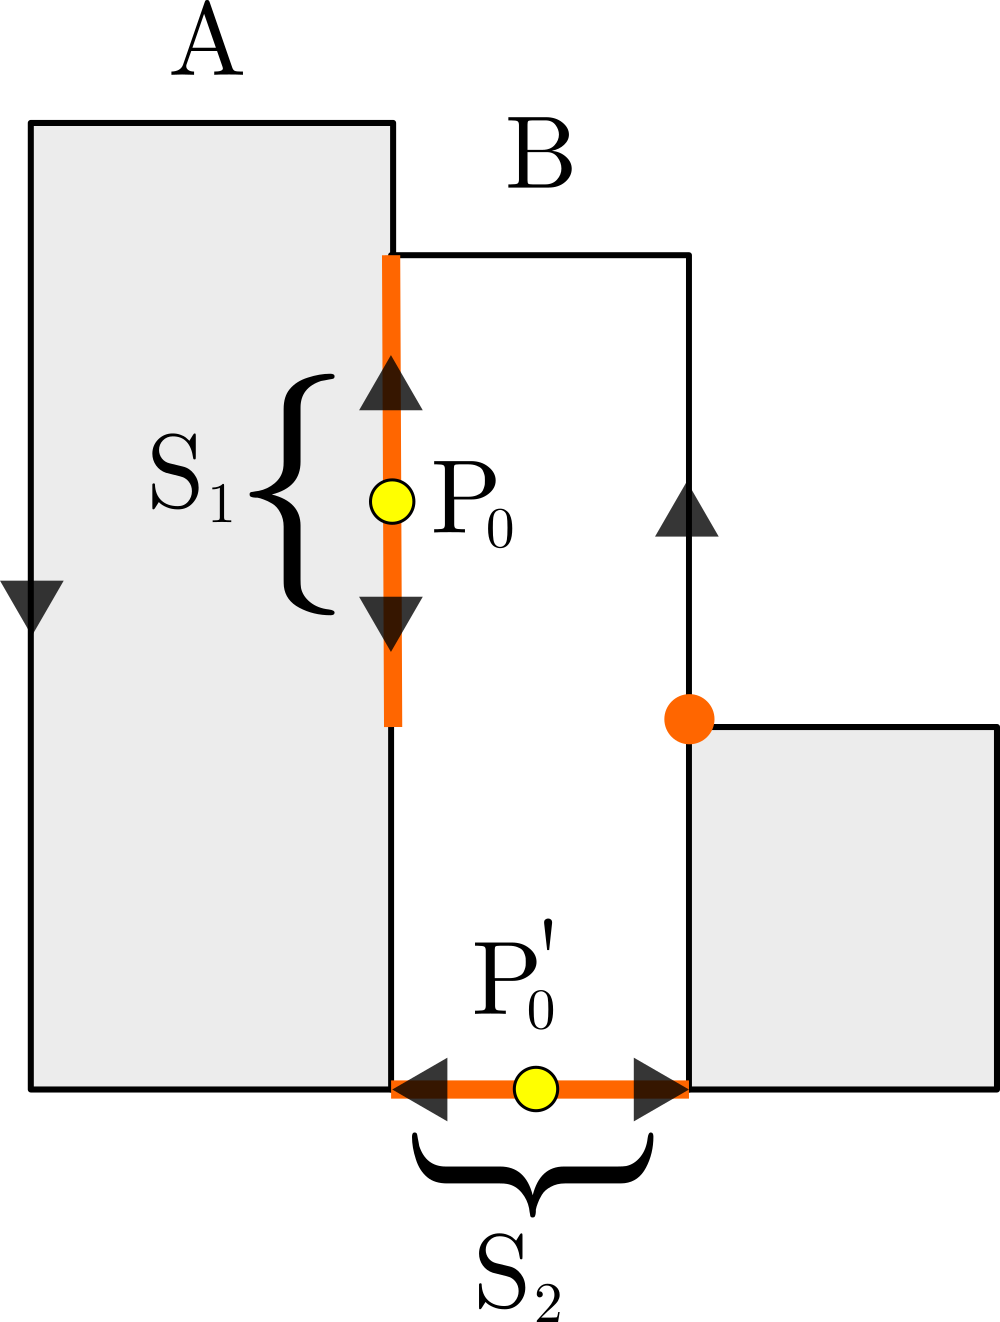
\includegraphics[width=4cm]{Img/GEO/geo-booleano5.png}
\centering
\caption{\textbf{Figura 3.11. \footnotesize{test de validación de un conjunto de puntos de frontera.}}}
\end{figure}

Aplicando esta prueba de validez, el segmento $S_1$ queda eliminado de $fC^*$, mientras que $S_2$ queda admitido. Resumiendo, hemos visto que haciendo
$$C^* (A \cap^* B) = válidos(iA \cap iB) \cup (iA \cap fB) \cup (fA \cap iB) \cup (fA \cap fB)$$

se obtiene la intersección regularizada de los objetos A y B, que mantiene la homogeneidad dimensional, respecto de A y B.\vskip
Para desarrollar los operadores booleanos restantes se procede de modo similar, es decir, se dividen los objetos de partida en subconjuntos interior y frontera y se realiza la operación booleana entre dichos subconjuntos, produciéndose candidatos para formar parte de $C^*$. (ver [Mort85], pgs. 408-413).

\subsubsection{ Clasificación de los elementos de un conjunto. }

Para regularizar los resultados booleanos es preciso determinar si los puntos se encuentran en el interior, la frontera o fuera de los conjuntos resultantes.
Se entiende por \textit{clasificación de los elementos de un conjunto}, a la inclusión de los miembros de ese conjunto en uno de estos subconjuntos:
\begin{itemize}
\item \textit{Conjunto de los puntos interiores (iA)}.
\item \textit{Conjunto de los puntos de la frontera (fA)}.
\item \textit{Conjunto de los puntos externos (cA)}.
\end{itemize}

Además de la regularización de los resultados, en Modelado Sólido es interesante realizar una clasificación de los elementos de un conjunto, para determinar las relaciones de inclusión entre los elementos geométricos, como por ejemplo:
\begin{itemize}
\item dados un sólido y un punto, determinar si el punto está dentro, fuera o en la frontera del sólido.
\item dados un polígono y una línea, determinar qué parte de la línea está dentro, qué parte fuera, y qué parte está en la frontera del polígono.
\item dados dos sólidos, determinar cuándo se tocan (problema típico de animación).
\item dados dos polígonos, determinar cuál es su intersección.
\end{itemize}


\textbf{ Criterios de clasificación en espacios n-dimensionales }\vskip
Para estudiar este tipo de problemas se establecen unos criterios de clasificación generales, organizados según la dimensión del espacio donde se definen.\vskip
En $E0$ la relación básica es entre dos puntos. Éstos pueden coincidir o pueden ser distintos; en este segundo caso, pueden estar lejos o cerca.\vskip
En $E1$, dada una curva, hay varias clasificaciones posibles. Un punto puede ser el punto inicial, el punto final, o un punto intermedio de la curva. En una línea recta pueden darse otras dos clasificaciones: un punto puede estar delante o detrás de la línea, en la misma dirección. Por último, otras clasificaciones posibles son: un punto puede estar a la derecha de la línea o a su izquierda.\vskip
En $E2$, si se trata de un disco topológico, se puede averiguar si un punto está dentro, fuera o en la frontera del disco topológico.\vskip
Finalmente, en $E3$, dado un sólido, un punto puede estar dentro, en la superficie o fuera. Si el sólido es un poliedro, y si el punto está en la superficie, podría encontrarse en una cara, en una arista o en un vértice.
Estas son, más o menos, las posibles clasificaciones que pueden hacerse de los elementos de $E0$, con respecto a $E1$, $E2$ y $E3$.\vskip
En modelado, tan importante como la clasificación de los puntos es la clasificación de los elementos de $E1$ (líneas y curvas) en $E1$, $E2$ y $E3$. Es muy común el tener que averiguar la intersección entre líneas, la intersección y recorte (clipping) entre líneas y polígonos y la intersección entre líneas y sólidos (p. e. en ray tracing).\vskip
No menos importante es la clasificación entre los elementos de $E2$ (planos, polígonos y superficies curvas) en $E2$ y $E3$, es decir, localizar las intersecciones de superficies (que como veremos será muy importante a la hora de fronterizar los modelos booleanos) y los cortes entre planos y/o superficies y los sólidos.
Finalmente, la clasificación de los elementos de $E3$ con los de $E3$ también es importante, especialmente en animación y modelado, para la detección de colisiones entre los objetos y la composición de modelos complejos, a partir de otros más simples.

\subsubsection{Representaciones de barrido}
Al barrer un objeto a lo largo de una trayectoria por el espacio se define un objeto nuevo, llamado barrido. El barrido más sencillo es el definido por un área bidimensional barrida por una trayectoria lineal normal al plano del área para crear un volumen. Este proceso se conoce como barrido traslacional o \textbf{extrusión} y es una forma natural de representar objetos formados por la extrusión de metal o plástico a través de un molde con la sección transversal deseada.\vskip
En los casos más sencillos cada volumen de barrido no es más que el área del objeto que se barre multiplicada por la longitud del barrido. Las extensiones sencillas comprenden el escalamiento de la sección transversal durante el barrido para producir un objeto ahusado o barrer la sección transversal a lo largo de una trayectoria lineal que no es la normal. Los barridos rotacionales se definen mediante la rotación de un área con respecto a un eje.\vskip
El objeto que se barre no tiene que ser bidimensional. Los barridos de sólidos son útiles para modelar la región barrida por la cabeza de corte de una máquina herramienta o un robot que sigue una trayectoria. Los barridos donde el área o el volumen que generan cambia de tamaño, forma u orientación y que siguen una trayectoria curva arbitraria se denominan barridos generales.\vskip
Los \textit{barridos generales} de secciones transversales bidimensionales generalmente se modelan como secciones transversales bidimensionales parametrizadas barridas con ángulos rectos sobre una curva arbitraria. Los barridos generales son muy difíciles de modelar en forma eficiente. Por ejemplo, la trayectoria y la forma del objeto que producen pueden ocasionar que el objeto se interseque, complicando los cálculos de volumen. Además, los barridos generales no siempre generan sólidos. Por ejemplo, el barrido de un área bidimensional en su propio plano genera otra área bidimensional.\vskip
En términos generales, es difícil aplicar las operaciones regularizadas de conjuntos booleanos a los barridos sin antes convertirlos a otra representación. Incluso los barridos más simples no son cerrados con las operaciones booleanas regularizadas de conjuntos. Por ejemplo, al unión de dos barridos simples generalmente no es un barrido simple, como se ilustra en la figura 3.22.

\begin{figure}[h]
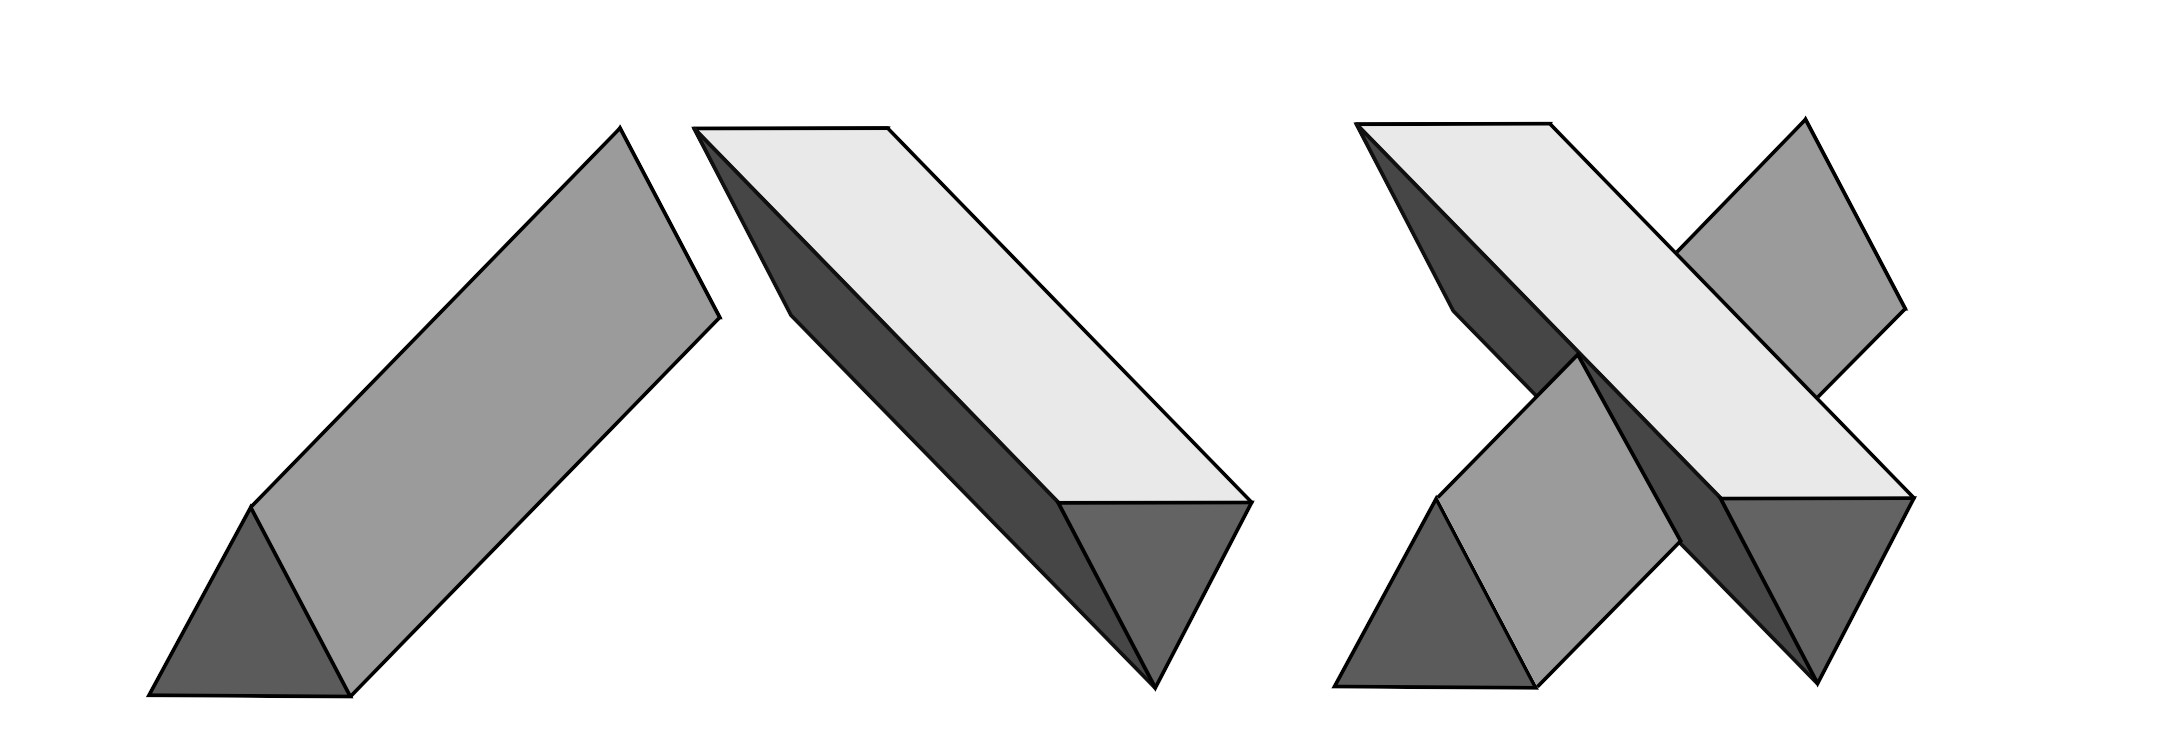
\includegraphics[width=8cm]{Img/GEO/geo-extrude.jpg}
\centering
\caption{\textbf{Figura 3.11. \footnotesize{3.22. Dos barridos traslacionales definidos por triángulos. La unión de los barridos representados no es un barrido simple de un objeto tridimensional.}}}
\end{figure}

Sin embargo, a pesar de los problemas de cerradura y de cálculo, los barridos son una
forma natural e intuitiva de construir diversos objetos. Por ello, muchos sistemas de modelado de sólidos permiten a los usuarios construir objetos como barridos, pero los almacenan con alguna representación.

\begin{figure}[h]
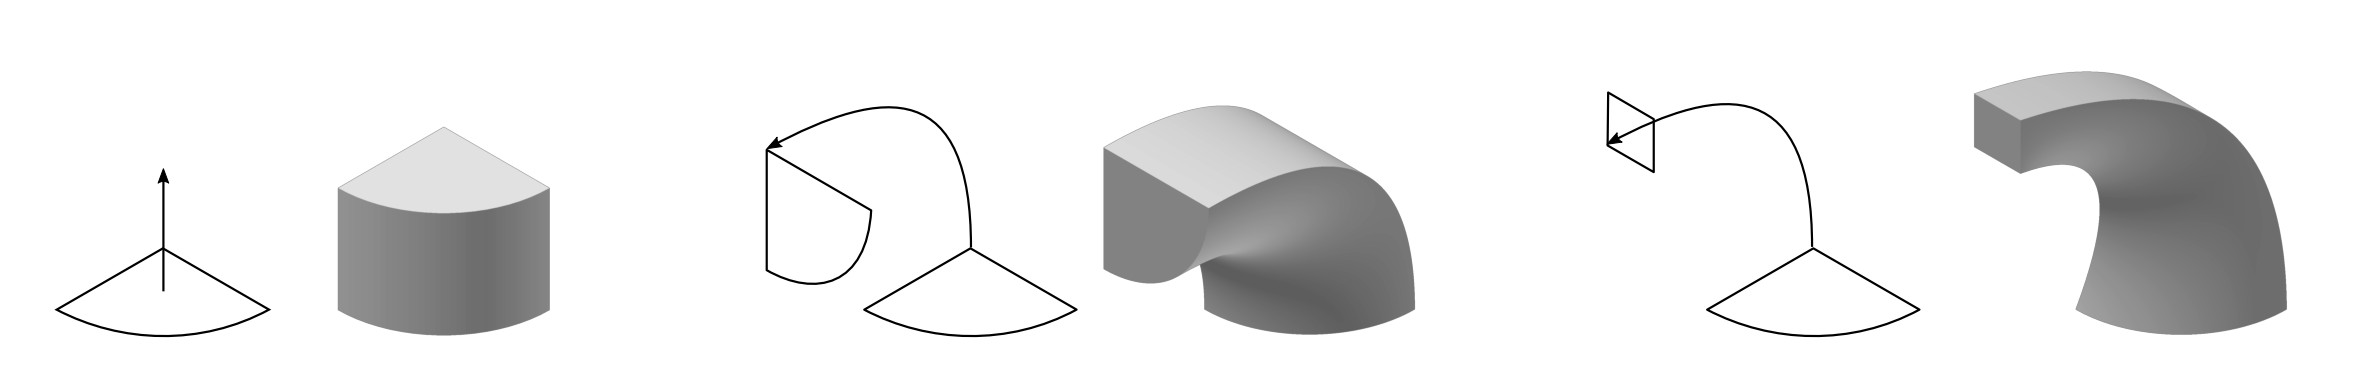
\includegraphics[width=16cm]{Img/GEO/geo-extrude1.jpg}
\centering
\caption{\textbf{Figura 3.11. \footnotesize{3.22.  Extrusión (barrido traslacional), Sweep(barrido general) y Loft(barrido general) respectivamente. }}}
\end{figure}

\subsection{ Problemas del Modelado Sólido }

El requerimiento de aplicabilidad general de los modelos sólidos implica la necesidad de que sean completos y exactos. Conseguir esto resulta problemático.
A continuación se explican los puntos más conflictivos: 

\subsubsection{Que sean completos}

En general, los modelos gráficos 2D no sirven para el Modelado Sólido, ya que no se puede responder algorítmicamente a todas las preguntas geométricas en tres dimensiones, a partir de los dibujos realizados en 2D.
Los modelos gráficos bidimensionales pueden ser transformados en modelos tridimensionales, añadiendo la información de la tercera coordenada.
De esta forma se obtiene una representación de sólidos conocida normalmente como modelo alámbrico \footnote{Los modelos alámbricos se caracterizan por no disponer de superficies, sólo consta de puntos, líneas y curvas con las que se describen los lados de los objetos.} del inglés \textit{wireframe model}. Con el modelo alámbrico es posible almacenar un solo modelo tridimensional, y generar todas las vistas bidimensionales a partir de él, superándose de esta manera los problemas planteados por los modelos gráficos en 2D.
Sin embargo, un grupo de líneas tridimensionales no es suficiente para representar una figura ya que, en ocasiones, se pueden dar varias interpretaciones.
Un ejemplo común es mostrado en la figura 2.

\begin{figure}[h]
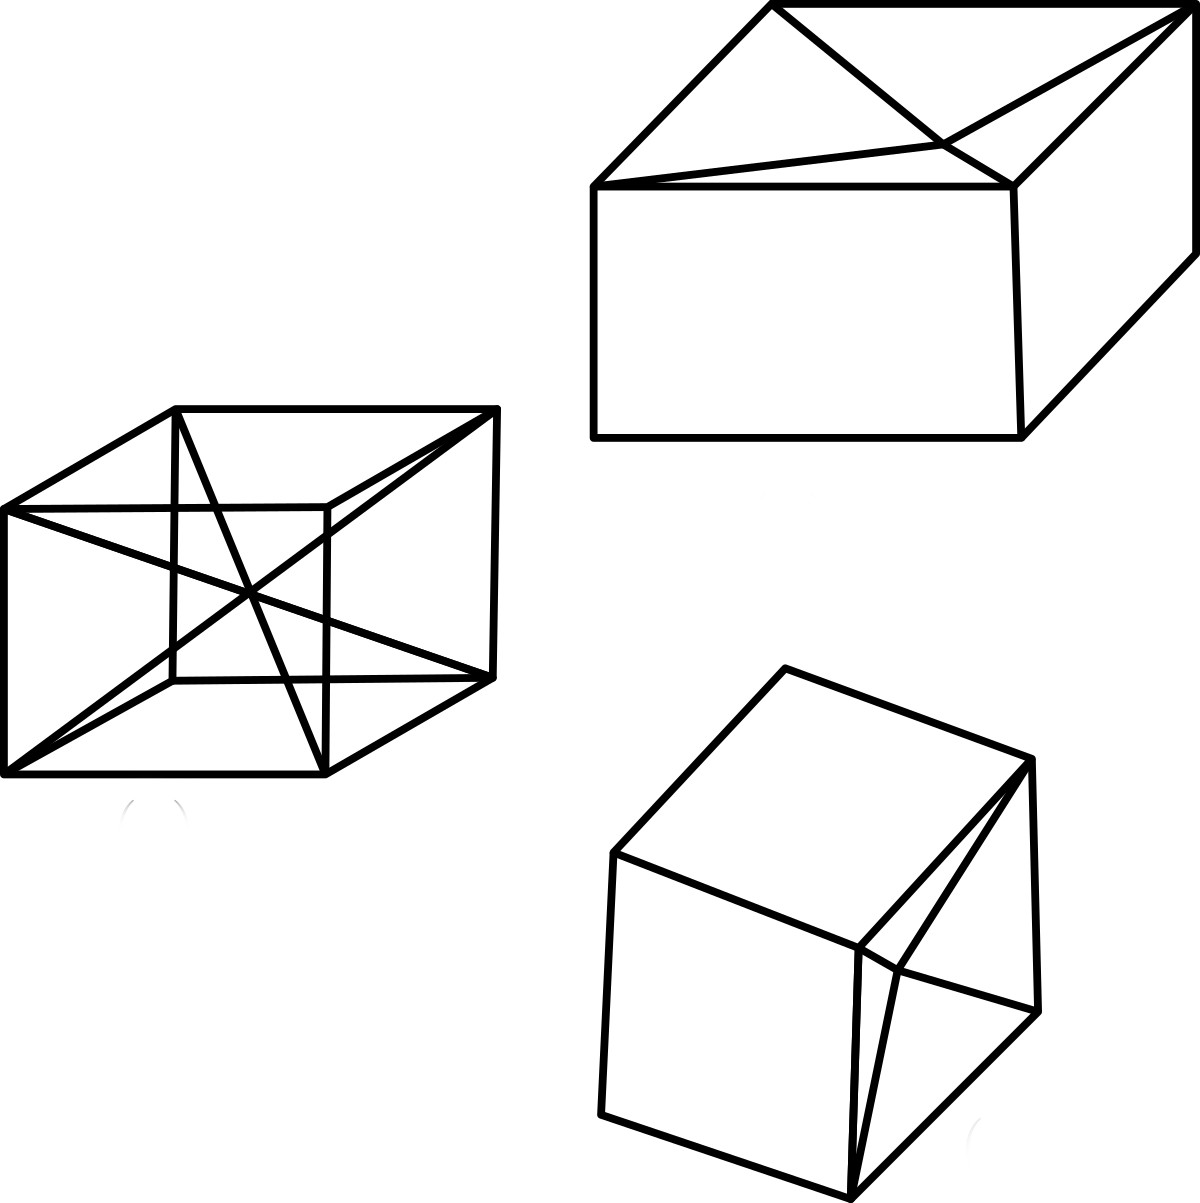
\includegraphics[width=6cm]{Img/GEO/geo-problema.jpg}
\centering
\caption{\textbf{Figura 3.11. \footnotesize{posibles interpretaciones de un modelo gráfico ambiguo. }}}
\end{figure}

\vskip
Otro problema que plantean los modelos alámbricos es que permiten el diseño de objetos que no pueden ser creados como objetos 3D reales, según se muestra en la figura 3 
\begin{figure}[h]
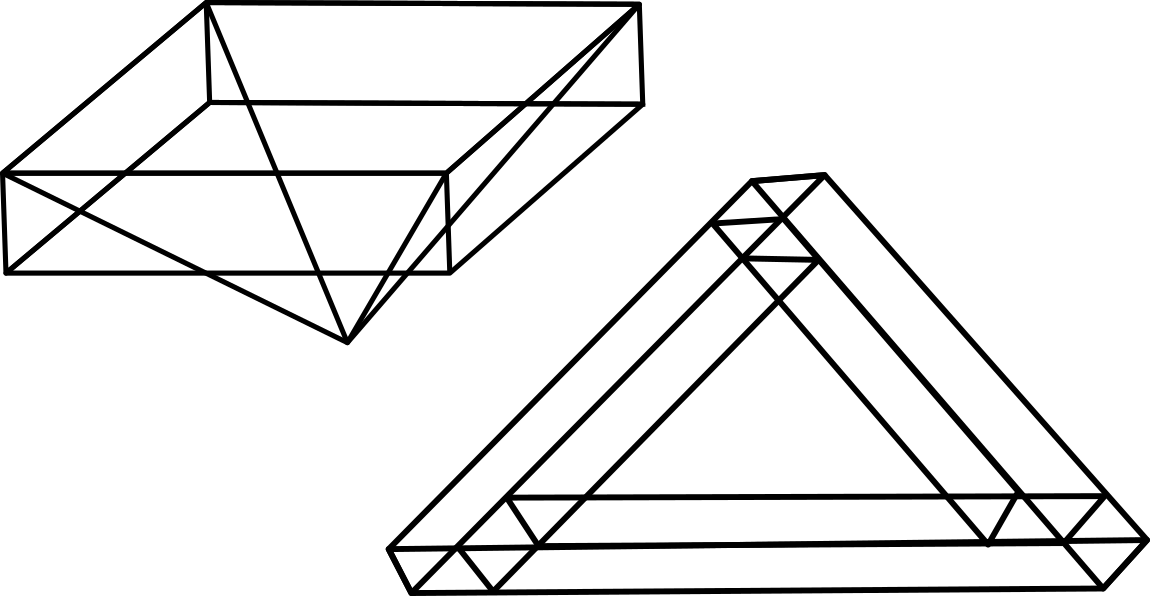
\includegraphics[width=10cm]{Img/GEO/geo-problema1.png}
\centering
\caption{\textbf{Figura 3.11. \footnotesize{posibles interpretaciones de un modelo gráfico ambiguo. }}}
\end{figure}

\vskip
Otra deficiencia de los modelos alámbricos es la falta de contorno o información de perfil para las superficies supuestas entre las aristas alámbricas.
(ver la figura 4)

\begin{figure}[h]
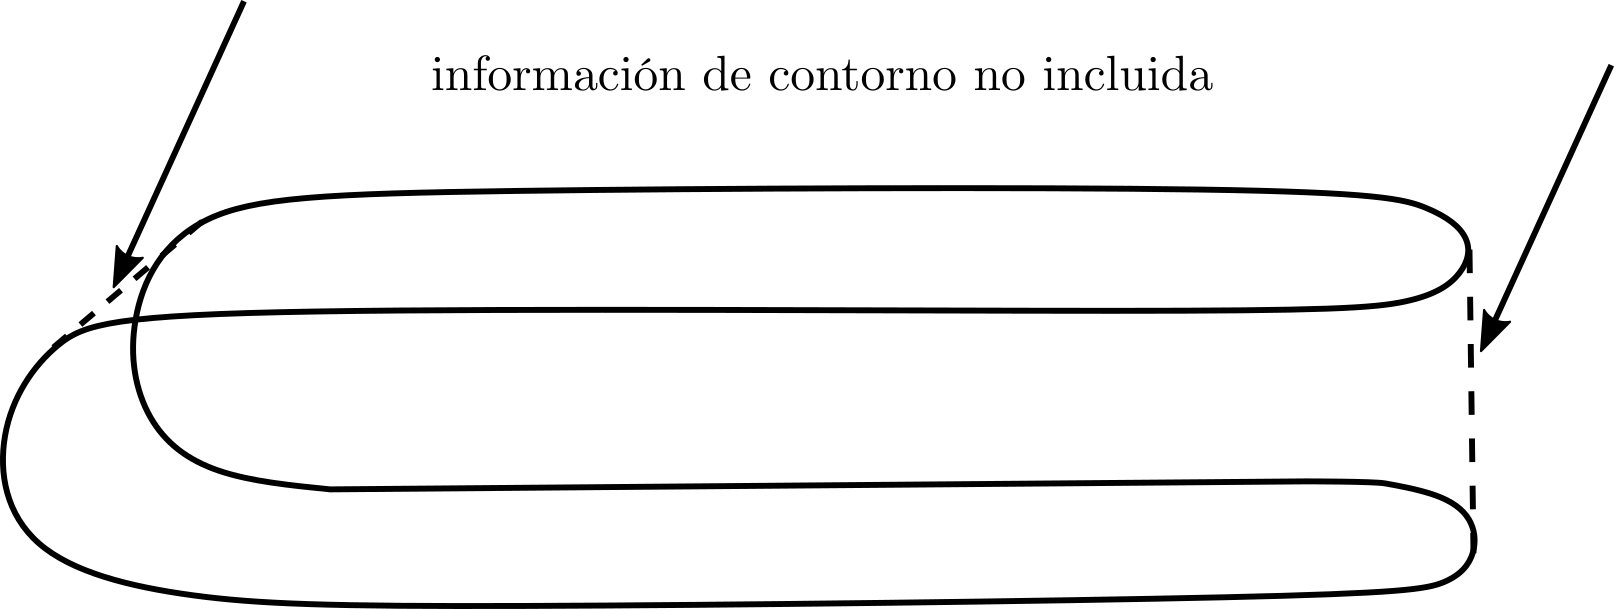
\includegraphics[width=12cm]{Img/GEO/geo-problema2.png}
\centering
\caption{\textbf{Figura 3.11. \footnotesize{información de contorno perdida. }}}
\end{figure}



\subsubsection {Integridad}

Para resolver el problema de eliminar líneas y superficies ocultas, normalmente
se reemplazan los modelos gráficos por \textit{modelos poliédricos}\footnote{Un modelo poliédrico es un modelo geométrico cuyas caras son planas y encierran un volumen finito.} Estos modelos proporcionan la suficiente información para identificar las partes de los objetos que quedan ocultas al observador. Se construyen a partir de primitivas bidimensionales (polígonos) en vez de sólo líneas.\vskip
Al remplazar líneas por polígonos aparecen nuevos problemas. Normalmente,los algoritmos de eliminación de líneas ocultas asumen que los polígonos no intersectan entre sí, excepto en los vértices y aristas comunes.
Obviamente, un modelo poliédrico no puede incluir polígonos con intersecciones entre ellos, pues la superficie del objeto tendría intersecciones consigo misma. Por lo tanto, sólo se considerarán válidos a aquellos modelos poliédricos con polígonos sin intersecciones mutuas. Pero ¿cómo asegurarse de que los modelos cumplen este criterio?\vskip
El comprobar que el Modelado Sólido cumple este u otros requisitos preserva la \textit{integridad} del modelo, evitando la generación de modelos incorrectos.
Sin embargo, la comprobación de la integridad de los modelos trae consigo una disminución en la facilidad de uso y flexibilidad de los sistemas de modelado. 

\subsubsection{Complejidad y cobertura geométrica} El problema de la integridad está relacionado con otro: la \textit{complejidad} en la generación de un modelo poliédrico. Incluso objetos relativamente simples requieren más de cien polígonos; generar toda esa información a mano es complicado, tedioso y propenso a errores.
La \textit{cobertura geométrica} de un modelo poliédrico no es suficiente para tareas que requieren un modelado exacto de superficies curvas (como la carrocería de un coche), motivo por el cual se han desarrollado métodos para manejar formas complejas. 


\subsection{ Modelado Booleano (CSG) }

Al conjunto de procesos que permiten el diseño de sólidos complejos mediante la combinación booleana de objetos simples (primitivas) se conoce como modelado booleano, o también como Geometría Constructiva de Sólidos en inglés \textit{Constructive Solid Geometry} (CSG).\vskip
En el modelado booleano, después de trasladar, girar y escalar convenientemente las primitivas, se aplican los operadores booleanos regularizados ($\cup^*$, $\cap^*$ y $-^*$) para combinarlas. Además de los procesos anteriores, también son necesarios métodos de clasificación de vértices y aristas, así como de evaluación de fronteras.
Dado que los operadores booleanos son regularizados, todos los sólidos con los que se va a operar, así como los objetos resultantes, han de tener la misma dimensión espacial.\vskip
Un sólido construido mediante un modelador booleano queda descrito mediante un árbol binario en el que:

\begin{itemize}
\item El nodo raíz es el sólido resultante.
\item Los nodos internos son los operadores booleanos.
\item Los nodos hoja son las primitivas.
\end{itemize}

En los nodos terminales del árbol no sólo se representan las primitivas, sino que también se indican las transformaciones lineales que se han de efectuar sobre ellas. En el árbol, tanto las operaciones como los nodos hoja deberán encontrarse ordenadas, debido a que las operaciones booleanas no son, en general, conmutativas. El proceso de seguimiento (recorrido) del árbol se hará partiendo de los nodos terminales.

\begin{figure}[h]
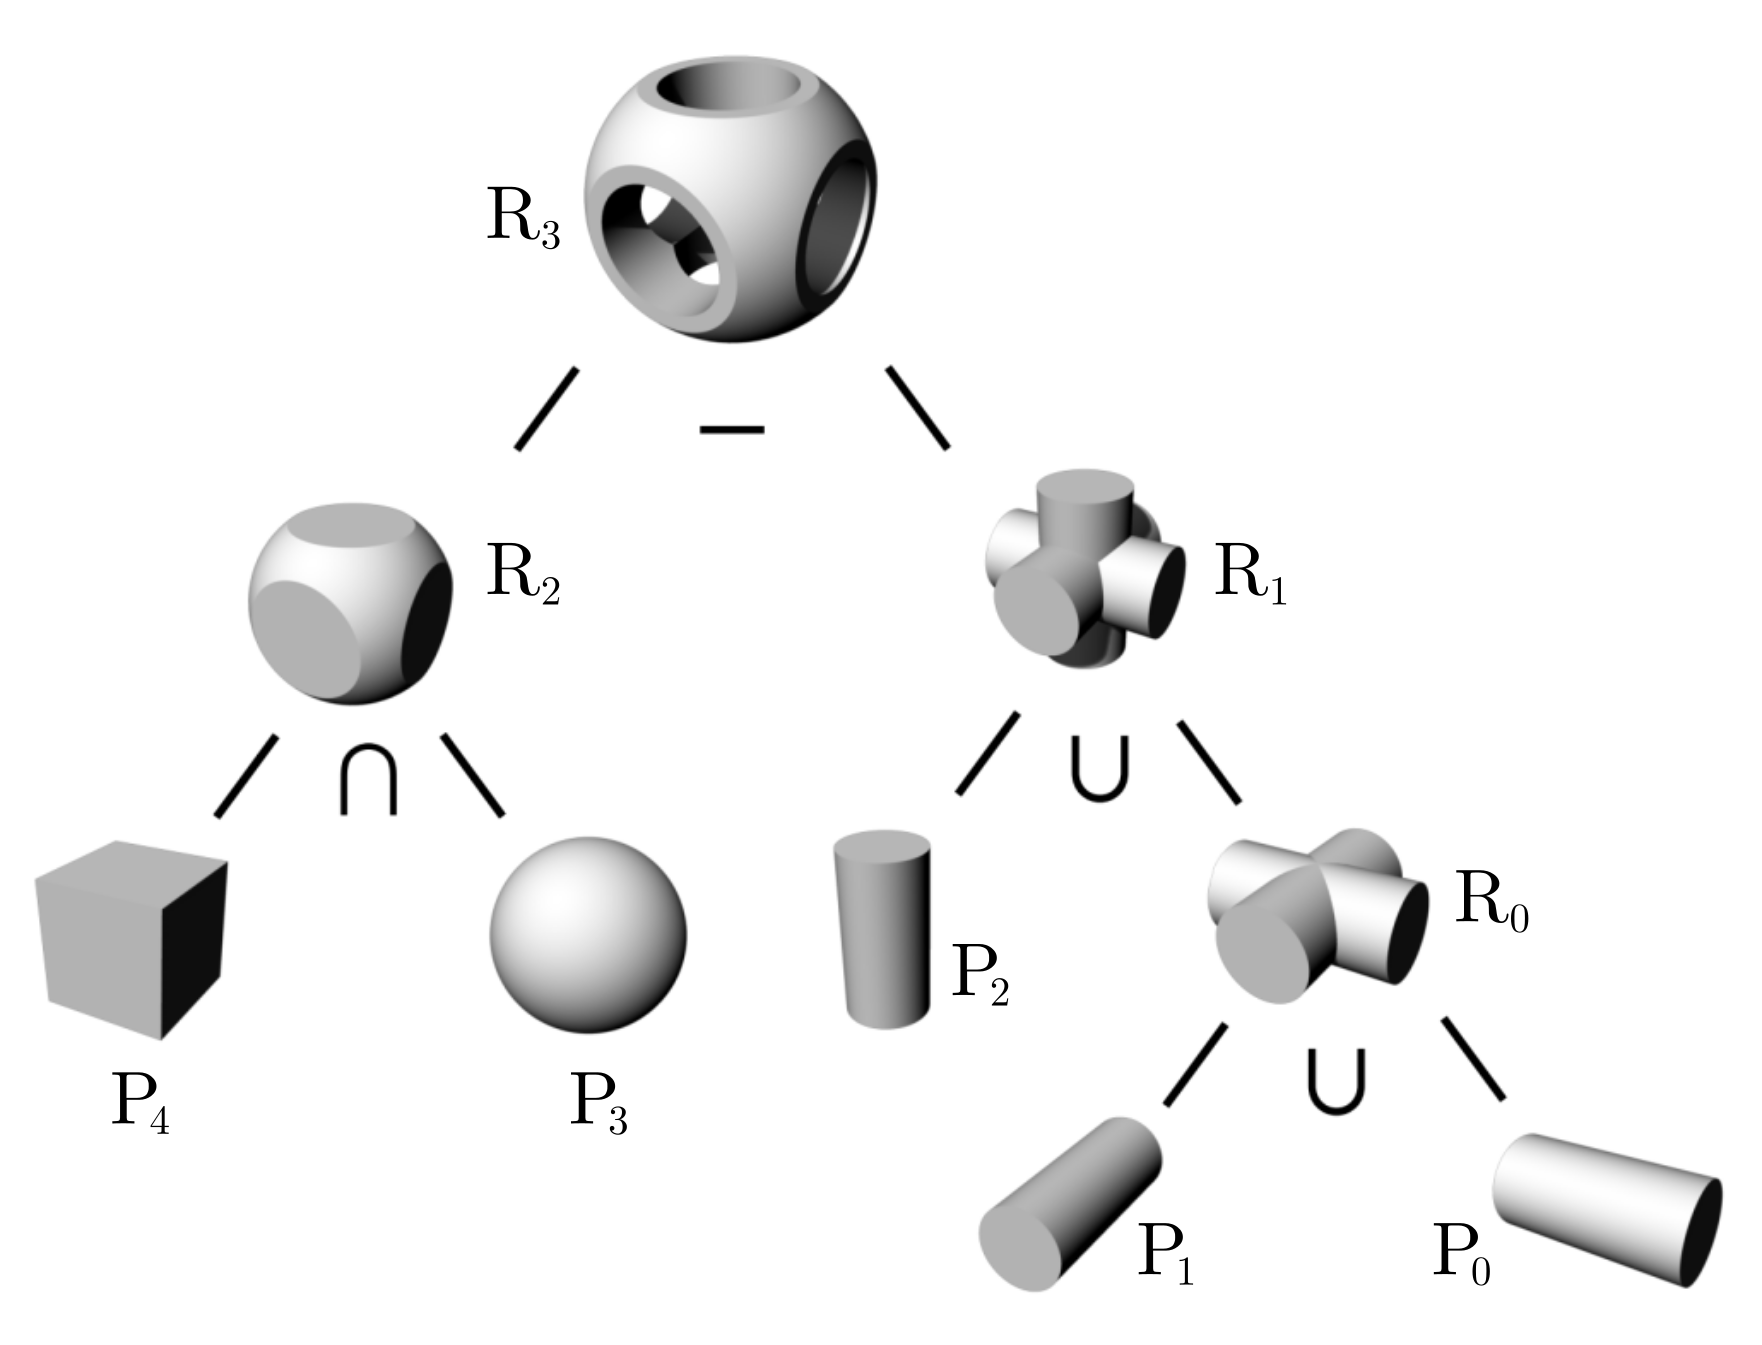
\includegraphics[width=12cm]{Img/GEO/geo-booleano6.png}
\centering
\caption{\textbf{Figura 3.11. \footnotesize{Arbol CSG con tres operaciones booleanas: unión $\cup$, intersección $\cap$ y diferencia $-$. }}}
\end{figure}

En el ejemplo de la figura 13 se puede ver la descripción de un modelo booleano, llamado R3.\vskip Partiendo de las primitivas $P_0$ (cilindro), $P_1$ (cilindro), $P_2$ (cilindro), $P_3$ (esfera) y $P_4$ (cubo) se obtiene el objeto final ($R_3$) después de tres niveles de operaciones booleanas.\vskip
En primer lugar se efectúa la unión de $P_0$ y $P_1$, después de haber transformado y posicionado adecuadamente las primitivas en el espacio, mediante las matrices netas $T_0$ y $T_1$.

$$R_0 = P_0\cdot T_0 \cup P_1\cdot T_1$$
A continuación el resultado intermedio $R_0$ se suma con la primitiva $P_2$ (cilindro), después de haber sido escalada y posicionada por $T_2$.

$$R_1 = R_0 \cup P_2\cdot T_2$$

Para producir el resultado $R_2$ se realiza la intersección entre $P_3$ y $P_4$, después de haber transformado y posicionado adecuadamente las primitivas en el espacio, mediante las matrices netas $T_3$ y $T_4$

$$R_2 = P_3\cdot T_3 \cap P_4\cdot T_4$$

Finalmente, a $R_2$ se le resta $R_1$, obteniéndose así el objeto raíz del árbol $R_3$.


$$
R_3 = R_2 - R_1 = (P_3\cdot T_3 \cap P_4\cdot T_4) - ((P_0\cdot T_0 \cup P_1\cdot T_1) \cup (P_2\cdot T_2))
$$

Se puede apreciar que las transformaciones han incrementado el tamaño del sólido resultante $R_3$. \vskip
El modelado booleano es un proceso descriptivo, es decir, sólo se limita a especificar qué primitivas se utilizan y cómo se combinan. En otras palabras, en los modelos booleanos sólo se dispone de la información geométrica y topológica de las primitivas, pero no la de los objetos modelados. Por tal motivo, también se les denomina modelos descriptivos y/o no evaluados, ya que para conocer sus características geométricas y topológicas es preciso efectuar un proceso de evaluación, conocido como evaluador de fronteras, que se encarga de hallar las intersecciones entre las superficies de las primitivas, para luego poder buscar los vértices y aristas. Además, ha de analizar la conectividad de los elementos encontrados, para determinar la topología del modelo.




Por lo general, el escalado de las primitivas no es uniforme, es decir, los factores de escala $Sx$, $Sy$, y $Sz$ son diferentes. De este modo, una sola primitiva proporciona una infinita variedad de copias diferentes.\vskip
Para poder combinar las primitivas en un esquema de modelado, éstas han de ser definidas previamente. Una forma frecuente de crearlas es estableciendo los parámetros de las ecuaciones que las definen. Entre las primitivas más comunes se encuentran los cubos, esferas, cilindros, conos y toros. Los parámetros suelen ser longitudes, como radios, diámetros, alturas, etc.

\subsubsection { Definición de las primitivas }
Las primitivas son los únicos elementos de los modelos booleanos (sin evaluar) que disponen de la información geométrica y topológica. Por tal motivo, para su definición se ha de utilizar un método que permita el registro de dicha información.

\textbf{Definición algebraica de las primitivas}\vskip
A cada conjunto de puntos $\Re$ , en principio se le puede asignar una función característica $g_\Re(X): X$ \xrightarrow $\{0,1\}$, que indica si un punto cualquiera $X$ pertenece o no a $\Re$. En otras palabras, si

$$g_\Re(X) = 1 \Rightarrow X \in \Re$$
$$g_\Re(X) = 0 \Rightarrow X \notin \Re$$

Esta función característica no es de mucha ayuda cuando se trata de conjuntos de puntos generales (sillas, zapatos), ya que su definición sería bastante ardua. Sin embargo, existe una clase interesante de conjuntos de puntos, cuya función característica puede quedar representada por una ecuación algebraica sencilla, del tipo $F(x, y, z) = 0$, siendo $x, y, z$ variables reales. En estos conjuntos se cumple que:
$\forall X = (x, y, z)$, si $F(X) \geq 0 \Rightarrow X
\in \Re$ , si $F(X) < 0 \Rightarrow X \notin \Re$, es decir que pertenece al complementario de \Re.

\textbf{A) Semiespacios}

La función $F(X) = 0$ define una superficie que divide el espacio cartesiano en dos regiones o conjuntos de puntos. \textit{Estas dos regiones se llaman semiespacios y están representados por las funciones} $F(X)
\geq 0$ y $F(X) \leq 0$. Por lo tanto, la función $F(x, y, z)$ vale $0$ en la superficie, y toma valores distintos de $0$ en el interior del semiespacio que contiene los puntos que van a formar parte del sólido. Los semiespacios quedan representados matemáticamente mediante la función $F(x, y, z)$, y mediante la ecuación $f(x, y, z)
\geq 0$ o $f(x, y, z) \leq 0$. Ver
que en cualquier caso, los puntos de las superficies pertenecen a los semiespacios.\vskip
Como representante típico de los semiespacios tenemos el \textit{semiespacio planar}, cuya función característica es $A_x + B_y + C_z + D \geq 0$. Este semiespacio se define como la unión de los puntos del plano definido por $A_x + B_y + C_z + D = 0$ (conjunto de puntos de frontera $fR$), más los puntos de uno de los subespacios separados por el plano, en este caso el positivo (puntos de interior $iR$).\vskip
Otro ejemplo lo tenemos en el \textit{semiespacio cilíndrico}, formado por todos los puntos que se encuentran en el interior y en la superficie de un cilindro infinito, con el eje en Z. En este caso, su ecuación característica es $x^2 + y^2 - r^2 \leq 0$.\vskip
La figura 14 muestra los semiespacios anteriores. Las flechas señalan hacia los puntos que pertenecen al semiespacio.

\begin{figure}[h]
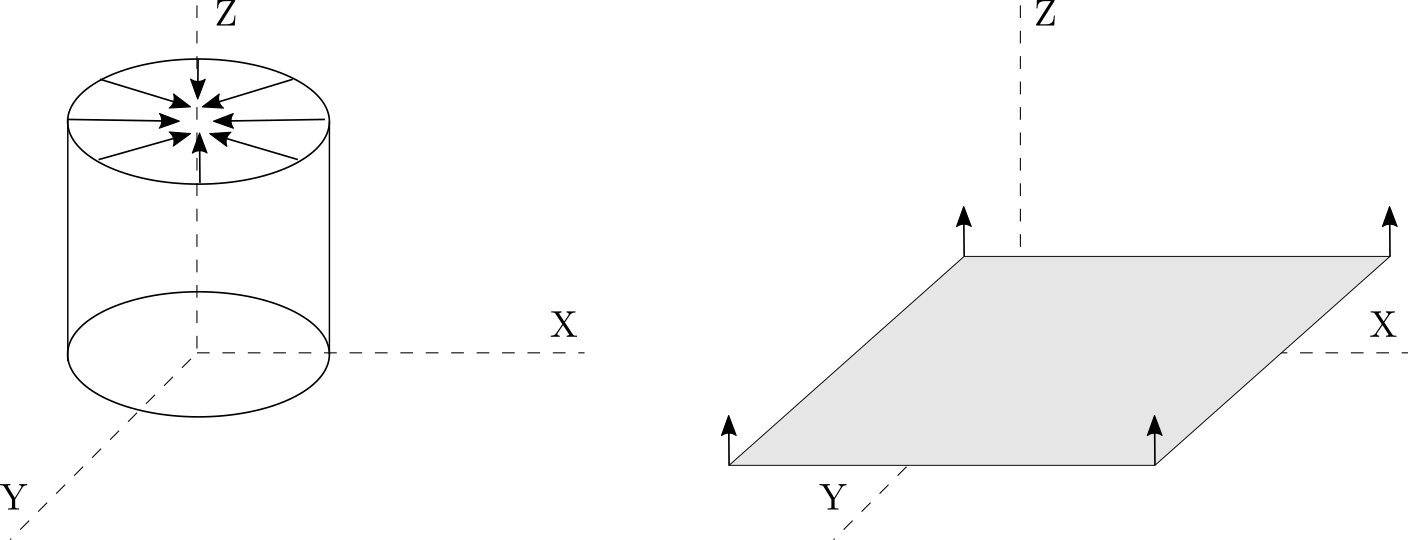
\includegraphics[width=12cm]{Img/GEO/geo-semiespacio0.png}
\centering
\caption{\textbf{Figura 3.11. \footnotesize{ejemplos de semiespacios abiertos. }}}
\end{figure}

Los ejemplos anteriores representan superficies ilimitadas que dividen el espacio cartesiano en dos regiones ilimitadas, generando semiespacios abiertos. Sin embargo, también puede haber semiespacios cerrados.\vskip
Así, la ecuación $x^2 + y^2 + z^2 – r^2 = 0$ define una superficie cerrada que divide el espacio cartesiano en una región ilimitada y otra limitada. La superficie representa una esfera de radio $r$, y el semiespacio esférico que genera queda definido por\vskip
$x^2 + y^2 + z^2 – r^2 \leq 0$, o sea, por todos los puntos que están dentro ($iR$) y en la superficie de la esfera ($fR$).
Otros semiespacios interesantes para modelado, definidos por ecuaciones características de grado 2 o superior, son los generados por las superficies cónicas (semiespacios cónicos abiertos, $x^2 + y^2 – z^2 \leq 0$), y por los toros (semiespacios tóricos cerrados, $(x^2 + y^2 + z^2 – (a^2 + b^2))^2 \leq 4a^2(b^2 – z^2)$.\vskip
La figura 15 muestra estos semiespacios, con los parámetros que intervienen en sus ecuaciones características.
\begin{figure}[h]
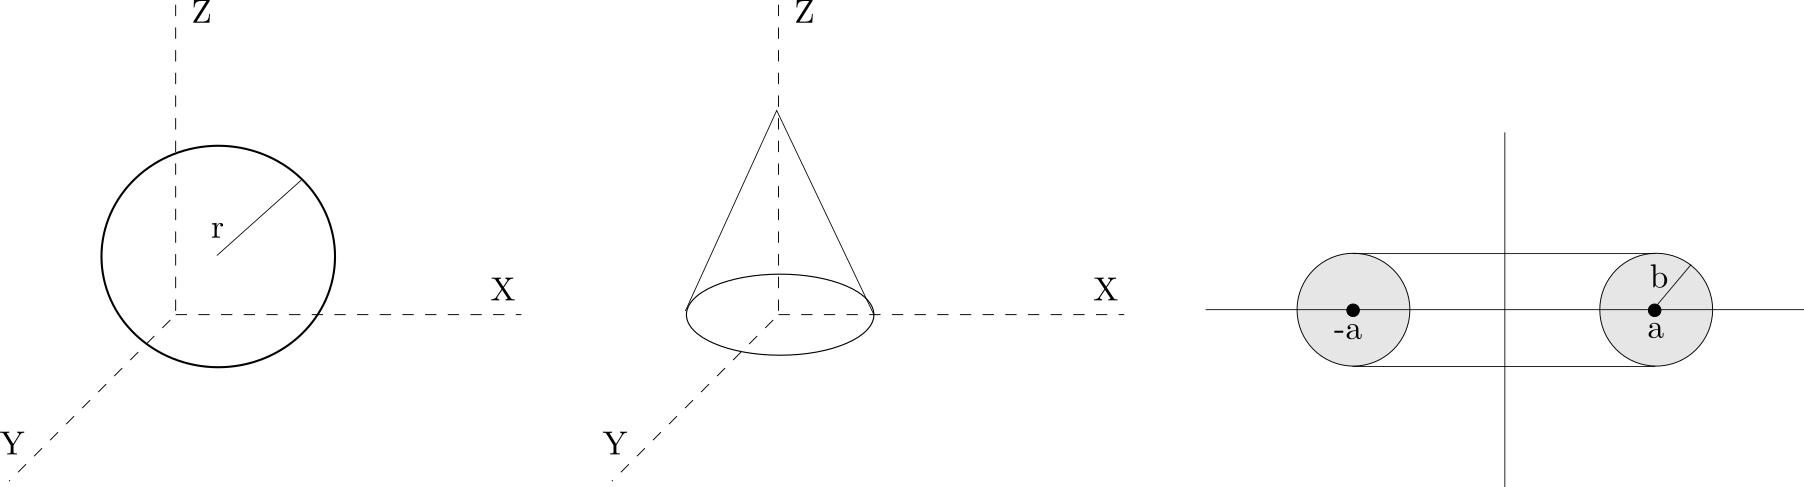
\includegraphics[width=16cm]{Img/GEO/geo-semiespacio1.png}
\centering
\caption{\textbf{Figura 3.11. \footnotesize{semiespacio esférico, cónico y tórico }}}
\end{figure}

En la figura 15 a la derecha se muestra una sección transversal del toro, que consiste en dos círculos, de radio $b$, centrados en $x = \pm a$, $z = 0$.

\textbf{B) Primitivas de espacios semiabiertos}\vskip
Por definición, el modelado booleano requiere que las primitivas sean sólidos cerrados. Por tanto, si un modelador desea utilizar semiespacios abiertos (planares, cilíndricos, cónicos, etc.) antes ha de efectuar una composición de semiespacios, de modo que el semiespacio resultante sea un espacio cerrado.\vskip
Como los semiespacios son conjuntos de puntos, los procesos naturales para crear primitivas cerradas a partir de semiespacios abiertos, no son otros que los operadores booleanos regularizados de unión, intersección y diferencia, aunque normalmente, con la intersección es suficiente. En definitiva, \textit{las primitivas que requieren semiespacios abiertos en su definición, se construyen combinando copias de semiespacios, mediante operaciones booleanas}.\vskip
En el ejemplo se utilizan semiespacios abiertos diferentes para crear una primitiva, lo encontramos en la figura 16.
En este caso, se trata de crear un cilindro cerrado. Para ello, se utiliza un semiespacio cilíndrico y dos planares, orientados según muestra la figura. Las ecuaciones características de estos semiespacios son:
\begin{figure}[h]
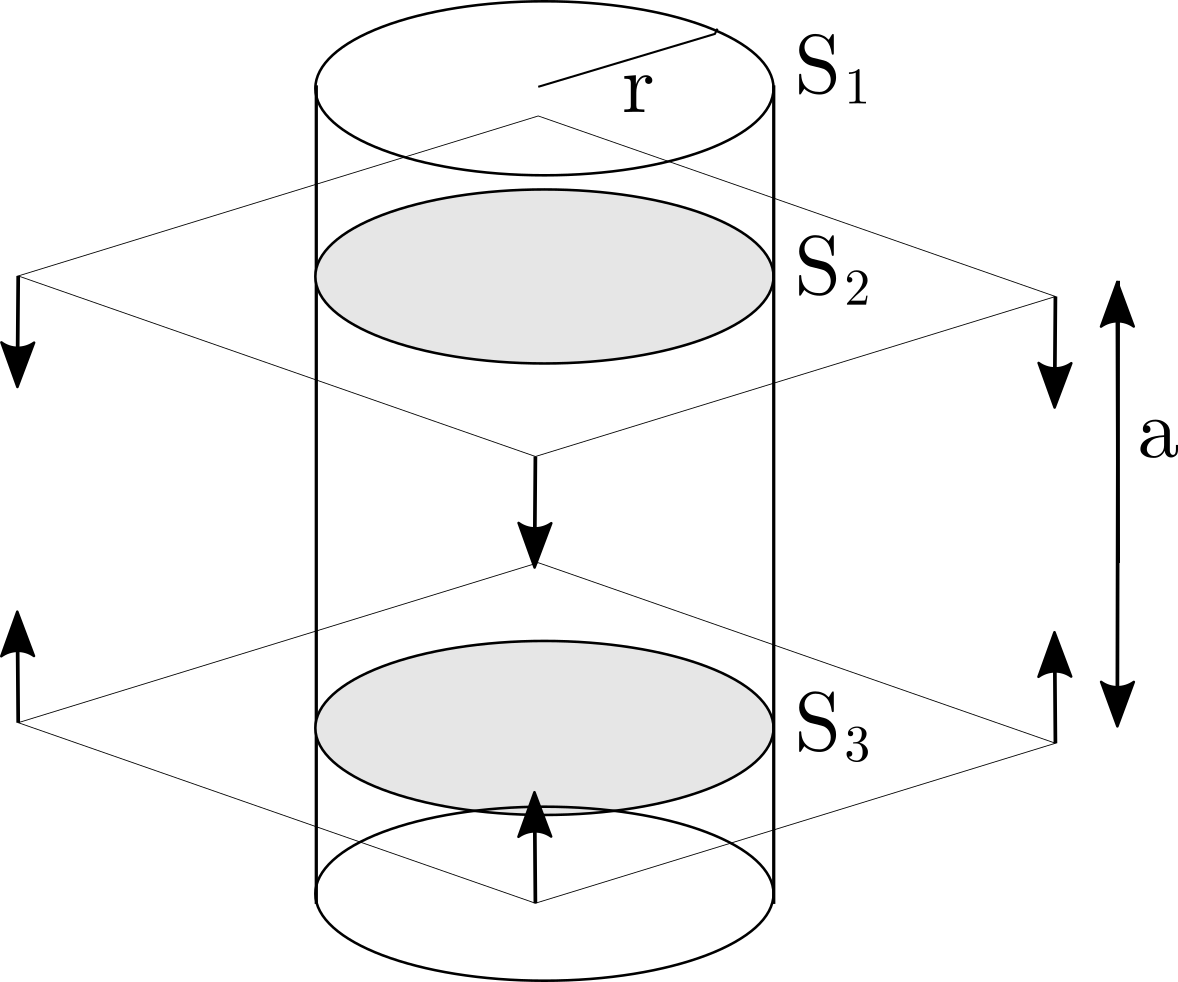
\includegraphics[width=8cm]{Img/GEO/geo-semiespacio2.png}
\centering
\caption{\textbf{Figura 3.11. \footnotesize{obtención de una primitiva (cilindro cerrado) a partir de semiespacios. }}}
\end{figure}

\begin{description}
\item $S_1$: $x^2 + z^2 − r^2 \leq 0$
\item $S_2$: $y\geq0$
\item $S3$: $y - a \leq 0$, siendo a la altura del cilindro.
\end{description}

El cilindro queda definido por: $C = S_1 \cap S_2 \cap S_3$


\subsubsection{Conjuntos de primitivas}
Una cuestión vital a la hora de crear un modelador booleano es la de \textit{establecer el conjunto de primitivas de que va a disponer el modelador}.\vskip
Se llama \textit{dominio o poder expresivo} de un modelador, a la \textit{capacidad que posee para modelar los diferentes objetos}. Cuanto mayor sea el poder expresivo de un modelador, mayores son las posibilidades de modelado.\vskip
El dominio de un sistema de modelado no depende del número de primitivas disponibles, sino que viene dado por \textit{la variedad de semiespacios utilizados al construir las primitivas, del conjunto de operadores booleanos desarrollados, y del total de operaciones de transformación disponibles}.

En principio, un sistema de modelado podría permitir al usuario aumentar el dominio y/o la potencia del modelador, dejándole definir sus propias primitivas. Esto implicaría que habría que comprobar, por parte del usuario mismo o del sistema, la validez de estas primitivas, creándose una incertidumbre sobre la integridad de los modelos. La mejor solución es que el sistema de modelado proporcione un conjunto completo de primitivas, de modo que no exista la necesidad de crear otras por parte del usuario. Éste, sólo se encargará de proporcionar los parámetros necesarios para manipular las primitivas, como p. e., la posición, orientación, forma y tamaño.


\subsection{ Constructive solid geometry (CSG) con algoritmos }
Agiliza el desarrollo y los detalles del diseño.
Mejora la visualización y la comunicación.
Elimina los problemas de interferencias del diseño.
Comprueba la funcionalidad y el rendimiento del diseño (sin la necesidad de prototipos físicos)
Proporciona de forma automática la fabricación con modelos sólidos en 3D, necesarios al programar máquinas herramienta de CNC y equipo de prototipos rápidos.

https://en.wikipedia.org/wiki/Constructive_solid_geometry

http://lsi.ugr.es/~cad/teoria/Tema5/RESUMENTEMA5.PDF

https://www.solidworks.es/sw/products/3d-cad/3d-solid-modeling.htm

http://cad3dconsolidworks.uji.es/CAD3DSW1_T1_Modelado_Cap01.pdf

\section{Modelos 3D en la web. 
}

http://evanw.github.io/csg.js/

\subsection{Representación de modelos sólidos en la web
}

\subsection{Data Exchange
}

\subsection{Sistemas de persistencia y parámetros
}

\subsection{Interfaces de manipulación directa}

\section{Trabajos relacionados y antecedentes}

\section{Problemas y recomendaciones
}